\documentclass[12pt]{article}
% load packages
\usepackage[german]{babel}
\usepackage[utf8]{inputenc}
\usepackage[a6paper,landscape]{geometry}
\usepackage{ifthen} % ifthenelse command
\usepackage{xifthen} % provides \isempty
\usepackage{amssymb}
\usepackage{xcolor}
\usepackage{graphicx} % for including pictures
\usepackage{xstring} %string operations
\usepackage{pgffor} %for-loop
\usepackage{amsmath} %for compoundfractions

\usepackage{units} % for nice units and unit-fractions

\usepackage{pifont} %define checkmark and xmark
\newcommand{\cmark}{\ding{51}}%
\newcommand{\xmark}{\ding{55}}%

\pagestyle{empty} % no page numbers
\setlength\parindent{0pt} %no indent

%%%%%%%%%%%%%%%%%%%%%%%%%%%%%%%%%%%%%%%%%%%%%%%%%%%%%%%%%%%%%%
%%%
%%% define search tags - edit to add more tags
%%%
% 4 Kategorien von Tags: 
% Kürzel, basales Jahr, Topic, und Schwierigkeitsgrad
%
% Um eine Kategorie zu erweitern, einfach unten in der Liste
% hinzufügen. Reihenfolge spielt keine Rolle.
% BEACHTE!! Nach dem letzten Eintrag in der Liste muss 
% ebenfalls ein Komma folgen.

% Liste: basale Phase
\newcommand{\basaltype}
{
basal1, %was sie beim Eintritt Gym1 wissen sollten
basal2, %was sie Ende Gym1 wissen sollten
}

% Liste: different topics
\newcommand{\topic}
{
LineareFunktionen, %balsal2
Bruchgleichungen,%balsal2
Pythagoras,%balsal1
Einheiten,%balsal1
Proportionalitäten,%balsal1
Kreisberechnung,%balsal1{}
Dreieck,%balsal1
Viereck,%balsal1
n-Ecke,%balsal1 (bis n=4)
Termumformungen,%balsal1 und basal2
Grundoperationen, %balsal1 und basal2
Kongruenz,%balsal1
Ähnlichkeit,%balsal2
Mathematisieren,%balsal1 und basal2
Funktionsauswertung,%balsal2
Koordinatensystem,%basal1 und basal2
Bruchrechnen,%balsal1
Wurzel,%balsal1
Begrifflichkeiten, %balsal1 und basal2 (Betrag)
BinomischeFormeln, %balsal2
Potenzen,%balsal2
}

% Liste: degree of diffculty
\newcommand{\difficulty}
{
leicht, 
mittel, 
schwer,
}
%%%%%%%%%%%%%%%%%%%%%%%%%%%%%%%%%%%%%%%%%%%%%%%%%%%%%%%%%%%%

%%%
%%% 'question' interface
%%%
\newcommand{\question}[1]{ 
\\ #1
}

%%%
%%% 'solution' interface
%%%
\newcommand{\solution}[1]{
%\vfill\hfill $\rightarrow$ Lösung: #1
\vfill\color{red} #1
}

%%%
%%% 'extract' command
%%%
\newcommand{\extract}[2]{
    \StrDel{#1}{,}[\mytempinput]% delete commas from string
    \StrLen{#1}[\len]% if empty string, add dummy character
    \ifthenelse{\equal{\len}{0}}{\let\mytempinput=a}{\ignorespaces}
    \foreach \tag in #2 {% loop through the list of expressions
        \IfSubStr{\mytempinput}{\tag}{%
            \StrDel{\mytempinput}{\tag}[\mytempinput]%
            \tag\ %if found in string, print expression
        }{%
            \ignorespaces % otherwise do nothing
        }%
        \global\let\mytempinput=\mytempinput% export outside
    }%
    %
    \StrLen{\mytempinput}[\len]%
    \ifthenelse{\equal{\len}{0}}{\ignorespaces}{\xmark}%
}

%%%
%%% 'add' interface 
%%%
\newenvironment{Add}[4]
{
    \hspace*{\fill} 
    {\it \tiny Tags found:
    % extract Kürzel - make cross if empty 
    \ifthenelse {\isempty{#1}} {\xmark}{#1} $|$%
    % extract basal type - make cross if empty of strange string
    \extract{#2}{\basaltype} $|$%
    % extract topics - make cross if empty of strange string
    \extract{#3}{\topic} $|$%
    % extract degree of difficulty - make cross if empty of strange string
    \extract{#4}{\difficulty}%
    }
    \\
    \noindent\rule{\textwidth}{1pt}% horizontal line
}
    %add question and solution
{
    \newpage
}

\usepackage{pagecolor}
\begin{document}
\pagecolor{lightgray!30}

\begin{Add}{BiT}{basal1}{Grundoperationen}{leicht}
\question{ Vereinfache $a+a+a$ }
\solution{ }
\end{Add}
\begin{Add}{BiT}{basal1}{Grundoperationen}{leicht}
\question{ Vereinfache $a+a+a$ }
\solution{ $3a$ }
\end{Add}

\begin{Add}{HaeK}{basal1}{BinomischeFormeln}{leicht}
\question{ Ergänze den Ausdruck: $(2x+3)^2=4x^2+....+9$ }
\solution{ }
\end{Add}
\begin{Add}{HaeK}{basal1}{BinomischeFormeln}{leicht}
\question{ Ergänze den Ausdruck: $(2x+3)^2=4x^2+....+9$ }
\solution{ $4x^2+12x+9$ }
\end{Add}

\begin{Add}{HaeK}{basal1}{Einheiten}{leicht}
\question{ Übersetze 1 Liter in die Einheit dm$^3$. }
\solution{ }
\end{Add}
\begin{Add}{HaeK}{basal1}{Einheiten}{leicht}
\question{ Übersetze 1 Liter in die Einheit dm$^3$. }
\solution{ 1\,dm$^3$ }
\end{Add}

\begin{Add}{HaeK}{basal1}{n-Ecke,Begrifflichkeiten,Dreieck}{leicht}
\question{ Gib die Innenwinkelsumme eines Dreiecks an. }
\solution{ }
\end{Add}
\begin{Add}{HaeK}{basal1}{n-Ecke,Begrifflichkeiten,Dreieck}{leicht}
\question{ Gib die Innenwinkelsumme eines Dreiecks an. }
\solution{ $180^\circ$ }
\end{Add}

\begin{Add}{HaeK}{basal2}{Koordinatensystem,Begrifflichkeiten}{leicht}
\question{ In welchem Quadranten liegt der Punkt $(-1;5)$? }
\solution{ }
\end{Add}
\begin{Add}{HaeK}{basal2}{Koordinatensystem,Begrifflichkeiten}{leicht}
\question{ In welchem Quadranten liegt der Punkt $(-1;5)$? }
\solution{ Im 2. Quadranten. }
\end{Add}

\begin{Add}{HaeK}{basal2}{Bruchrechnen}{mittel}
\question{ Vereinfache $\frac{125}{81}\cdot\frac{27}{25}$. }
\solution{ }
\end{Add}
\begin{Add}{HaeK}{basal2}{Bruchrechnen}{mittel}
\question{ Vereinfache $\frac{125}{81}\cdot\frac{27}{25}$. }
\solution{ $\frac{5}{3}$ }
\end{Add}

\begin{Add}{HaeK}{basal2}{Potenzen,Grundoperationen}{leicht}
\question{ Berechne $-2^2$. }
\solution{ }
\end{Add}
\begin{Add}{HaeK}{basal2}{Potenzen,Grundoperationen}{leicht}
\question{ Berechne $-2^2$. }
\solution{ $-4$ }
\end{Add}

\begin{Add}{HaeK}{basal2}{Potenzen}{leicht}
\question{ Berechne $7.2\cdot10^7 -1.8\cdot10^{6}$. }
\solution{ }
\end{Add}
\begin{Add}{HaeK}{basal2}{Potenzen}{leicht}
\question{ Berechne $7.2\cdot10^7 -1.8\cdot10^{6}$. }
\solution{ $7.02\cdot10^7$ }
\end{Add}

\begin{Add}{HaeK}{basal2}{BinomischeFormeln,Termumformungen}{mittel}
\question{ Multipliziere $(2x+\sqrt{x+5})^2$ aus. }
\solution{ }
\end{Add}
\begin{Add}{HaeK}{basal2}{BinomischeFormeln,Termumformungen}{mittel}
\question{ Multipliziere $(2x+\sqrt{x+5})^2$ aus. }
\solution{ $4x^2+4x\sqrt{x+5}+x+5$ }
\end{Add}

\begin{Add}{HaeK}{basal2}{Mathematisieren}{leicht}
\question{ Übersetze in eine Gleichung: a ist um 4 grösser als b. }
\solution{ }
\end{Add}
\begin{Add}{HaeK}{basal2}{Mathematisieren}{leicht}
\question{ Übersetze in eine Gleichung: a ist um 4 grösser als b. }
\solution{ $a=b+4$ }
\end{Add}

\begin{Add}{HaeK}{basal2}{Mathematisieren}{leicht}
\question{ Übersetze in eine Gleichung: a ist um 4 kleiner als b. }
\solution{ }
\end{Add}
\begin{Add}{HaeK}{basal2}{Mathematisieren}{leicht}
\question{ Übersetze in eine Gleichung: a ist um 4 kleiner als b. }
\solution{ $a=b-4$ }
\end{Add}

\begin{Add}{HaeK}{basal2}{Grundoperationen}{leicht}
\question{ Teile die Gleichung $4x+7=8y-1$ durch 4. }
\solution{ }
\end{Add}
\begin{Add}{HaeK}{basal2}{Grundoperationen}{leicht}
\question{ Teile die Gleichung $4x+7=8y-1$ durch 4. }
\solution{ $x+\frac{7}{4}=2y-0.25$ }
\end{Add}

\begin{Add}{HaeK}{basal2}{Potenzen}{leicht}
\question{ Berechne $(-1)^{456987}$. }
\solution{ }
\end{Add}
\begin{Add}{HaeK}{basal2}{Potenzen}{leicht}
\question{ Berechne $(-1)^{456987}$. }
\solution{ $-1$ }
\end{Add}

\begin{Add}{HaeK}{basal2}{Potenzen}{leicht}
\question{ Berechne $(-1)^{456978}$. }
\solution{ }
\end{Add}
\begin{Add}{HaeK}{basal2}{Potenzen}{leicht}
\question{ Berechne $(-1)^{456978}$. }
\solution{ $1$ }
\end{Add}

\begin{Add}{HaeK}{basal2}{Potenzen}{mittel}
\question{ Ordne $2^{-3}, 2^3,(-2)^{-3}, (-2)^3$ nach aufsteigender Grösse. }
\solution{ }
\end{Add}
\begin{Add}{HaeK}{basal2}{Potenzen}{mittel}
\question{ Ordne $2^{-3}, 2^3,(-2)^{-3}, (-2)^3$ nach aufsteigender Grösse. }
\solution{ $(-2)^3=-8, (-2)^{-3}=-\frac{1}{8}, 2^{-3}=\frac{1}{8}, 2^3=8$ }
\end{Add}

            \begin{Add}{HaeK}{basal1}{Bruchrechnen}{schwer}
            \question{ Welcher Bruch hat einen anderen Wert als die drei anderen?

$$\dfrac{4}{-3}, \dfrac{-4}{-3}, -\dfrac{4}{3}, \dfrac{-4}{3}$$ }
            \solution{ }
            \end{Add}
            \begin{Add}{HaeK}{basal1}{Bruchrechnen}{schwer}
            \question{ Welcher Bruch hat einen anderen Wert als die drei anderen?

$$\dfrac{4}{-3}, \dfrac{-4}{-3}, -\dfrac{4}{3}, \dfrac{-4}{3}$$ }
            \solution{ $\frac{-4}{-3}=\frac{4}{3}$ }
            \end{Add}
            

    \begin{Add}{HaeK}{basal1}{Kreisberechnung}{mittel}
    \question{ Gib den Umfang des Kreissektors an.
\begin{center}
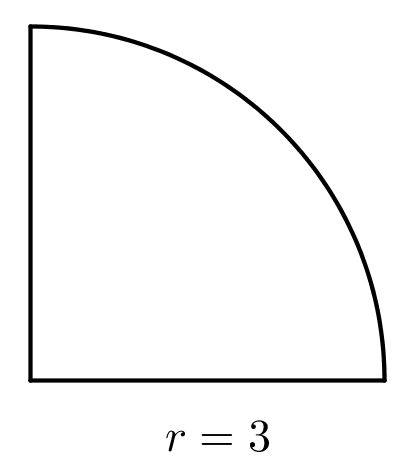
\includegraphics[width=0.3\textwidth]{pics/ViertelKreis}
\end{center} }
    \solution{ }
    \end{Add}
    \begin{Add}{HaeK}{basal1}{Kreisberechnung}{mittel}
    \question{ Gib den Umfang des Kreissektors an.
\begin{center}
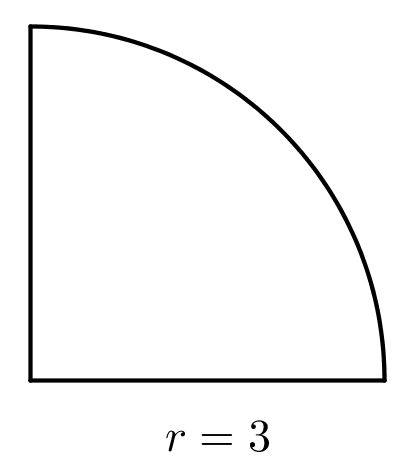
\includegraphics[width=0.3\textwidth]{pics/ViertelKreis}
\end{center} }
    \solution{ $6+\frac{3}{2}\pi$ }
    \end{Add}
    

     \begin{Add}{HaeK}{basal2}{Proportionalitäten}{mittel}
     \question{ Gib die Funktionsgleichung des Graphen an.
\vspace{-0.2cm}
 \begin{center}
 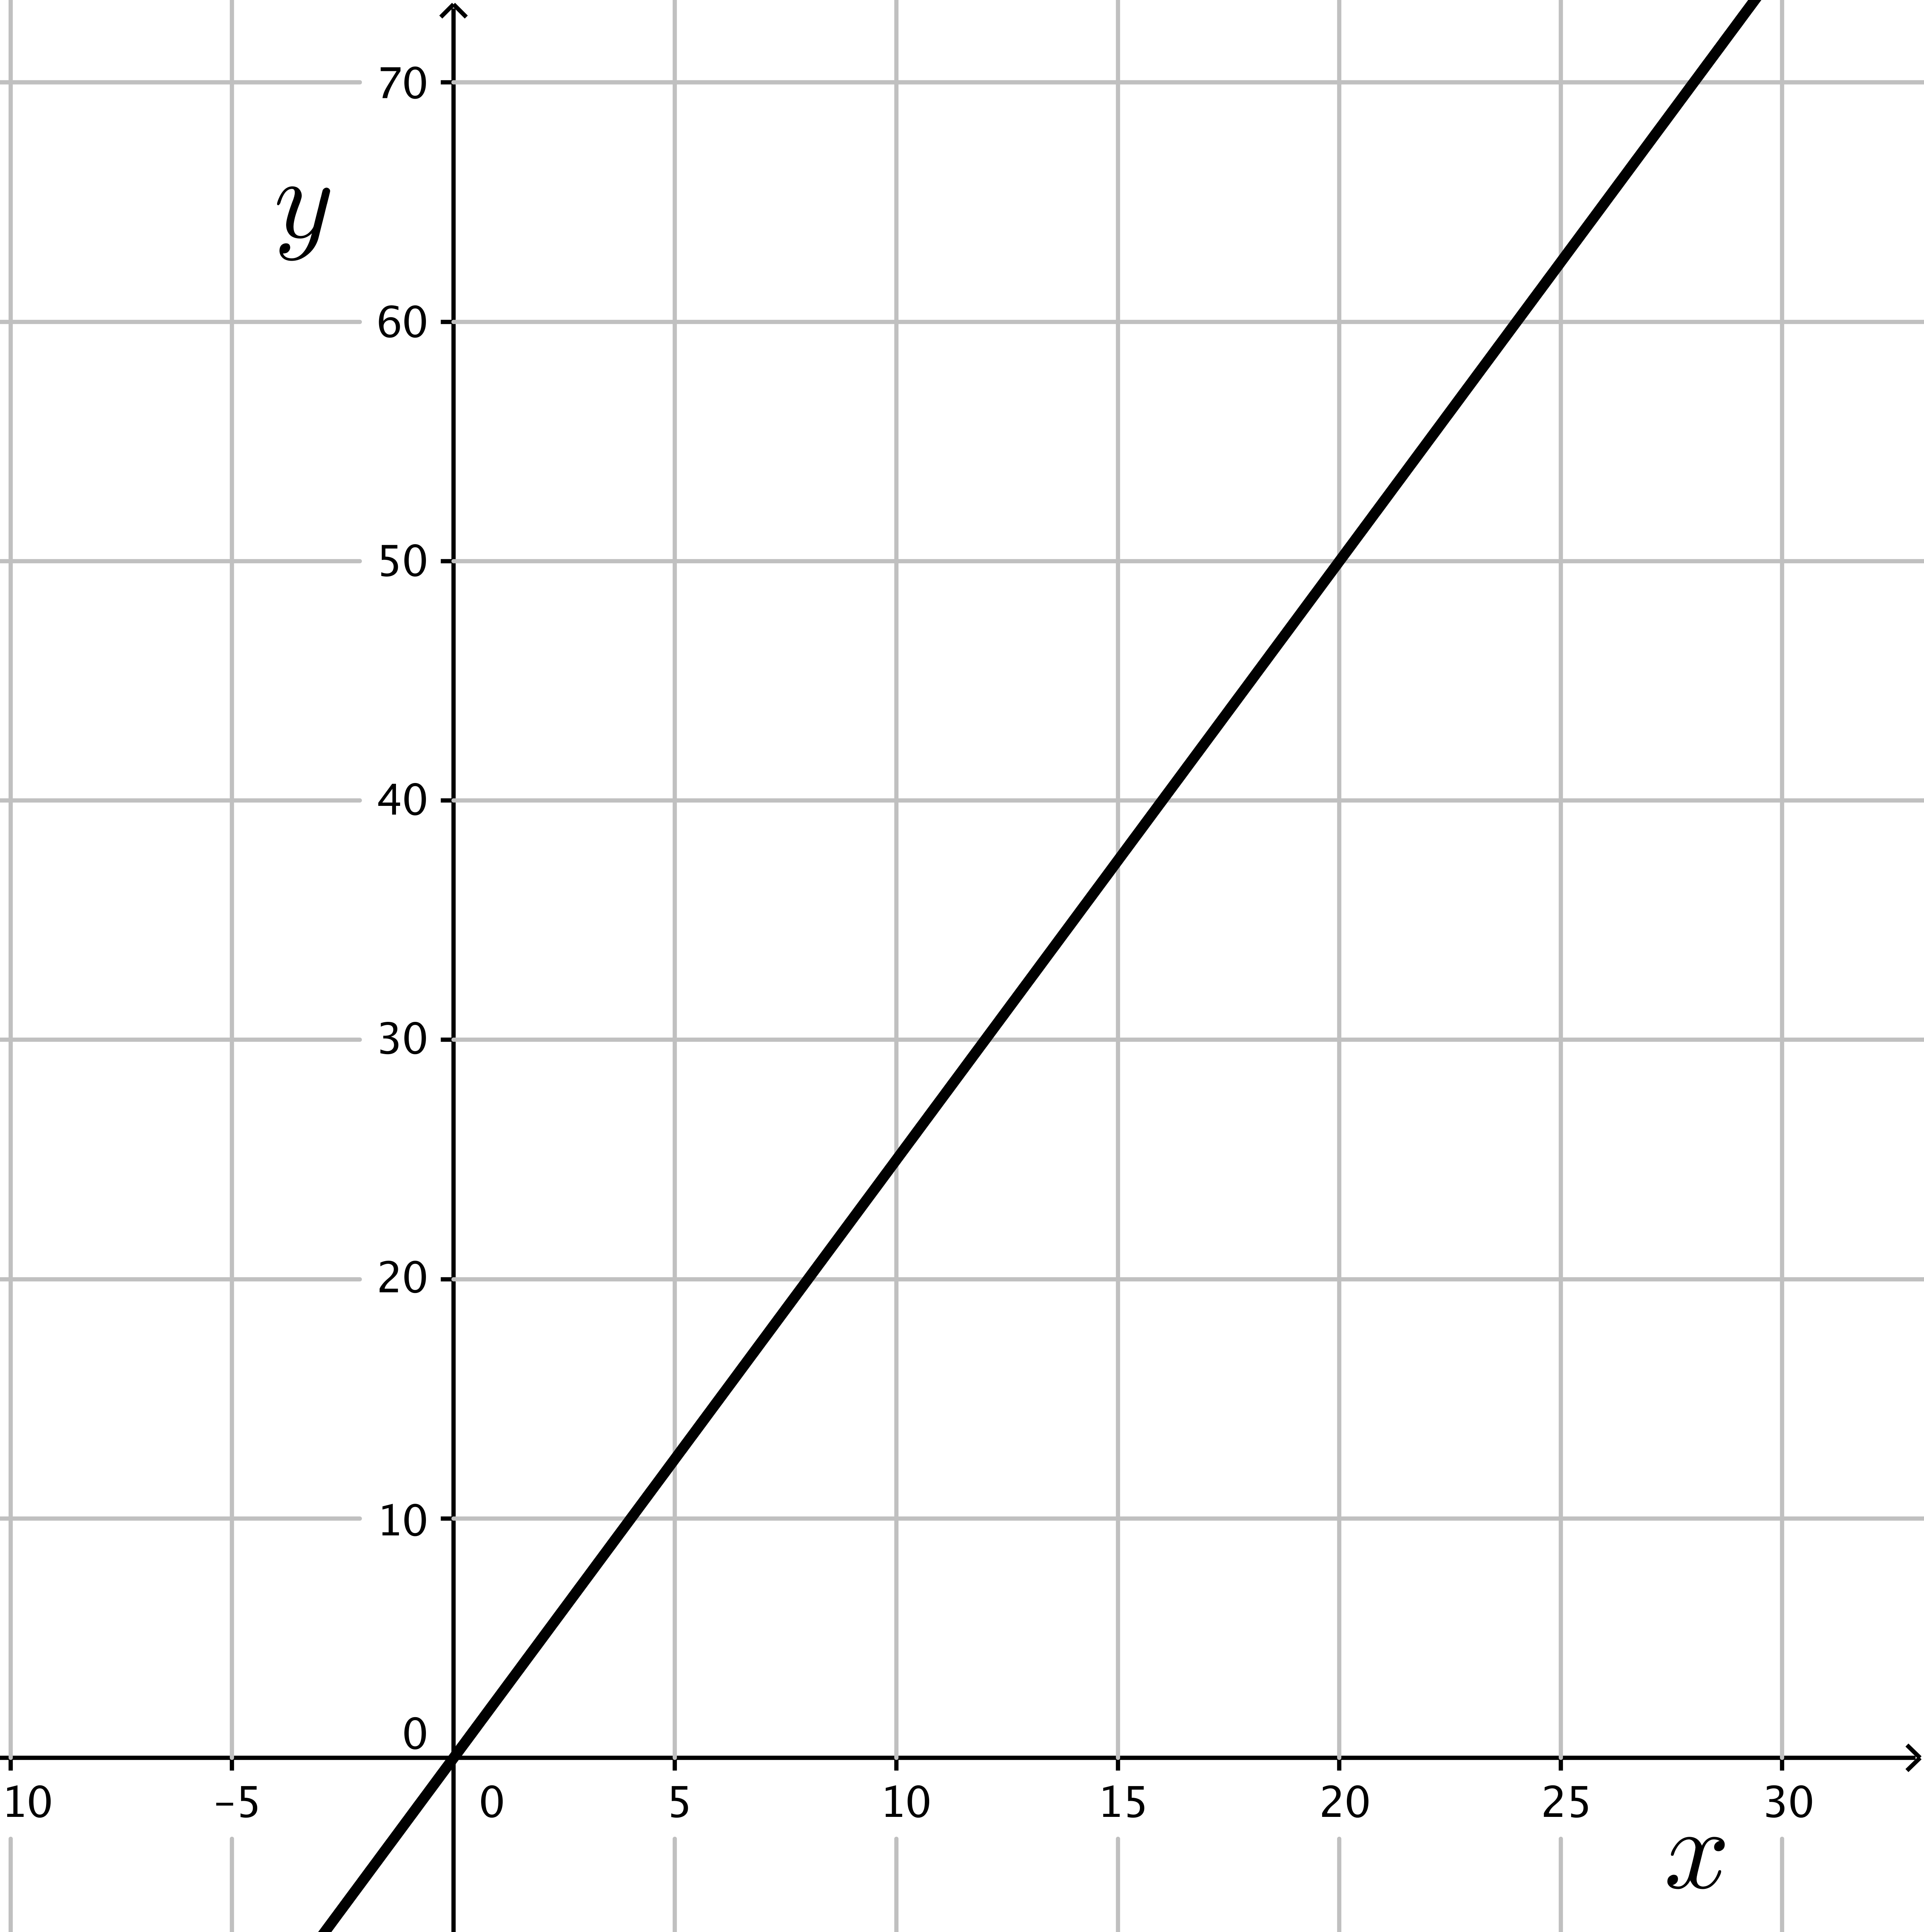
\includegraphics[width=0.45\textwidth]{pics/PropAchseSkal}
 \end{center}
 \vspace{-0.2cm} }
     \solution{ }
     \end{Add}
     \begin{Add}{HaeK}{basal2}{Proportionalitäten}{mittel}
     \question{ Gib die Funktionsgleichung des Graphen an.
\vspace{-0.2cm}
 \begin{center}
 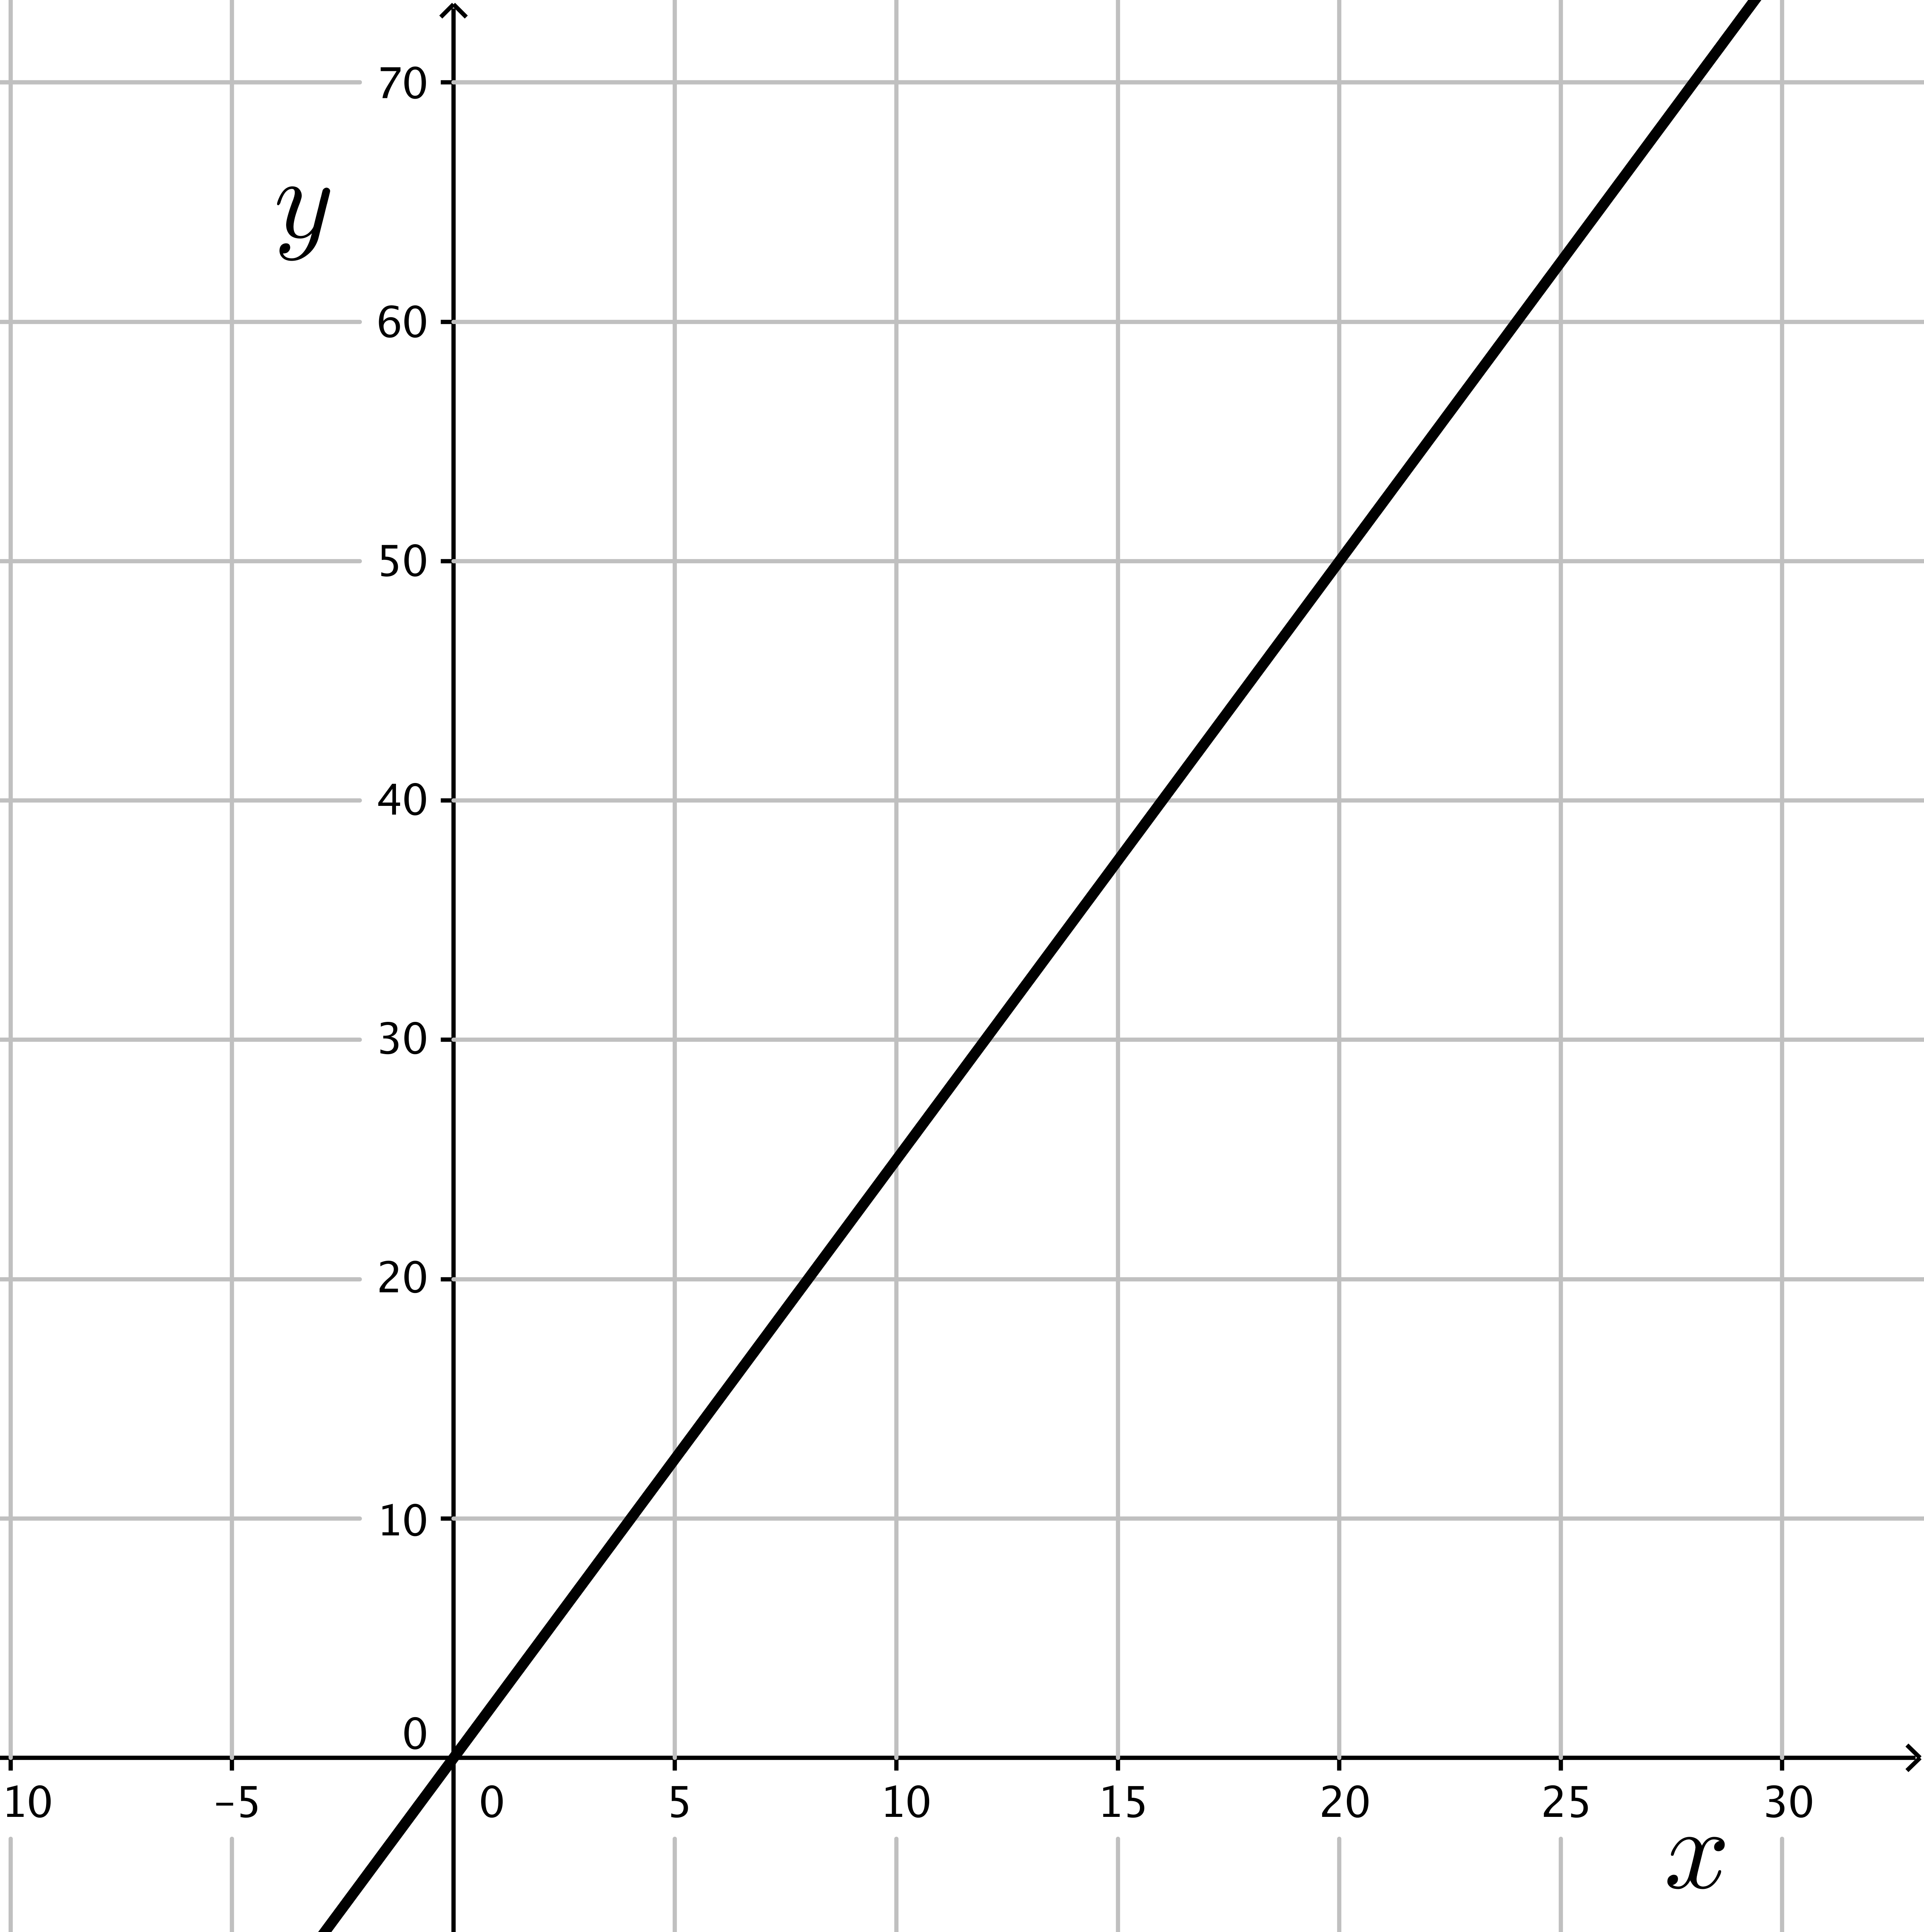
\includegraphics[width=0.45\textwidth]{pics/PropAchseSkal}
 \end{center}
 \vspace{-0.2cm} }
     \solution{ $y=2.5x$ }
     \end{Add}
     

\begin{Add}{HaeK}{basal2}{Funktionsauswertung}{mittel}
\question{ Drücke die Aussage \glqq Durch die Funktion $f$ wird der Zahl 2 die Zahl 78 zugeordnet\grqq\ in mathematischer Schreibweise aus. }
\solution{ }
\end{Add}
\begin{Add}{HaeK}{basal2}{Funktionsauswertung}{mittel}
\question{ Drücke die Aussage \glqq Durch die Funktion $f$ wird der Zahl 2 die Zahl 78 zugeordnet\grqq\ in mathematischer Schreibweise aus. }
\solution{ $f(2)=78$ }
\end{Add}

\begin{Add}{BiT}{basal2}{Grundoperationen}{leicht}
\question{ Vereinfache $a\cdot a \cdot a$ }
\solution{ }
\end{Add}
\begin{Add}{BiT}{basal2}{Grundoperationen}{leicht}
\question{ Vereinfache $a\cdot a \cdot a$ }
\solution{ $a^3$ }
\end{Add}

    \begin{Add}{WiD}{basal1}{Pythagoras}{leicht}
    \question{ Berechne in einem rechtwinkligen Dreieck die Kathete $a$ falls $b=4$ und $c=5$.
\begin{center}
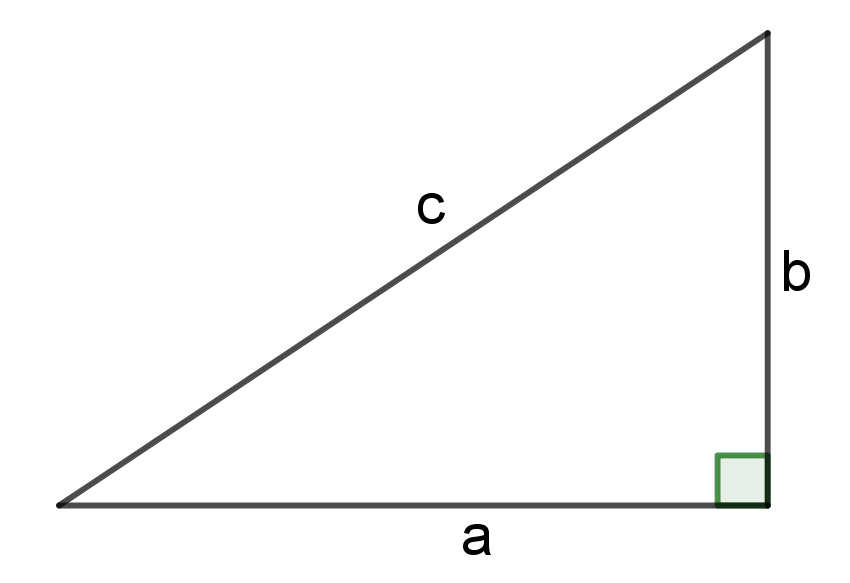
\includegraphics[width=0.5\textwidth]{pics/triangle}
\end{center} }
    \solution{ }
    \end{Add}
    \begin{Add}{WiD}{basal1}{Pythagoras}{leicht}
    \question{ Berechne in einem rechtwinkligen Dreieck die Kathete $a$ falls $b=4$ und $c=5$.
\begin{center}
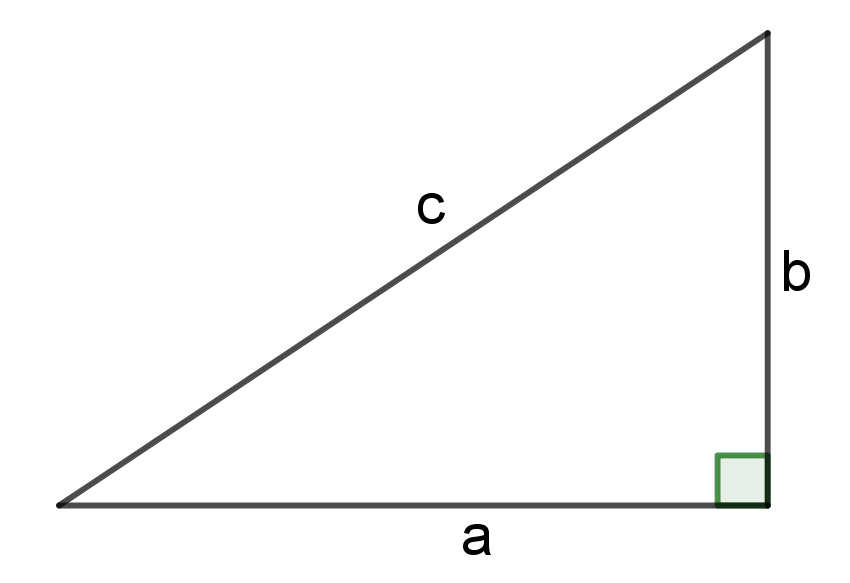
\includegraphics[width=0.5\textwidth]{pics/triangle}
\end{center} }
    \solution{ $c^2=a^2+b^2 \rightarrow a=3$ }
    \end{Add}
    

\begin{Add}{WiD}{basal1}{Ähnlichkeit}{leicht}
\question{ In einem gleichschenkligen Dreieck misst der eine Basiswinkel $\alpha=37^{\circ}$. Berechne die restlichen Winkel im Dreieck. }
\solution{ }
\end{Add}
\begin{Add}{WiD}{basal1}{Ähnlichkeit}{leicht}
\question{ In einem gleichschenkligen Dreieck misst der eine Basiswinkel $\alpha=37^{\circ}$. Berechne die restlichen Winkel im Dreieck. }
\solution{ $\alpha=\beta=37^{\circ} \rightarrow \gamma=180^{\circ}-2\cdot 37^{\circ}=106^{\circ}$ }
\end{Add}

    \begin{Add}{WiD}{basal1}{Dreieck}{leicht}
    \question{ Was ist korrekt? \\
Der Inkreismittelpunkt eines Dreiecks ist der Schnittpunkt der
\begin{itemize}
    \item[a)] Seitenhalbierenden
    \item[b)] Mittelsenkrechten
    \item[c)] Winkelhalbierenden
    \item[d)] Höhenlinien
\end{itemize} }
    \solution{ }
    \end{Add}
    \begin{Add}{WiD}{basal1}{Dreieck}{leicht}
    \question{ Was ist korrekt? \\
Der Inkreismittelpunkt eines Dreiecks ist der Schnittpunkt der
\begin{itemize}
    \item[a)] Seitenhalbierenden
    \item[b)] Mittelsenkrechten
    \item[c)] Winkelhalbierenden
    \item[d)] Höhenlinien
\end{itemize} }
    \solution{ c) }
    \end{Add}
    

\begin{Add}{WiD}{basal1}{Dreieck}{leicht}
\question{ In welchem Dreieck entspricht eine Scwerelinie gerade einer Winkelhalbierenden? }
\solution{ }
\end{Add}
\begin{Add}{WiD}{basal1}{Dreieck}{leicht}
\question{ In welchem Dreieck entspricht eine Scwerelinie gerade einer Winkelhalbierenden? }
\solution{ In einem gleichschenkligen }
\end{Add}

\begin{Add}{WiD}{basal1}{Dreieck}{leicht}
\question{ In welchem Dreieck liegt der Umkreismittelpunkt auf einer Seite? }
\solution{ }
\end{Add}
\begin{Add}{WiD}{basal1}{Dreieck}{leicht}
\question{ In welchem Dreieck liegt der Umkreismittelpunkt auf einer Seite? }
\solution{ In einem rechtwinkligen }
\end{Add}

    \begin{Add}{WiD}{basal1}{Viereck}{leicht}
    \question{ Welche Aussagen über Rhomben sind korrekt? \\
\begin{itemize}
    \item[a)] Im Rhombus halbieren sich die Diagonalen.
    \item[b)] Zwei gegenüberliegende Winkel ergänzen sich zu $180^{\circ}$.
    \item[c)] Ein Rhombus ist ein Rechteck.
    \item[d)] Gegenüberliegende Seiten sind parallel.
\end{itemize} }
    \solution{ }
    \end{Add}
    \begin{Add}{WiD}{basal1}{Viereck}{leicht}
    \question{ Welche Aussagen über Rhomben sind korrekt? \\
\begin{itemize}
    \item[a)] Im Rhombus halbieren sich die Diagonalen.
    \item[b)] Zwei gegenüberliegende Winkel ergänzen sich zu $180^{\circ}$.
    \item[c)] Ein Rhombus ist ein Rechteck.
    \item[d)] Gegenüberliegende Seiten sind parallel.
\end{itemize} }
    \solution{ a),d) }
    \end{Add}
    

    \begin{Add}{WiD}{basal1}{Bruchrechnen}{mittel}
    \question{ Vereinfache soweit als möglich \\
$$\frac{1}{a-1}-\frac{a+1}{a^2-1}+\frac{1}{a}$$ }
    \solution{ }
    \end{Add}
    \begin{Add}{WiD}{basal1}{Bruchrechnen}{mittel}
    \question{ Vereinfache soweit als möglich \\
$$\frac{1}{a-1}-\frac{a+1}{a^2-1}+\frac{1}{a}$$ }
    \solution{ $\frac{1}{a}$ }
    \end{Add}
    

    \begin{Add}{WiD}{basal1}{Koordinatensystem}{leicht}
    \question{ Spiegle den Punkt $A=(2;5)$ an der \begin{itemize}
    \item[a)] $x$-Achse 
    \item[b)] $y$- Achse
\end{itemize} }
    \solution{ }
    \end{Add}
    \begin{Add}{WiD}{basal1}{Koordinatensystem}{leicht}
    \question{ Spiegle den Punkt $A=(2;5)$ an der \begin{itemize}
    \item[a)] $x$-Achse 
    \item[b)] $y$- Achse
\end{itemize} }
    \solution{ a) $A'=(2;-5)$ \quad b) $A''=(-2;5)$ }
    \end{Add}
    

\begin{Add}{WiD}{basal1}{Koordinatensystem}{mittel}
\question{ Spiegle den Punkt $A=(-2;5)$ am Punkt $S=(1;4)$ }
\solution{ }
\end{Add}
\begin{Add}{WiD}{basal1}{Koordinatensystem}{mittel}
\question{ Spiegle den Punkt $A=(-2;5)$ am Punkt $S=(1;4)$ }
\solution{ $A'=(4;3)$ }
\end{Add}

\begin{Add}{WiD}{basal1}{Dreieck}{schwer}
\question{ Spannen die vier Punkte $A=(-9;3)$, $B=(-5;-3)$, $C=(1;1)$ und $D=(-3;7)$ ein Quadrat auf? Warum? }
\solution{ }
\end{Add}
\begin{Add}{WiD}{basal1}{Dreieck}{schwer}
\question{ Spannen die vier Punkte $A=(-9;3)$, $B=(-5;-3)$, $C=(1;1)$ und $D=(-3;7)$ ein Quadrat auf? Warum? }
\solution{ Ja, denn sowohl die Seitenlängen ($\sqrt{52}$) als auch die Diagonalen ($\sqrt{104}$) sind gleich lang }
\end{Add}

    \begin{Add}{WiD}{basal1}{Bruchrechnen}{mittel}
    \question{ Welcher Bruch ist kleiner? (Ohne 
Taschenrechner!)
\[ \dfrac{13}{17} \quad \text{ oder } \quad \dfrac{3}{4} \] }
    \solution{ }
    \end{Add}
    \begin{Add}{WiD}{basal1}{Bruchrechnen}{mittel}
    \question{ Welcher Bruch ist kleiner? (Ohne 
Taschenrechner!)
\[ \dfrac{13}{17} \quad \text{ oder } \quad \dfrac{3}{4} \] }
    \solution{ $\frac{3}{4}$ }
    \end{Add}
    

    \begin{Add}{WiD}{basal1}{Termumformungen}{leicht}
    \question{ Vereinfache soweit als möglich:
\[ 3x-6y-2(1+4x-3y) \] }
    \solution{ }
    \end{Add}
    \begin{Add}{WiD}{basal1}{Termumformungen}{leicht}
    \question{ Vereinfache soweit als möglich:
\[ 3x-6y-2(1+4x-3y) \] }
    \solution{ $-2-5x$ }
    \end{Add}
    

    \begin{Add}{WiD}{basal1}{Termumformungen}{leicht}
    \question{ Vereinfache soweit als möglich:
\[ 15a-\left((3a-6b)-c\right)-\left((5b-(-10a+4c)\right) \] }
    \solution{ }
    \end{Add}
    \begin{Add}{WiD}{basal1}{Termumformungen}{leicht}
    \question{ Vereinfache soweit als möglich:
\[ 15a-\left((3a-6b)-c\right)-\left((5b-(-10a+4c)\right) \] }
    \solution{ $2a+b-3c$ }
    \end{Add}
    

    \begin{Add}{WiD}{basal1}{Termumformungen}{leicht}
    \question{ Vereinfache soweit als möglich:
\[ -3(-2u)^3(1.5u)^2(-u)^4 \] }
    \solution{ }
    \end{Add}
    \begin{Add}{WiD}{basal1}{Termumformungen}{leicht}
    \question{ Vereinfache soweit als möglich:
\[ -3(-2u)^3(1.5u)^2(-u)^4 \] }
    \solution{ $54u^9$ }
    \end{Add}
    

    \begin{Add}{WiD}{basal1}{Termumformungen}{leicht}
    \question{ Multipliziere aus:
\[ (a+b)(1+a-b) \] }
    \solution{ }
    \end{Add}
    \begin{Add}{WiD}{basal1}{Termumformungen}{leicht}
    \question{ Multipliziere aus:
\[ (a+b)(1+a-b) \] }
    \solution{ $a^2+a+b-b^2$ }
    \end{Add}
    

    \begin{Add}{WiD}{basal1}{Termumformungen}{leicht}
    \question{ Multipliziere aus:
\[ (a^2+1)(a^2-a-1) \] }
    \solution{ }
    \end{Add}
    \begin{Add}{WiD}{basal1}{Termumformungen}{leicht}
    \question{ Multipliziere aus:
\[ (a^2+1)(a^2-a-1) \] }
    \solution{ $a^4-a^3-a-1$ }
    \end{Add}
    

    \begin{Add}{WiD}{basal1}{Termumformungen}{leicht}
    \question{ Welcher Term muss im Kasten \framebox[10mm]{\rule{0mm}{3mm}} stehen, damit die Gleichung erfüllt ist?
\[ 3x+4y-\framebox[10mm]{\rule{0mm}{3mm}}=x-y \] }
    \solution{ }
    \end{Add}
    \begin{Add}{WiD}{basal1}{Termumformungen}{leicht}
    \question{ Welcher Term muss im Kasten \framebox[10mm]{\rule{0mm}{3mm}} stehen, damit die Gleichung erfüllt ist?
\[ 3x+4y-\framebox[10mm]{\rule{0mm}{3mm}}=x-y \] }
    \solution{ $2x+5y$ }
    \end{Add}
    

    \begin{Add}{WiD}{basal1}{Termumformungen}{leicht}
    \question{ Welcher Term muss im Kasten \framebox[10mm]{\rule{0mm}{3mm}} stehen, damit die Gleichung erfüllt ist?
\[ \frac{5a}{\framebox[10mm]{\rule{0mm}{3mm}}}=\frac{1}{b} \] }
    \solution{ }
    \end{Add}
    \begin{Add}{WiD}{basal1}{Termumformungen}{leicht}
    \question{ Welcher Term muss im Kasten \framebox[10mm]{\rule{0mm}{3mm}} stehen, damit die Gleichung erfüllt ist?
\[ \frac{5a}{\framebox[10mm]{\rule{0mm}{3mm}}}=\frac{1}{b} \] }
    \solution{ $5ab$ }
    \end{Add}
    

    \begin{Add}{WiD}{basal1}{Termumformungen}{leicht}
    \question{ Welcher Term muss im Kasten \framebox[10mm]{\rule{0mm}{3mm}} stehen, damit die Gleichung erfüllt ist?
\[ -\frac{\framebox[10mm]{\rule{0mm}{3mm}}}{a}=a \] }
    \solution{ }
    \end{Add}
    \begin{Add}{WiD}{basal1}{Termumformungen}{leicht}
    \question{ Welcher Term muss im Kasten \framebox[10mm]{\rule{0mm}{3mm}} stehen, damit die Gleichung erfüllt ist?
\[ -\frac{\framebox[10mm]{\rule{0mm}{3mm}}}{a}=a \] }
    \solution{ $-a^2$ }
    \end{Add}
    

    \begin{Add}{WiD}{basal1}{Mathematisieren}{leicht}
    \question{ Wie viel sind 30\% von 60\%? 
\begin{itemize}
    \item[a)] 30\%
    \item[b)] 50\%
    \item[c)] 18\%
    \item[d)] 2\%
\end{itemize} }
    \solution{ }
    \end{Add}
    \begin{Add}{WiD}{basal1}{Mathematisieren}{leicht}
    \question{ Wie viel sind 30\% von 60\%? 
\begin{itemize}
    \item[a)] 30\%
    \item[b)] 50\%
    \item[c)] 18\%
    \item[d)] 2\%
\end{itemize} }
    \solution{ $c)$ }
    \end{Add}
    

        \begin{Add}{ScM}{basal1}{Mathematisieren}{mittel}
        \question{ Beschreibe alle grünen Flächen mit einem Term (z.B. ist die Fläche des oranges Quadrats oben links $a^2$.) und vereinfache diesen soweit als möglich.
\begin{center}
 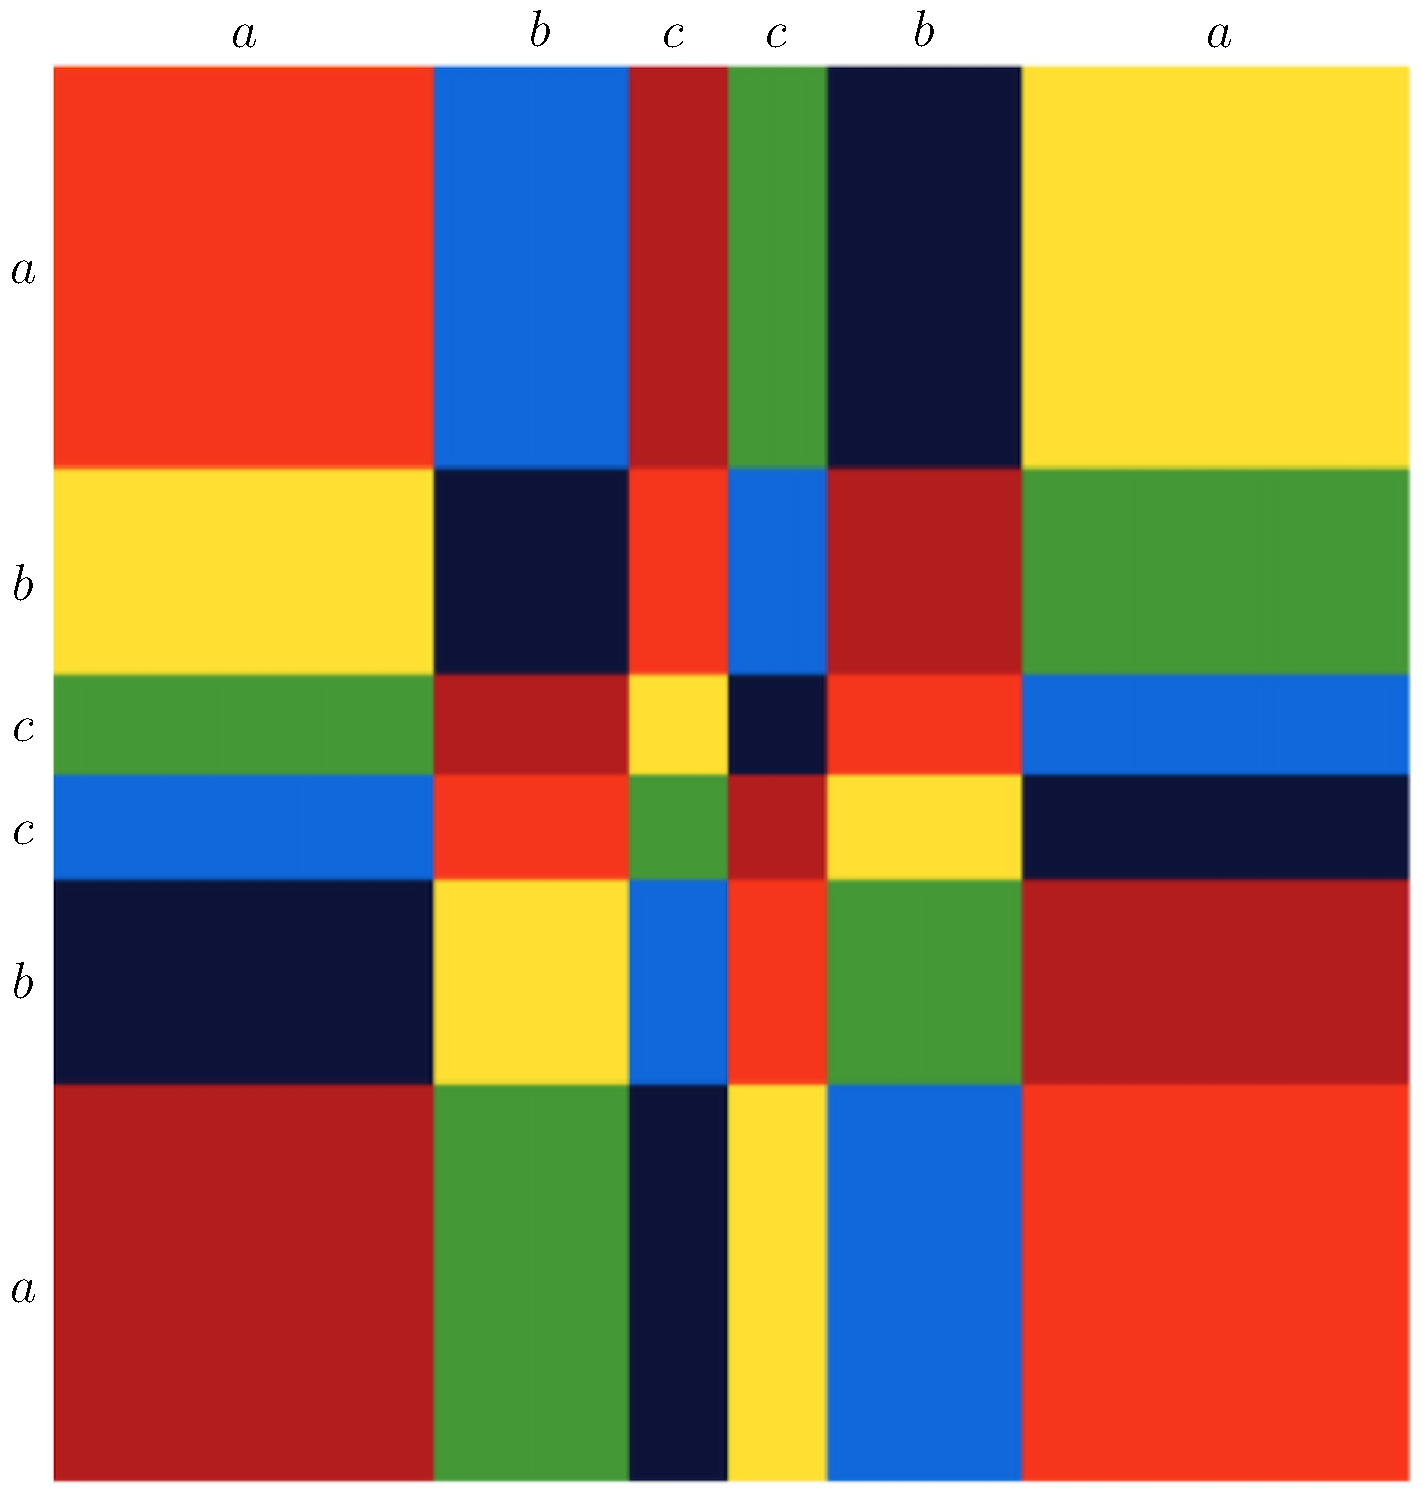
\includegraphics[width=0.3\textwidth]{pics/Lohse2}
 \end{center} }
        \solution{ }
        \end{Add}
        \begin{Add}{ScM}{basal1}{Mathematisieren}{mittel}
        \question{ Beschreibe alle grünen Flächen mit einem Term (z.B. ist die Fläche des oranges Quadrats oben links $a^2$.) und vereinfache diesen soweit als möglich.
\begin{center}
 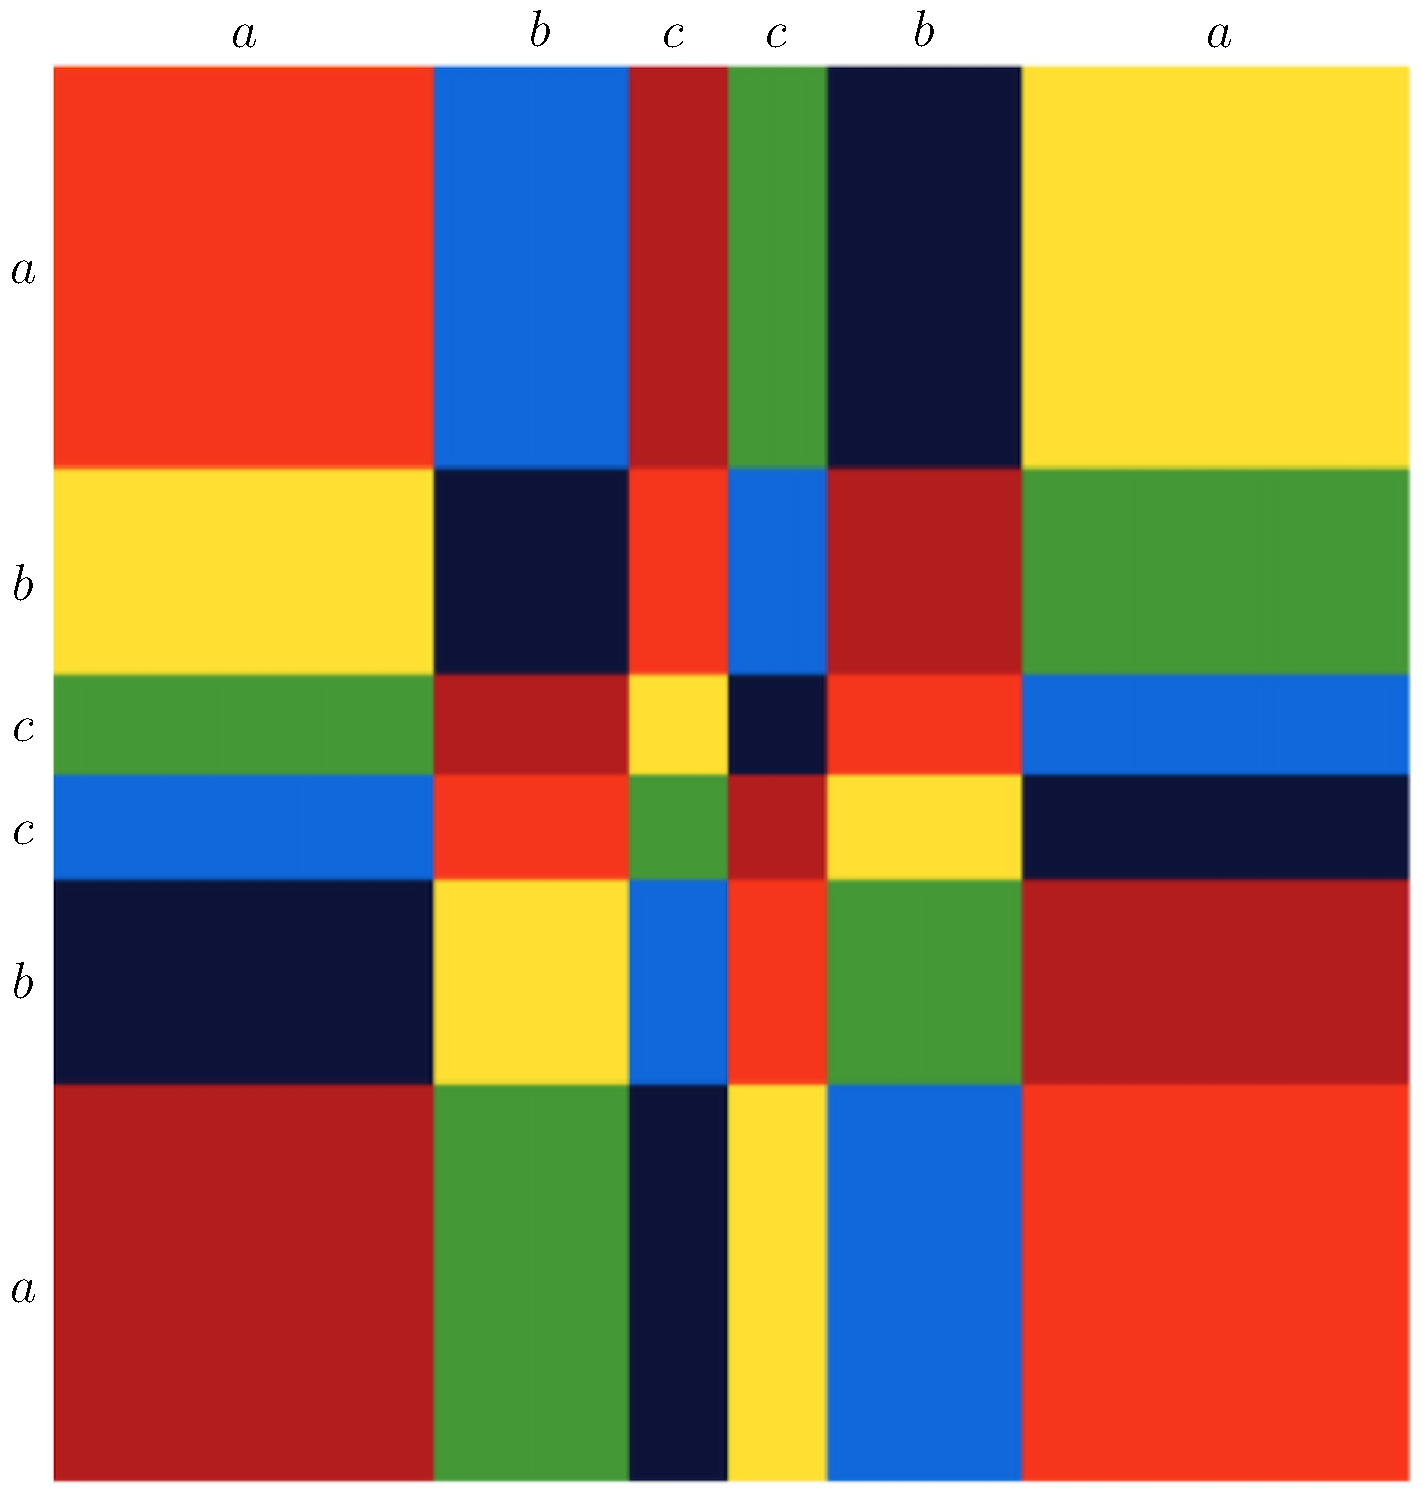
\includegraphics[width=0.3\textwidth]{pics/Lohse2}
 \end{center} }
        \solution{ $2ab+2ac+b^2+c^2$ }
        \end{Add}
        

\begin{Add}{WaJ}{basal1}{Potenzen}{mittel}
\question{ $$2\cdot10^5\cdot7\cdot10^9=\;?$$ }
\solution{ }
\end{Add}
\begin{Add}{WaJ}{basal1}{Potenzen}{mittel}
\question{ $$2\cdot10^5\cdot7\cdot10^9=\;?$$ }
\solution{ $14\cdot10^{14}=1.4\cdot10^{15}$ }
\end{Add}

\begin{Add}{WaJ}{basal1}{Bruchrechnen}{mittel}
\question{ $$\frac{2}{3}-\frac{5}{7}=\;?$$ }
\solution{ }
\end{Add}
\begin{Add}{WaJ}{basal1}{Bruchrechnen}{mittel}
\question{ $$\frac{2}{3}-\frac{5}{7}=\;?$$ }
\solution{ $-\frac{1}{21}$ }
\end{Add}

\begin{Add}{WaJ}{basal2}{Potenzen}{mittel}
\question{ $$\sqrt{4\cdot10^{12}}=\;?$$ }
\solution{ }
\end{Add}
\begin{Add}{WaJ}{basal2}{Potenzen}{mittel}
\question{ $$\sqrt{4\cdot10^{12}}=\;?$$ }
\solution{ $2\cdot10^6$ }
\end{Add}

\begin{Add}{WaJ}{basal2}{Bruchrechnen}{schwer}
\question{ $$\frac{2x}{\frac{4x}{5}}=\;?$$ }
\solution{ }
\end{Add}
\begin{Add}{WaJ}{basal2}{Bruchrechnen}{schwer}
\question{ $$\frac{2x}{\frac{4x}{5}}=\;?$$ }
\solution{ $\frac{5}{2}$ }
\end{Add}

    \begin{Add}{WaJ}{basal2}{Bruchgleichungen}{mittel}
    \question{ Löse nach $x$:
$$-\frac{3}{7}x+5=2$$ }
    \solution{ }
    \end{Add}
    \begin{Add}{WaJ}{basal2}{Bruchgleichungen}{mittel}
    \question{ Löse nach $x$:
$$-\frac{3}{7}x+5=2$$ }
    \solution{ $x=7$ }
    \end{Add}
    

\begin{Add}{WaJ}{basal1}{Einheiten}{leicht}
\question{ $$\unitfrac[72]{km}{h}=\unitfrac[\;?]{m}{s}$$ }
\solution{ }
\end{Add}
\begin{Add}{WaJ}{basal1}{Einheiten}{leicht}
\question{ $$\unitfrac[72]{km}{h}=\unitfrac[\;?]{m}{s}$$ }
\solution{ $\unitfrac[20]{m}{s}$ }
\end{Add}

\begin{Add}{WaJ}{basal1}{Einheiten}{leicht}
\question{ $$\unit[200]{Liter}=\unit[\;?]{m^3}$$ }
\solution{ }
\end{Add}
\begin{Add}{WaJ}{basal1}{Einheiten}{leicht}
\question{ $$\unit[200]{Liter}=\unit[\;?]{m^3}$$ }
\solution{ $\unit[0.2]{m^3}$ }
\end{Add}

    \begin{Add}{WaJ}{basal2}{Funktionsauswertung}{leicht}
    \question{ Sei $f(x)=\frac{1}{2}x-1$. Bestimme
$$f(-3)$$ }
    \solution{ }
    \end{Add}
    \begin{Add}{WaJ}{basal2}{Funktionsauswertung}{leicht}
    \question{ Sei $f(x)=\frac{1}{2}x-1$. Bestimme
$$f(-3)$$ }
    \solution{ $f(-3)=-\frac{5}{2}$ }
    \end{Add}
    

    \begin{Add}{WaJ}{basal2}{Funktionsauswertung}{leicht}
    \question{ Sei $f(x)=x^2$. Bestimme
$$f(-2)$$ }
    \solution{ }
    \end{Add}
    \begin{Add}{WaJ}{basal2}{Funktionsauswertung}{leicht}
    \question{ Sei $f(x)=x^2$. Bestimme
$$f(-2)$$ }
    \solution{ $f(-2)=4$ }
    \end{Add}
    

    \begin{Add}{WaJ}{basal1}{BinomischeFormeln,Grundoperationen}{mittel}
    \question{ Faktorisiere
$$x^2-2x+1$$ }
    \solution{ }
    \end{Add}
    \begin{Add}{WaJ}{basal1}{BinomischeFormeln,Grundoperationen}{mittel}
    \question{ Faktorisiere
$$x^2-2x+1$$ }
    \solution{ $(x-1)^2$ }
    \end{Add}
    

\begin{Add}{WaJ}{basal1}{BinomischeFormeln,Grundoperationen}{leicht}
\question{ $$\left(2-\sqrt{2}\right)\left(2+\sqrt{2}\right)=\;?$$ }
\solution{ }
\end{Add}
\begin{Add}{WaJ}{basal1}{BinomischeFormeln,Grundoperationen}{leicht}
\question{ $$\left(2-\sqrt{2}\right)\left(2+\sqrt{2}\right)=\;?$$ }
\solution{ $2$ }
\end{Add}

    \begin{Add}{WaJ}{basal1}{Pythagoras}{leicht}
    \question{ Gegeben seien die Katheten $a=\unit[4]{m}$ und $b=\unit[3]{m}$. 
Wie lang ist die Seite $c$?
\begin{center}
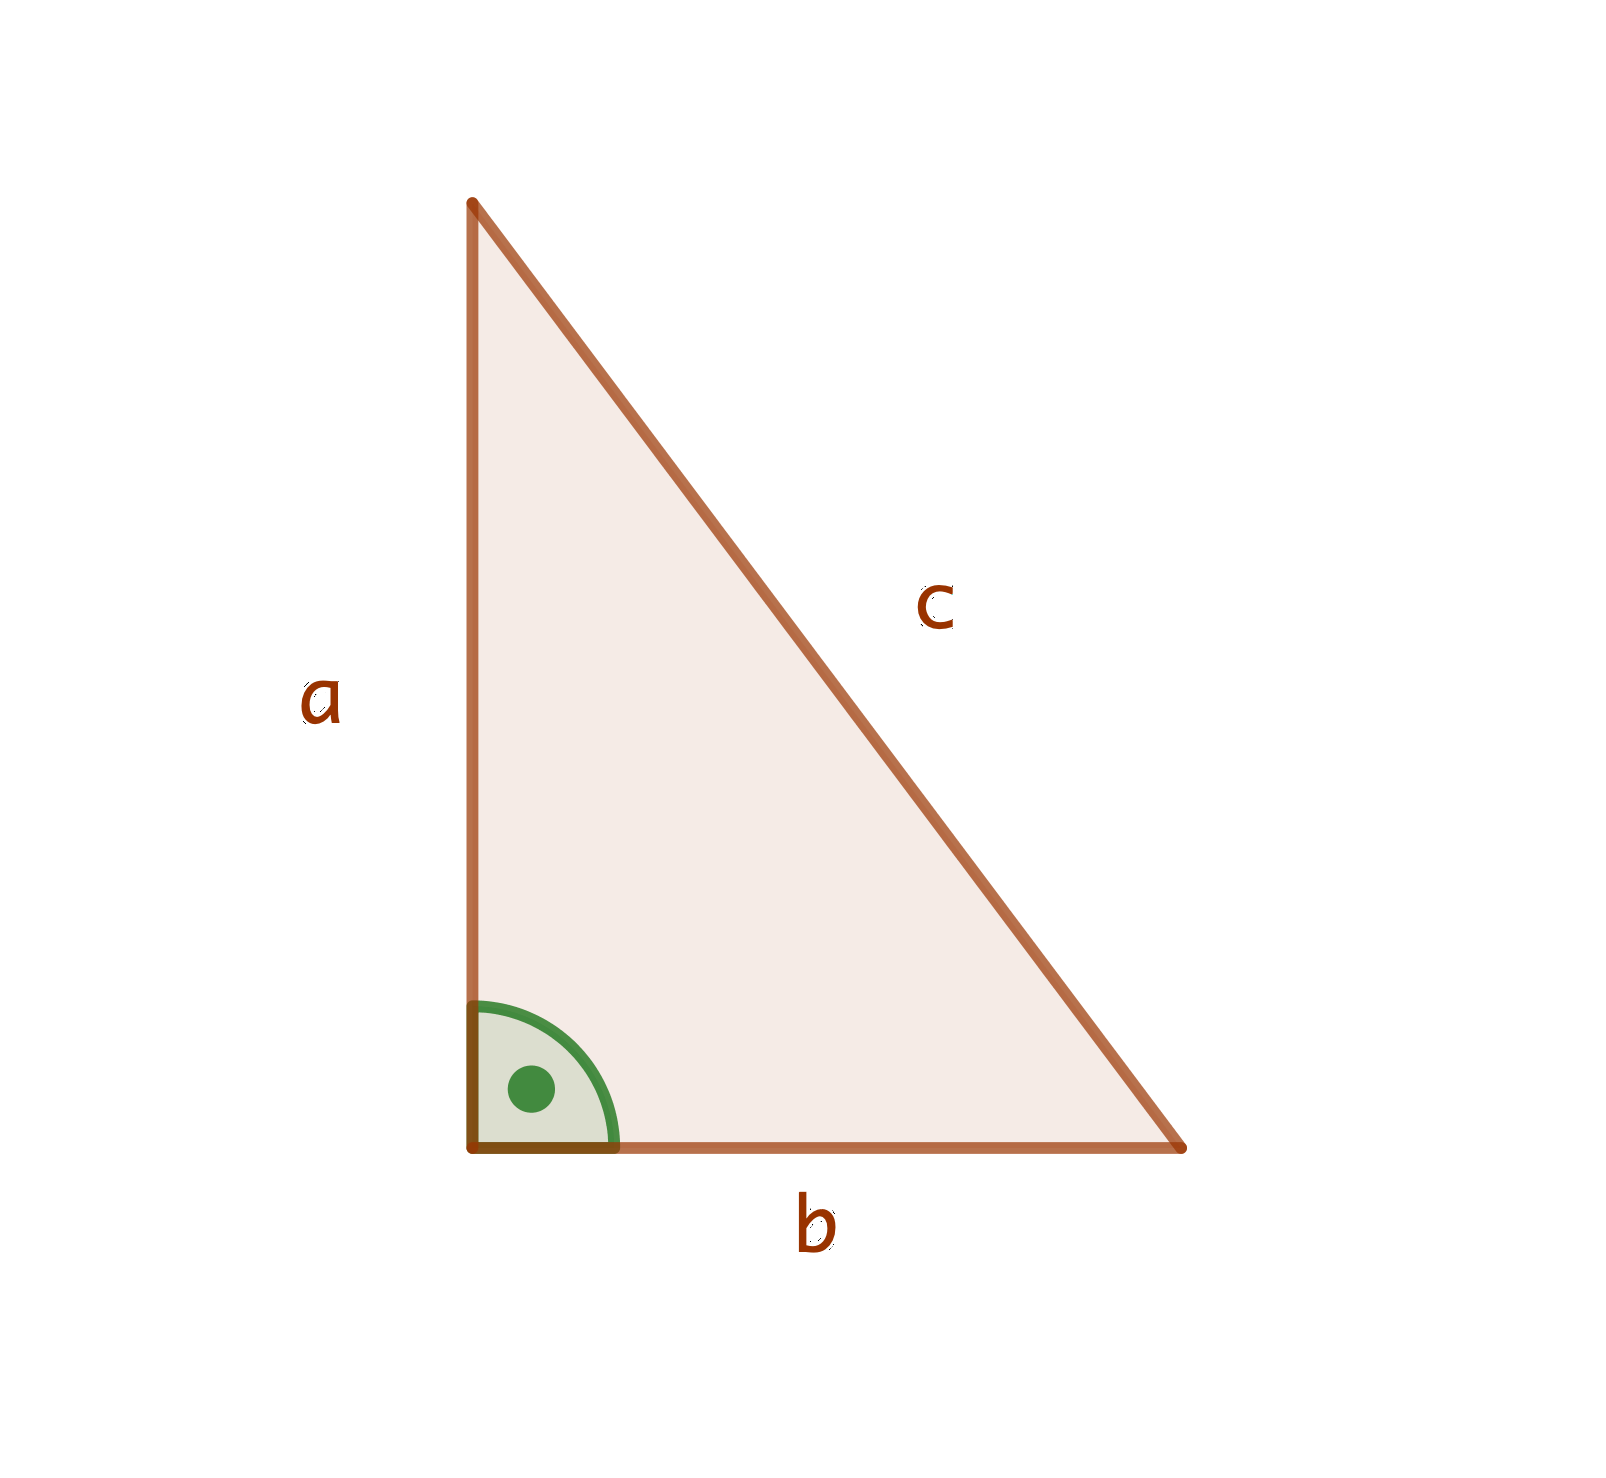
\includegraphics[width=0.382\textwidth]{pics/wajpythagoras.png}
\end{center} }
    \solution{ }
    \end{Add}
    \begin{Add}{WaJ}{basal1}{Pythagoras}{leicht}
    \question{ Gegeben seien die Katheten $a=\unit[4]{m}$ und $b=\unit[3]{m}$. 
Wie lang ist die Seite $c$?
\begin{center}
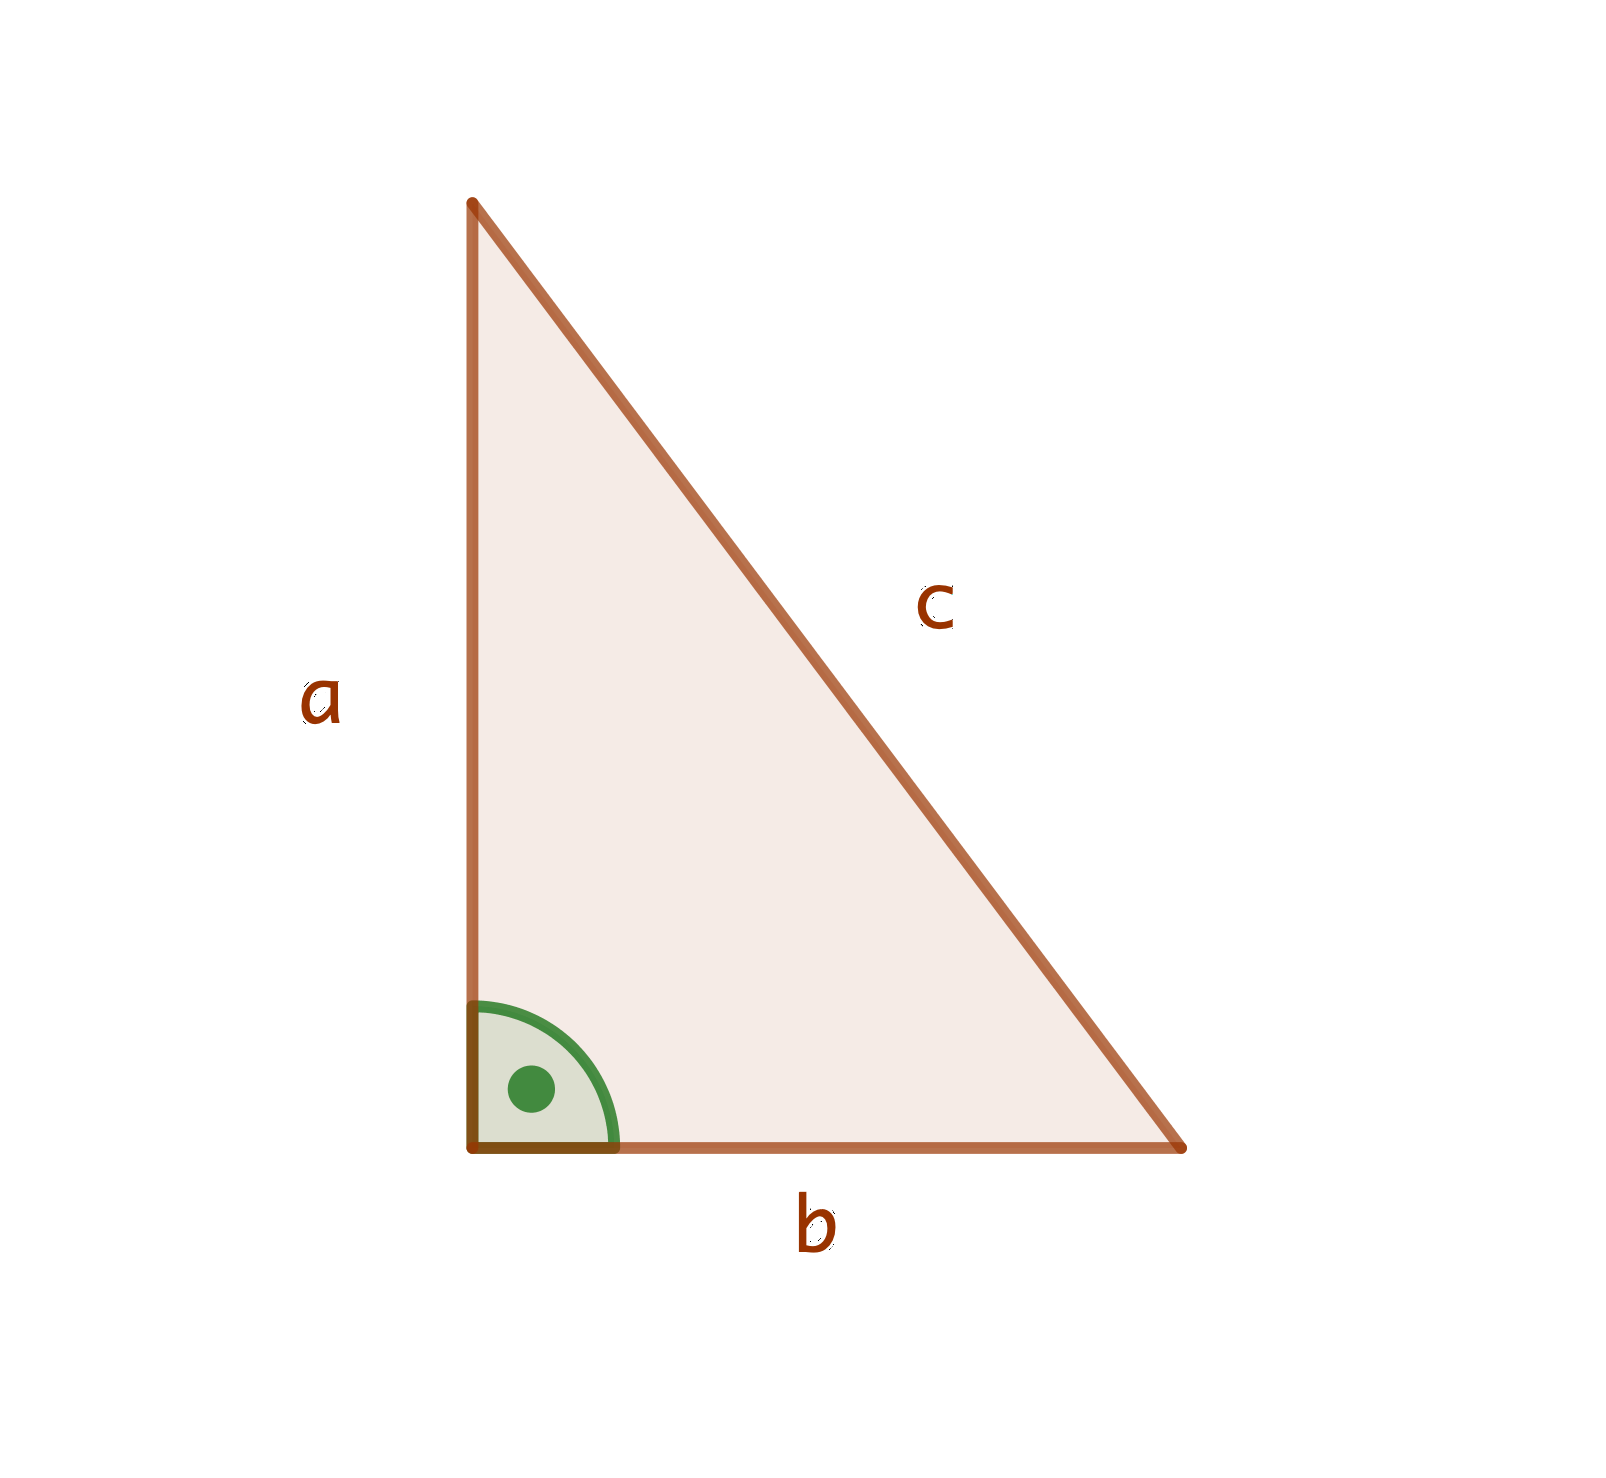
\includegraphics[width=0.382\textwidth]{pics/wajpythagoras.png}
\end{center} }
    \solution{ $c=\unit[5]{m}$ }
    \end{Add}
    

    \begin{Add}{WaJ}{basal1}{Pythagoras}{mittel}
    \question{ Gegeben seien die Kathete $a=\unit[4]{m}$ und die Hypotenuse $c=\unit[5]{m}$. 
Wie lang ist die Seite $b$?
\begin{center}
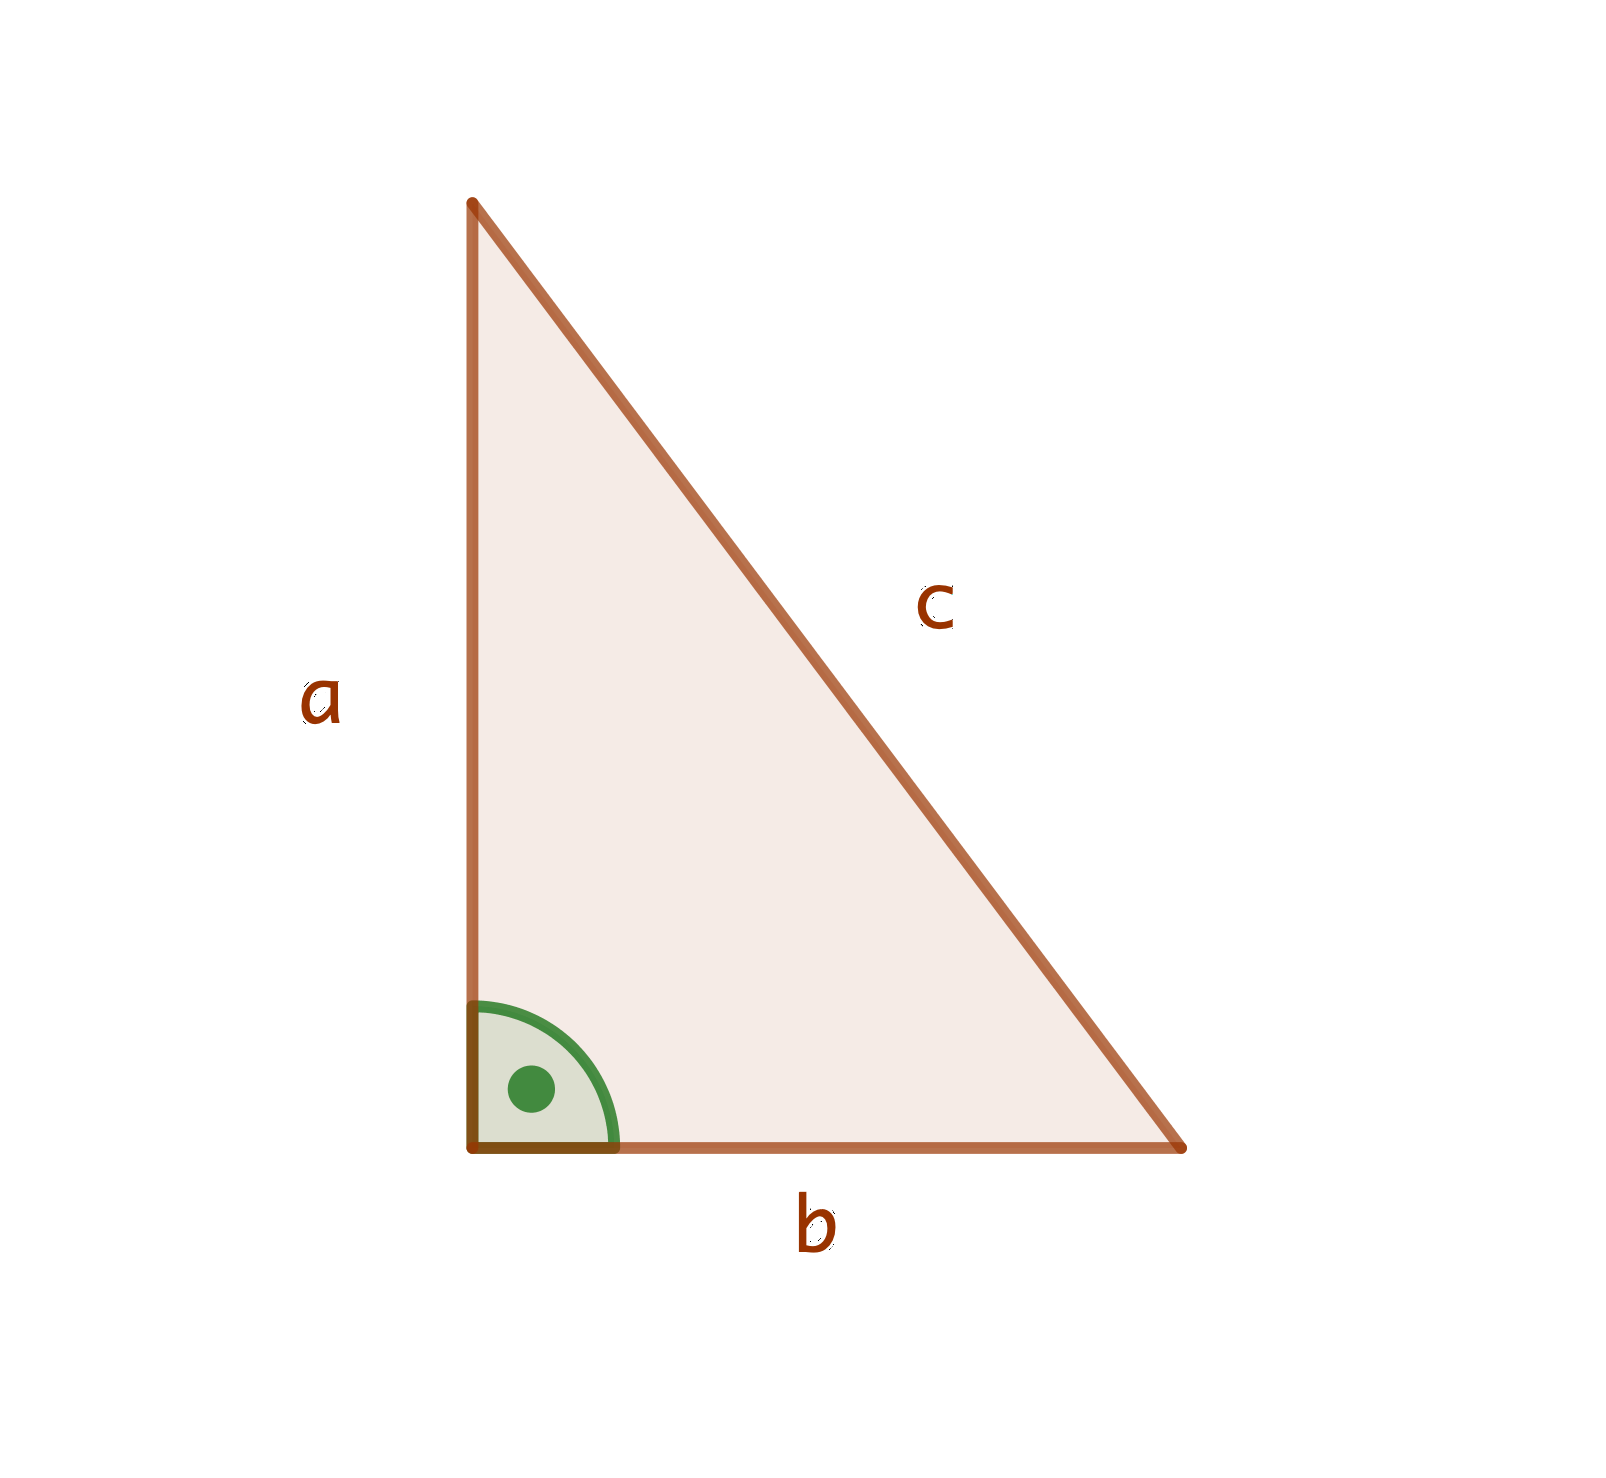
\includegraphics[width=0.382\textwidth]{pics/wajpythagoras.png}
\end{center} }
    \solution{ }
    \end{Add}
    \begin{Add}{WaJ}{basal1}{Pythagoras}{mittel}
    \question{ Gegeben seien die Kathete $a=\unit[4]{m}$ und die Hypotenuse $c=\unit[5]{m}$. 
Wie lang ist die Seite $b$?
\begin{center}
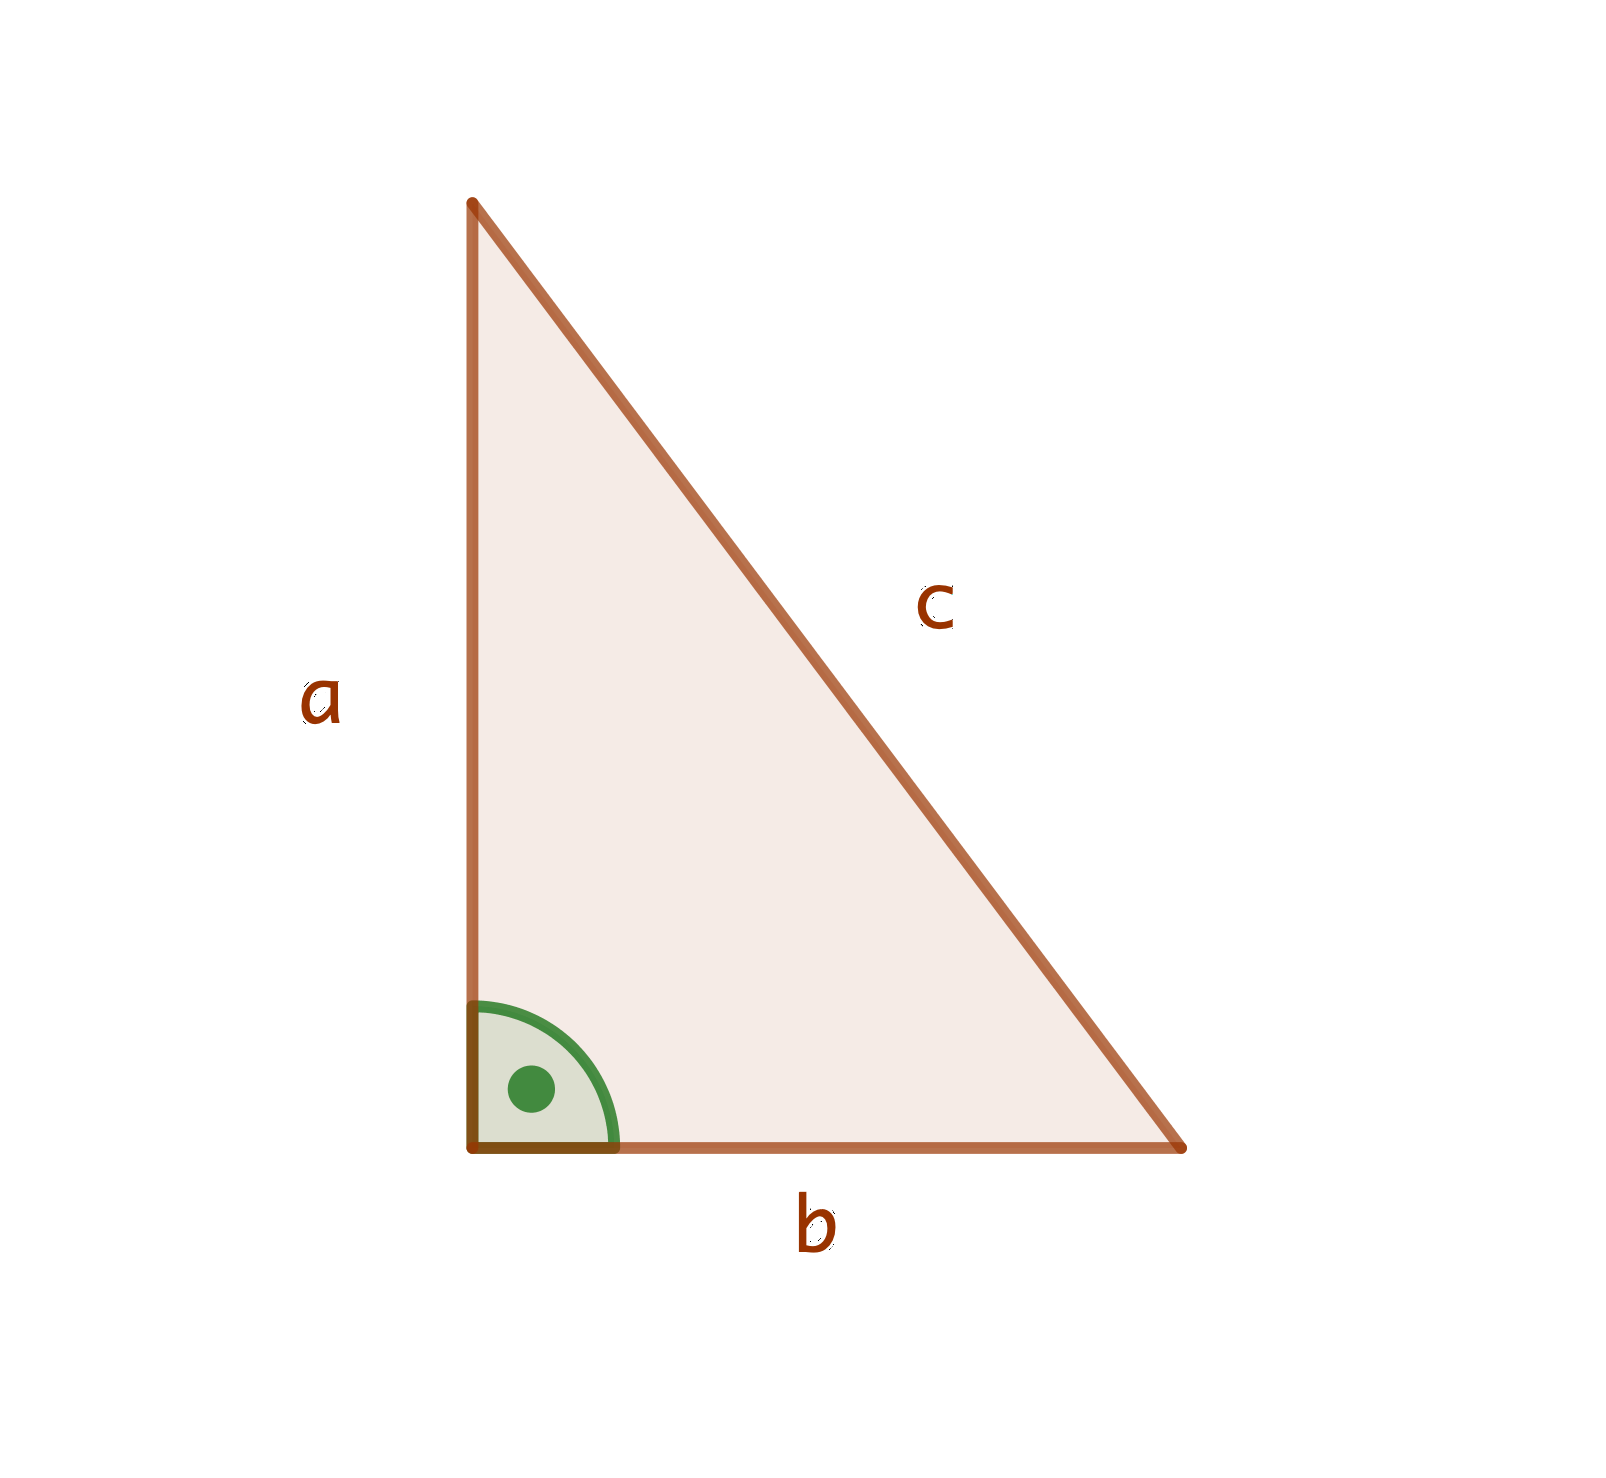
\includegraphics[width=0.382\textwidth]{pics/wajpythagoras.png}
\end{center} }
    \solution{ $c=\unit[3]{m}$ }
    \end{Add}
    

\begin{Add}{WaJ}{basal1}{Proportionalitäten}{mittel}
\question{ Wie viel sind $\unit[80]{\%}$ von $\unit[80]{\%}$ von $200$. }
\solution{ }
\end{Add}
\begin{Add}{WaJ}{basal1}{Proportionalitäten}{mittel}
\question{ Wie viel sind $\unit[80]{\%}$ von $\unit[80]{\%}$ von $200$. }
\solution{ $128$ }
\end{Add}

\begin{Add}{WaJ}{basal1}{Kreisberechnung}{leicht}
\question{ Wie lang ist der Umfang eines Kreises mit Radius $\unit[2]{m}$? }
\solution{ }
\end{Add}
\begin{Add}{WaJ}{basal1}{Kreisberechnung}{leicht}
\question{ Wie lang ist der Umfang eines Kreises mit Radius $\unit[2]{m}$? }
\solution{ $\unit[4\pi]{m}$ }
\end{Add}

\begin{Add}{WaJ}{basal1}{Kreisberechnung}{leicht}
\question{ Wie gross ist die Fläche eines Kreises mit Radius $\unit[2]{m}$? }
\solution{ }
\end{Add}
\begin{Add}{WaJ}{basal1}{Kreisberechnung}{leicht}
\question{ Wie gross ist die Fläche eines Kreises mit Radius $\unit[2]{m}$? }
\solution{ $\unit[4\pi]{m^2}$ }
\end{Add}

\begin{Add}{WaJ}{basal1}{Kreisberechnung}{mittel}
\question{ Wie gross ist die Fläche eines Kreises mit Durchmesser $\unit[1.6]{m}$? }
\solution{ }
\end{Add}
\begin{Add}{WaJ}{basal1}{Kreisberechnung}{mittel}
\question{ Wie gross ist die Fläche eines Kreises mit Durchmesser $\unit[1.6]{m}$? }
\solution{ $\unit[\frac{16}{25}\pi]{m^2}$ }
\end{Add}

\begin{Add}{WaJ}{basal1}{Kreisberechnung}{schwer}
\question{ Wie gross ist der Durchmesser eines Kreises mit Flä\-chen\-in\-halt $\unit[\frac{9\pi}{4}]{m^2}$? }
\solution{ }
\end{Add}
\begin{Add}{WaJ}{basal1}{Kreisberechnung}{schwer}
\question{ Wie gross ist der Durchmesser eines Kreises mit Flä\-chen\-in\-halt $\unit[\frac{9\pi}{4}]{m^2}$? }
\solution{ $\unit[3]{m}$ }
\end{Add}

\begin{Add}{WaJ}{basal1}{Termumformungen}{leicht}
\question{ $$2a-(4+a)=\;?$$ }
\solution{ }
\end{Add}
\begin{Add}{WaJ}{basal1}{Termumformungen}{leicht}
\question{ $$2a-(4+a)=\;?$$ }
\solution{ $a-4$ }
\end{Add}

\begin{Add}{WaJ}{basal1}{Termumformungen}{mittel}
\question{ $$2a-(4+a)\cdot(-2)=\;?$$ }
\solution{ }
\end{Add}
\begin{Add}{WaJ}{basal1}{Termumformungen}{mittel}
\question{ $$2a-(4+a)\cdot(-2)=\;?$$ }
\solution{ $4(a+2)$ }
\end{Add}

\begin{Add}{WaJ}{basal1}{Termumformungen}{mittel}
\question{ $$(-2)\cdot(-3)^2=\;?$$ }
\solution{ }
\end{Add}
\begin{Add}{WaJ}{basal1}{Termumformungen}{mittel}
\question{ $$(-2)\cdot(-3)^2=\;?$$ }
\solution{ $-18$ }
\end{Add}

\begin{Add}{WaJ}{basal1}{Termumformungen}{leicht}
\question{ $$xy+x+y-yx=\;?$$ }
\solution{ }
\end{Add}
\begin{Add}{WaJ}{basal1}{Termumformungen}{leicht}
\question{ $$xy+x+y-yx=\;?$$ }
\solution{ $x+y$ }
\end{Add}

\begin{Add}{WaJ}{basal1}{Termumformungen}{leicht}
\question{ $$3-\frac{7}{5}=\;?$$ }
\solution{ }
\end{Add}
\begin{Add}{WaJ}{basal1}{Termumformungen}{leicht}
\question{ $$3-\frac{7}{5}=\;?$$ }
\solution{ $\frac{8}{5}$ }
\end{Add}

\begin{Add}{WaJ}{basal1}{Termumformungen}{schwer}
\question{ $$\left(1-3\cdot\left(-\frac{7}{6}\right)\right)^2=\;?$$ }
\solution{ }
\end{Add}
\begin{Add}{WaJ}{basal1}{Termumformungen}{schwer}
\question{ $$\left(1-3\cdot\left(-\frac{7}{6}\right)\right)^2=\;?$$ }
\solution{ $\frac{81}{4}$ }
\end{Add}

\begin{Add}{WaJ}{basal1}{Bruchrechnen}{leicht}
\question{ $$\frac{2}{3}+\frac{2}{3}=\;?$$ }
\solution{ }
\end{Add}
\begin{Add}{WaJ}{basal1}{Bruchrechnen}{leicht}
\question{ $$\frac{2}{3}+\frac{2}{3}=\;?$$ }
\solution{ $\frac{4}{3}$ }
\end{Add}

\begin{Add}{WaJ}{basal1}{Bruchrechnen}{leicht}
\question{ $$\frac{2}{3}+\frac{3}{2}=\;?$$ }
\solution{ }
\end{Add}
\begin{Add}{WaJ}{basal1}{Bruchrechnen}{leicht}
\question{ $$\frac{2}{3}+\frac{3}{2}=\;?$$ }
\solution{ $\frac{13}{6}$ }
\end{Add}

\begin{Add}{WaJ}{basal1}{Bruchrechnen}{mittel}
\question{ $$\frac{2}{-3}+\frac{3}{2}\cdot\frac{4}{9}=\;?$$ }
\solution{ }
\end{Add}
\begin{Add}{WaJ}{basal1}{Bruchrechnen}{mittel}
\question{ $$\frac{2}{-3}+\frac{3}{2}\cdot\frac{4}{9}=\;?$$ }
\solution{ $0$ }
\end{Add}

\begin{Add}{WaJ}{basal1}{Bruchrechnen}{schwer}
\question{ $$\frac{\frac{4}{3}}{\frac{1}{2}}-\frac{3}{7}\cdot\frac{35}{9}=\;?$$ }
\solution{ }
\end{Add}
\begin{Add}{WaJ}{basal1}{Bruchrechnen}{schwer}
\question{ $$\frac{\frac{4}{3}}{\frac{1}{2}}-\frac{3}{7}\cdot\frac{35}{9}=\;?$$ }
\solution{ $1$ }
\end{Add}

    \begin{Add}{GiD}{basal1}{Bruchrechnen}{leicht}
    \question{ Vereinfache den gewöhnlichen Bruch so weit wie möglich.
$$\frac{5}{6}+\frac{2}{5}=\;?$$
$$\frac{5}{6}\cdot\frac{2}{5}=\;?$$ }
    \solution{ }
    \end{Add}
    \begin{Add}{GiD}{basal1}{Bruchrechnen}{leicht}
    \question{ Vereinfache den gewöhnlichen Bruch so weit wie möglich.
$$\frac{5}{6}+\frac{2}{5}=\;?$$
$$\frac{5}{6}\cdot\frac{2}{5}=\;?$$ }
    \solution{ $\frac{37}{30}=1\frac{7}{30} ; \frac{1}{3}$ }
    \end{Add}
    

\begin{Add}{WaJ}{basal1}{Termumformungen}{mittel}
\question{ $$4-2^4\cdot3=\;?$$ }
\solution{ }
\end{Add}
\begin{Add}{WaJ}{basal1}{Termumformungen}{mittel}
\question{ $$4-2^4\cdot3=\;?$$ }
\solution{ $-44$ }
\end{Add}

\begin{Add}{WaJ}{basal1}{Termumformungen}{mittel}
\question{ $$4-3\cdot(-2)^3=\;?$$ }
\solution{ }
\end{Add}
\begin{Add}{WaJ}{basal1}{Termumformungen}{mittel}
\question{ $$4-3\cdot(-2)^3=\;?$$ }
\solution{ $28$ }
\end{Add}

\begin{Add}{WaJ}{basal1}{Dreieck}{leicht}
\question{ In einem gleichseitigen Dreieck betragen die Winkel \dots$^\circ$ }
\solution{ }
\end{Add}
\begin{Add}{WaJ}{basal1}{Dreieck}{leicht}
\question{ In einem gleichseitigen Dreieck betragen die Winkel \dots$^\circ$ }
\solution{ $60^\circ$ }
\end{Add}

\begin{Add}{WaJ}{basal1}{Dreieck}{leicht}
\question{ In einem rechtwinkligen, gleichschenkligen Dreieck betragen die Basiswinkel \dots$^\circ$ }
\solution{ }
\end{Add}
\begin{Add}{WaJ}{basal1}{Dreieck}{leicht}
\question{ In einem rechtwinkligen, gleichschenkligen Dreieck betragen die Basiswinkel \dots$^\circ$ }
\solution{ $45^\circ$ }
\end{Add}

\begin{Add}{WaJ}{basal1}{Dreieck}{mittel}
\question{ In einem gleichschenkligen, rechtwinkligen Dreieck mit Kathetenlängen jeweils $1$ beträgt die Hypotenuse \dots }
\solution{ }
\end{Add}
\begin{Add}{WaJ}{basal1}{Dreieck}{mittel}
\question{ In einem gleichschenkligen, rechtwinkligen Dreieck mit Kathetenlängen jeweils $1$ beträgt die Hypotenuse \dots }
\solution{ $\sqrt{2}$ }
\end{Add}

\begin{Add}{WaJ}{basal1}{Dreieck}{mittel}
\question{ Wenn in einem rechtwinkligen Dreieck die Hypotenuse $3$ und eine Kathete $2$ lang ist, dann ist die andere Kathete \dots\ lang. }
\solution{ }
\end{Add}
\begin{Add}{WaJ}{basal1}{Dreieck}{mittel}
\question{ Wenn in einem rechtwinkligen Dreieck die Hypotenuse $3$ und eine Kathete $2$ lang ist, dann ist die andere Kathete \dots\ lang. }
\solution{ $\sqrt{5}$ }
\end{Add}

\begin{Add}{WaJ}{basal1}{Dreieck}{schwer}
\question{ In einem gleichseitigen Dreieck betrage die Höhe $\sqrt{3}$. Wie lang ist eine Seite? }
\solution{ }
\end{Add}
\begin{Add}{WaJ}{basal1}{Dreieck}{schwer}
\question{ In einem gleichseitigen Dreieck betrage die Höhe $\sqrt{3}$. Wie lang ist eine Seite? }
\solution{ $2$ }
\end{Add}

\begin{Add}{RoK}{basal1}{Dreieck,Proportionalitäten,Mathematisieren}{mittel}
\question{ Die drei Innenwinkel eines Dreiecks verhalten sich wie $7:8:9$. Wie gross sind die drei Winkel? }
\solution{ }
\end{Add}
\begin{Add}{RoK}{basal1}{Dreieck,Proportionalitäten,Mathematisieren}{mittel}
\question{ Die drei Innenwinkel eines Dreiecks verhalten sich wie $7:8:9$. Wie gross sind die drei Winkel? }
\solution{ $105^\circ$, $120^\circ$ und $135^\circ$ }
\end{Add}

\begin{Add}{RoK}{basal2}{Mathematisieren}{mittel}
\question{ Wird auf beiden Seiten einer zweistelligen natürlichen Zahl die Ziffer 5 hinzugefügt, so ergibt sich das 75-fache der Zahl. wie heisst die Zahl? }
\solution{ }
\end{Add}
\begin{Add}{RoK}{basal2}{Mathematisieren}{mittel}
\question{ Wird auf beiden Seiten einer zweistelligen natürlichen Zahl die Ziffer 5 hinzugefügt, so ergibt sich das 75-fache der Zahl. wie heisst die Zahl? }
\solution{ $\frac{1001}{13}=77$ }
\end{Add}

    \begin{Add}{RoK}{basal2}{Potenzen}{mittel}
    \question{ Löse die Gleichung nach $x$ auf:
$$5^x=5\cdot 5^{20}+20\cdot 5^{20}$$ }
    \solution{ }
    \end{Add}
    \begin{Add}{RoK}{basal2}{Potenzen}{mittel}
    \question{ Löse die Gleichung nach $x$ auf:
$$5^x=5\cdot 5^{20}+20\cdot 5^{20}$$ }
    \solution{ $x=22$ }
    \end{Add}
    

    \begin{Add}{RoK}{basal2}{Potenzen}{schwer}
    \question{ Löse die Gleichung nach $x$ auf:
$$2\cdot 4^x-24\cdot 4^{32}=8\cdot 4^{32}$$ }
    \solution{ }
    \end{Add}
    \begin{Add}{RoK}{basal2}{Potenzen}{schwer}
    \question{ Löse die Gleichung nach $x$ auf:
$$2\cdot 4^x-24\cdot 4^{32}=8\cdot 4^{32}$$ }
    \solution{ $x=34$ }
    \end{Add}
    

\begin{Add}{RoK}{basal1}{Bruchrechnen}{leicht}
\question{ Welche Zahl liegt auf der Zahlengerade exakt zwischen $-\frac{2}{3}$ und $\frac{1}{5}$? }
\solution{ }
\end{Add}
\begin{Add}{RoK}{basal1}{Bruchrechnen}{leicht}
\question{ Welche Zahl liegt auf der Zahlengerade exakt zwischen $-\frac{2}{3}$ und $\frac{1}{5}$? }
\solution{ $-\frac{7}{30}$ }
\end{Add}

\begin{Add}{RoK}{basal1}{Begrifflichkeiten}{leicht}
\question{ Berechne das kgV und den ggT der Zahlen 14 und 35. }
\solution{ }
\end{Add}
\begin{Add}{RoK}{basal1}{Begrifflichkeiten}{leicht}
\question{ Berechne das kgV und den ggT der Zahlen 14 und 35. }
\solution{ $kgV(14,35)=70,~ggT(14,35)=7$ }
\end{Add}

\begin{Add}{RoK}{basal1}{Begrifflichkeiten}{leicht}
\question{ Der Term ist ein Quotient. Der Dividend ist die Differenz aus $x$ und $y$, der Divisor ist die Summe aus 2 und $z$. Wie lautet der Term? }
\solution{ }
\end{Add}
\begin{Add}{RoK}{basal1}{Begrifflichkeiten}{leicht}
\question{ Der Term ist ein Quotient. Der Dividend ist die Differenz aus $x$ und $y$, der Divisor ist die Summe aus 2 und $z$. Wie lautet der Term? }
\solution{ $\frac{x-y}{2+z}$ }
\end{Add}

\begin{Add}{RoK}{basal1}{Begrifflichkeiten}{leicht}
\question{ Berechne das kgV und den ggT der Zahlen 45 und 75. }
\solution{ }
\end{Add}
\begin{Add}{RoK}{basal1}{Begrifflichkeiten}{leicht}
\question{ Berechne das kgV und den ggT der Zahlen 45 und 75. }
\solution{ $kgV(14,35)=225,~ggT(14,35)=15$ }
\end{Add}

    \begin{Add}{RoK}{basal1}{Begrifflichkeiten}{leicht}
    \question{ Ordne nach aufsteigender Grösse:
$$\pi,~\frac{16}{5},~\sqrt{13},~2^2,~\frac{28}{9},~\sqrt{\sqrt{81}}$$ }
    \solution{ }
    \end{Add}
    \begin{Add}{RoK}{basal1}{Begrifflichkeiten}{leicht}
    \question{ Ordne nach aufsteigender Grösse:
$$\pi,~\frac{16}{5},~\sqrt{13},~2^2,~\frac{28}{9},~\sqrt{\sqrt{81}}$$ }
    \solution{ $\sqrt{\sqrt{81}},~\frac{28}{9},~\pi,~\frac{16}{5},~\sqrt{13},~2^2$ }
    \end{Add}
    

\begin{Add}{RoK}{basal1}{Einheiten,Potenzen}{leicht}
\question{ $20~m^2$ entsprechen $2\cdot 10^x~mm^2$. }
\solution{ }
\end{Add}
\begin{Add}{RoK}{basal1}{Einheiten,Potenzen}{leicht}
\question{ $20~m^2$ entsprechen $2\cdot 10^x~mm^2$. }
\solution{ $x=7$ }
\end{Add}

\begin{Add}{RoK}{basal1}{Einheiten}{leicht}
\question{ Auf einem Fussballfeld mit den Massen 100 mal 50 Meter steht das Wasser 1 cm hoch. Wie viele Liter Wasser sind das? }
\solution{ }
\end{Add}
\begin{Add}{RoK}{basal1}{Einheiten}{leicht}
\question{ Auf einem Fussballfeld mit den Massen 100 mal 50 Meter steht das Wasser 1 cm hoch. Wie viele Liter Wasser sind das? }
\solution{ 50'000 Liter }
\end{Add}

\begin{Add}{RoK}{basal1}{Einheiten}{leicht}
\question{ Ein Aquarium hat eine Breite von 80 cm, eine Tiefe von 40 cm und eine Höhe von 50 cm. Wie viele Liter passen maximal in das Aquarium? }
\solution{ }
\end{Add}
\begin{Add}{RoK}{basal1}{Einheiten}{leicht}
\question{ Ein Aquarium hat eine Breite von 80 cm, eine Tiefe von 40 cm und eine Höhe von 50 cm. Wie viele Liter passen maximal in das Aquarium? }
\solution{ 160 Liter }
\end{Add}

\begin{Add}{RoK}{basal1}{Einheiten}{leicht}
\question{ Ein Quader mit quadratischer Grundfläche und der Höhe 40 cm soll ein Volumen von einem Liter haben. Welche Masse hat die Grundfläche? }
\solution{ }
\end{Add}
\begin{Add}{RoK}{basal1}{Einheiten}{leicht}
\question{ Ein Quader mit quadratischer Grundfläche und der Höhe 40 cm soll ein Volumen von einem Liter haben. Welche Masse hat die Grundfläche? }
\solution{ Das Grundquadrat hat eine Seitenlänge von 5 cm }
\end{Add}

\begin{Add}{RoK}{basal1}{Bruchgleichungen}{leicht}
\question{ $$\frac{10+x}{18}=\frac{10-x}{12}$$ }
\solution{ }
\end{Add}
\begin{Add}{RoK}{basal1}{Bruchgleichungen}{leicht}
\question{ $$\frac{10+x}{18}=\frac{10-x}{12}$$ }
\solution{ $x=2$ }
\end{Add}

\begin{Add}{RoK}{basal1}{Bruchrechnen}{leicht}
\question{ $$\frac{1}{1}+\frac{1}{2}+\frac{1}{3}+\frac{1}{4}=$$ }
\solution{ }
\end{Add}
\begin{Add}{RoK}{basal1}{Bruchrechnen}{leicht}
\question{ $$\frac{1}{1}+\frac{1}{2}+\frac{1}{3}+\frac{1}{4}=$$ }
\solution{ $\frac{25}{12}$ }
\end{Add}

\begin{Add}{RoK}{basal1}{Kreisberechnung}{leicht}
\question{ Ein Velorad hat einen Durchmesser von 28 Zoll. Ein Zoll entspricht 2.54 cm. Wie weit fährt das Velo mit einer Radumdrehung? }
\solution{ }
\end{Add}
\begin{Add}{RoK}{basal1}{Kreisberechnung}{leicht}
\question{ Ein Velorad hat einen Durchmesser von 28 Zoll. Ein Zoll entspricht 2.54 cm. Wie weit fährt das Velo mit einer Radumdrehung? }
\solution{ 223.43 cm }
\end{Add}

\begin{Add}{RoK}{basal1}{Bruchrechnen}{leicht}
\question{ Berechne den Kehrwert von $\frac{1}{3}-\frac{1}{4}$. }
\solution{ }
\end{Add}
\begin{Add}{RoK}{basal1}{Bruchrechnen}{leicht}
\question{ Berechne den Kehrwert von $\frac{1}{3}-\frac{1}{4}$. }
\solution{ 12 }
\end{Add}

\begin{Add}{RoK}{basal1}{Grundoperationen}{leicht}
\question{ Berechne $x=\sqrt{13^2-3^2-12^2}$. }
\solution{ }
\end{Add}
\begin{Add}{RoK}{basal1}{Grundoperationen}{leicht}
\question{ Berechne $x=\sqrt{13^2-3^2-12^2}$. }
\solution{ $x=4$ }
\end{Add}

    \begin{Add}{RoK}{basal2}{Bruchgleichungen,Bruchrechnen}{leicht}
    \question{ Multipliziere die Gleichung zuerst mit a und anschliessend mit b.\\
$$\frac{2}{a}+\frac{3}{b}=\frac{5}{ab}$$ }
    \solution{ }
    \end{Add}
    \begin{Add}{RoK}{basal2}{Bruchgleichungen,Bruchrechnen}{leicht}
    \question{ Multipliziere die Gleichung zuerst mit a und anschliessend mit b.\\
$$\frac{2}{a}+\frac{3}{b}=\frac{5}{ab}$$ }
    \solution{ $2b+3a=5$ }
    \end{Add}
    

\begin{Add}{RoK}{basal1}{Begrifflichkeiten,Einheiten}{leicht}
\question{ Dein Vermögen wird um 10\% erhöht. Anschliessend nimmt es wieder um 10\% ab. Ist dein Vermögen nun grösser, kleiner oder gleich gross wie zu Beginn? }
\solution{ }
\end{Add}
\begin{Add}{RoK}{basal1}{Begrifflichkeiten,Einheiten}{leicht}
\question{ Dein Vermögen wird um 10\% erhöht. Anschliessend nimmt es wieder um 10\% ab. Ist dein Vermögen nun grösser, kleiner oder gleich gross wie zu Beginn? }
\solution{ kleiner }
\end{Add}

    \begin{Add}{RoK}{basal1}{Grundoperationen}{leicht}
    \question{ Berechne:
$$-5(2a-7)=\;?$$
$$5-(2a-7)=\;?$$ }
    \solution{ }
    \end{Add}
    \begin{Add}{RoK}{basal1}{Grundoperationen}{leicht}
    \question{ Berechne:
$$-5(2a-7)=\;?$$
$$5-(2a-7)=\;?$$ }
    \solution{ $35-10a$ und $12-2a$ }
    \end{Add}
    

\begin{Add}{RoK}{basal1}{Grundoperationen}{leicht}
\question{ Behauptung: Das Quadrat $x^2$ einer Zahl ist immer grösser als die Zahl $x$ selbst. }
\solution{ }
\end{Add}
\begin{Add}{RoK}{basal1}{Grundoperationen}{leicht}
\question{ Behauptung: Das Quadrat $x^2$ einer Zahl ist immer grösser als die Zahl $x$ selbst. }
\solution{ Falsch, das gilt nur für $x<0$ oder $x>1$ }
\end{Add}

\begin{Add}{RoK}{basal1}{Mathematisieren,Proportionalitäten}{leicht}
\question{ Du legst eine 10 km lange Strecke zweimal zurück. Auf dem Hinweg bist du mit 20 km/h unterwegs, auf dem Rückweg mit 60 km/h. Wie lautet deine Durchschnittsgeschwindigkeit? }
\solution{ }
\end{Add}
\begin{Add}{RoK}{basal1}{Mathematisieren,Proportionalitäten}{leicht}
\question{ Du legst eine 10 km lange Strecke zweimal zurück. Auf dem Hinweg bist du mit 20 km/h unterwegs, auf dem Rückweg mit 60 km/h. Wie lautet deine Durchschnittsgeschwindigkeit? }
\solution{ 30 km/h }
\end{Add}

\begin{Add}{RoK}{basal1}{Mathematisieren,Proportionalitäten}{leicht}
\question{ Ein Liter 50-prozentiger Alkohol wird mit zwei Litern 20-prozentigem Alkohol gemischt. Welchen Alkoholgehalt hat die entstandene Mischung? }
\solution{ }
\end{Add}
\begin{Add}{RoK}{basal1}{Mathematisieren,Proportionalitäten}{leicht}
\question{ Ein Liter 50-prozentiger Alkohol wird mit zwei Litern 20-prozentigem Alkohol gemischt. Welchen Alkoholgehalt hat die entstandene Mischung? }
\solution{ 30 \% }
\end{Add}

    \begin{Add}{RoK}{basal1}{Potenzen}{leicht}
    \question{ Für welche reellen Zahlen $r$ gilt:
$$r^2<r$$ }
    \solution{ }
    \end{Add}
    \begin{Add}{RoK}{basal1}{Potenzen}{leicht}
    \question{ Für welche reellen Zahlen $r$ gilt:
$$r^2<r$$ }
    \solution{ $0<r<1$ }
    \end{Add}
    

\begin{Add}{RoK}{basal1}{Proportionalitäten}{leicht}
\question{ 6\% von 300 Franken sind gleich viel wie p\% von 200 Franken. }
\solution{ }
\end{Add}
\begin{Add}{RoK}{basal1}{Proportionalitäten}{leicht}
\question{ 6\% von 300 Franken sind gleich viel wie p\% von 200 Franken. }
\solution{ $p=4\%$ }
\end{Add}

    \begin{Add}{MaI}{basal1}{Bruchrechnen}{mittel}
    \question{ Vereinfache soweit wie möglich \\
$$\frac{3a^2d-3b^2d}{9b-9a}$$ }
    \solution{ }
    \end{Add}
    \begin{Add}{MaI}{basal1}{Bruchrechnen}{mittel}
    \question{ Vereinfache soweit wie möglich \\
$$\frac{3a^2d-3b^2d}{9b-9a}$$ }
    \solution{ $\frac{-d(a+b)}{3}$ }
    \end{Add}
    

    \begin{Add}{MaI}{basal2}{Wurzel,Bruchrechnen}{mittel}
    \question{ Vereinfache soweit wie möglich \\
$$\frac{\sqrt{3}}{\sqrt{2}}\div \left(\frac{3\sqrt{3}}{\sqrt{2}}+\frac{\sqrt{6}}{\sqrt{15}}\right)$$ }
    \solution{ }
    \end{Add}
    \begin{Add}{MaI}{basal2}{Wurzel,Bruchrechnen}{mittel}
    \question{ Vereinfache soweit wie möglich \\
$$\frac{\sqrt{3}}{\sqrt{2}}\div \left(\frac{3\sqrt{3}}{\sqrt{2}}+\frac{\sqrt{6}}{\sqrt{15}}\right)$$ }
    \solution{ $\frac{45+2\sqrt{15}}{10}$ }
    \end{Add}
    

    \begin{Add}{MaI}{basal1}{Grundoperationen}{leicht}
    \question{ Berechne:
$$(2a+3b)\cdot 2a=\;?$$
$$(2a \cdot 3b)\cdot 2a=\;?$$ }
    \solution{ }
    \end{Add}
    \begin{Add}{MaI}{basal1}{Grundoperationen}{leicht}
    \question{ Berechne:
$$(2a+3b)\cdot 2a=\;?$$
$$(2a \cdot 3b)\cdot 2a=\;?$$ }
    \solution{ $4a^2+6ab$ und $12a^2b$ }
    \end{Add}
    

    \begin{Add}{MaI}{basal1}{Mathematisieren}{leicht}
    \question{ Tim hat x Wochen lang wöchentlich 9 Franken, y Wochen lang wöchentlich 10 Franken und z Wochen lang wöchentlich 11 Franken Taschengeld erhalten. Geben Sie in Worten an, was in diesem Zusammenhang durch den folgenden Term dargestellt wird: 
$$\frac{9x+10y+11z}{x+y+z}$$ }
    \solution{ }
    \end{Add}
    \begin{Add}{MaI}{basal1}{Mathematisieren}{leicht}
    \question{ Tim hat x Wochen lang wöchentlich 9 Franken, y Wochen lang wöchentlich 10 Franken und z Wochen lang wöchentlich 11 Franken Taschengeld erhalten. Geben Sie in Worten an, was in diesem Zusammenhang durch den folgenden Term dargestellt wird: 
$$\frac{9x+10y+11z}{x+y+z}$$ }
    \solution{ durchschnittliches Sackgeld pro Woche }
    \end{Add}
    

\begin{Add}{MaI}{basal1}{Mathematisieren,Bruchrechnen}{leicht}
\question{ Schreib den Term: Das Dreifache einer um 5 verminderten Zahl x. }
\solution{ }
\end{Add}
\begin{Add}{MaI}{basal1}{Mathematisieren,Bruchrechnen}{leicht}
\question{ Schreib den Term: Das Dreifache einer um 5 verminderten Zahl x. }
\solution{ $3\cdot (x-5)$ }
\end{Add}

\begin{Add}{MaI}{basal1}{Mathematisieren}{leicht}
\question{ Schreib die Gleichung auf und gib die Lösung an: Bei welcher Zahl ist es gleichgültig, ob man sie mit 10 multipliziert oder 10 davon subtrahiert? }
\solution{ }
\end{Add}
\begin{Add}{MaI}{basal1}{Mathematisieren}{leicht}
\question{ Schreib die Gleichung auf und gib die Lösung an: Bei welcher Zahl ist es gleichgültig, ob man sie mit 10 multipliziert oder 10 davon subtrahiert? }
\solution{ $\frac{-10}{9}$ }
\end{Add}

\begin{Add}{MaI}{basal1}{Mathematisieren}{leicht}
\question{ Schreib die Gleichung auf und gib die Lösung an: Wenn man vom Viertel einer Zahl ein Fünftel derselben Zahl subtrahiert, so ergibt sich 4. }
\solution{ }
\end{Add}
\begin{Add}{MaI}{basal1}{Mathematisieren}{leicht}
\question{ Schreib die Gleichung auf und gib die Lösung an: Wenn man vom Viertel einer Zahl ein Fünftel derselben Zahl subtrahiert, so ergibt sich 4. }
\solution{ $\frac{x}{4}-\frac{x}{5}=4$ ergibt $x=80$ }
\end{Add}

     \begin{Add}{MaI}{basal1}{Funktionsauswertung}{leicht}
     \question{ Gegeben ist die Funktion     $f(x)=\frac{2x-1}{x-3}$.\\  
\begin{itemize}
     \item[a)] Bestimme den Funktionswert an der Stelle $7$
     \item[b)] An welcher Stelle ist der Funktionswert $7$?
 \end{itemize} }
     \solution{ }
     \end{Add}
     \begin{Add}{MaI}{basal1}{Funktionsauswertung}{leicht}
     \question{ Gegeben ist die Funktion     $f(x)=\frac{2x-1}{x-3}$.\\  
\begin{itemize}
     \item[a)] Bestimme den Funktionswert an der Stelle $7$
     \item[b)] An welcher Stelle ist der Funktionswert $7$?
 \end{itemize} }
     \solution{ a)$\frac{13}{4}$ b) $4$ }
     \end{Add}
     

    \begin{Add}{MaI}{basal1}{Funktionsauswertung}{leicht}
    \question{ Gegeben ist die Funktion $f(x)=\frac{2x-1}{x-3}$.\\

Bestimme die Nullstelle der Funktion $f$.\\ }
    \solution{ }
    \end{Add}
    \begin{Add}{MaI}{basal1}{Funktionsauswertung}{leicht}
    \question{ Gegeben ist die Funktion $f(x)=\frac{2x-1}{x-3}$.\\

Bestimme die Nullstelle der Funktion $f$.\\ }
    \solution{ $\frac{1}{2}$ }
    \end{Add}
    

    \begin{Add}{MaI}{basal1}{Funktionsauswertung}{leicht}
    \question{ Gegeben ist die Funktion $f(x)=\frac{2x-1}{x-3}$.\\ 

Gib den Definitionsbereich der Funktion $f$ an.\\ }
    \solution{ }
    \end{Add}
    \begin{Add}{MaI}{basal1}{Funktionsauswertung}{leicht}
    \question{ Gegeben ist die Funktion $f(x)=\frac{2x-1}{x-3}$.\\ 

Gib den Definitionsbereich der Funktion $f$ an.\\ }
    \solution{ $\mathbb{R}\setminus\{3\}$ }
    \end{Add}
    

    \begin{Add}{MaI}{basal1}{Funktionsauswertung}{leicht}
    \question{ Gegeben ist die Funktion  $f(x)=\frac{2x-1}{x-3}$.\\ 

Liegt der Punkt P(2/3) auf dem Graphen der Funktion $f$? }
    \solution{ }
    \end{Add}
    \begin{Add}{MaI}{basal1}{Funktionsauswertung}{leicht}
    \question{ Gegeben ist die Funktion  $f(x)=\frac{2x-1}{x-3}$.\\ 

Liegt der Punkt P(2/3) auf dem Graphen der Funktion $f$? }
    \solution{ nein }
    \end{Add}
    

    \begin{Add}{MaI}{basal1}{Funktionsauswertung}{leicht}
    \question{ Gegeben ist die Funktion $f(x)=\sqrt{2x-3}$.\\   \begin{itemize}
    \item[a)] Bestimme den Funktionswert an der Stelle $6$
    \item[b)] An welcher Stelle ist der Funktionswert $5$?
\end{itemize} }
    \solution{ }
    \end{Add}
    \begin{Add}{MaI}{basal1}{Funktionsauswertung}{leicht}
    \question{ Gegeben ist die Funktion $f(x)=\sqrt{2x-3}$.\\   \begin{itemize}
    \item[a)] Bestimme den Funktionswert an der Stelle $6$
    \item[b)] An welcher Stelle ist der Funktionswert $5$?
\end{itemize} }
    \solution{ a)$3$ b) $14$ }
    \end{Add}
    

    \begin{Add}{MaI}{basal1}{Funktionsauswertung}{leicht}
    \question{ Gegeben ist die Funktion $f(x)=\sqrt{2x-3}$.\\ 

Bestimme die Nullstelle der Funktion $f$.\\ }
    \solution{ }
    \end{Add}
    \begin{Add}{MaI}{basal1}{Funktionsauswertung}{leicht}
    \question{ Gegeben ist die Funktion $f(x)=\sqrt{2x-3}$.\\ 

Bestimme die Nullstelle der Funktion $f$.\\ }
    \solution{ $\frac{3}{2}$ }
    \end{Add}
    

    \begin{Add}{MaI}{basal1}{Funktionsauswertung}{leicht}
    \question{ Gegeben ist die Funktion $f(x)=\sqrt{2x-3}$.\\   

Gib den Definitionsbereich der Funktion $f$ an.\\ }
    \solution{ }
    \end{Add}
    \begin{Add}{MaI}{basal1}{Funktionsauswertung}{leicht}
    \question{ Gegeben ist die Funktion $f(x)=\sqrt{2x-3}$.\\   

Gib den Definitionsbereich der Funktion $f$ an.\\ }
    \solution{ $\{x\mid x \geq \frac{3}{2} \}$ }
    \end{Add}
    

    \begin{Add}{MaI}{basal1}{Funktionsauswertung}{leicht}
    \question{ Gegeben ist die Funktion $f(x)=\sqrt{2x-3}$.\\   

Liegt der Punkt P(2/1) auf dem Graphen der Funktion $f$?\\ }
    \solution{ }
    \end{Add}
    \begin{Add}{MaI}{basal1}{Funktionsauswertung}{leicht}
    \question{ Gegeben ist die Funktion $f(x)=\sqrt{2x-3}$.\\   

Liegt der Punkt P(2/1) auf dem Graphen der Funktion $f$?\\ }
    \solution{ ja }
    \end{Add}
    

    \begin{Add}{MaI}{basal1}{Funktionsauswertung}{leicht}
    \question{ Gegeben sind die Graphen der Funktionen f und g. \\
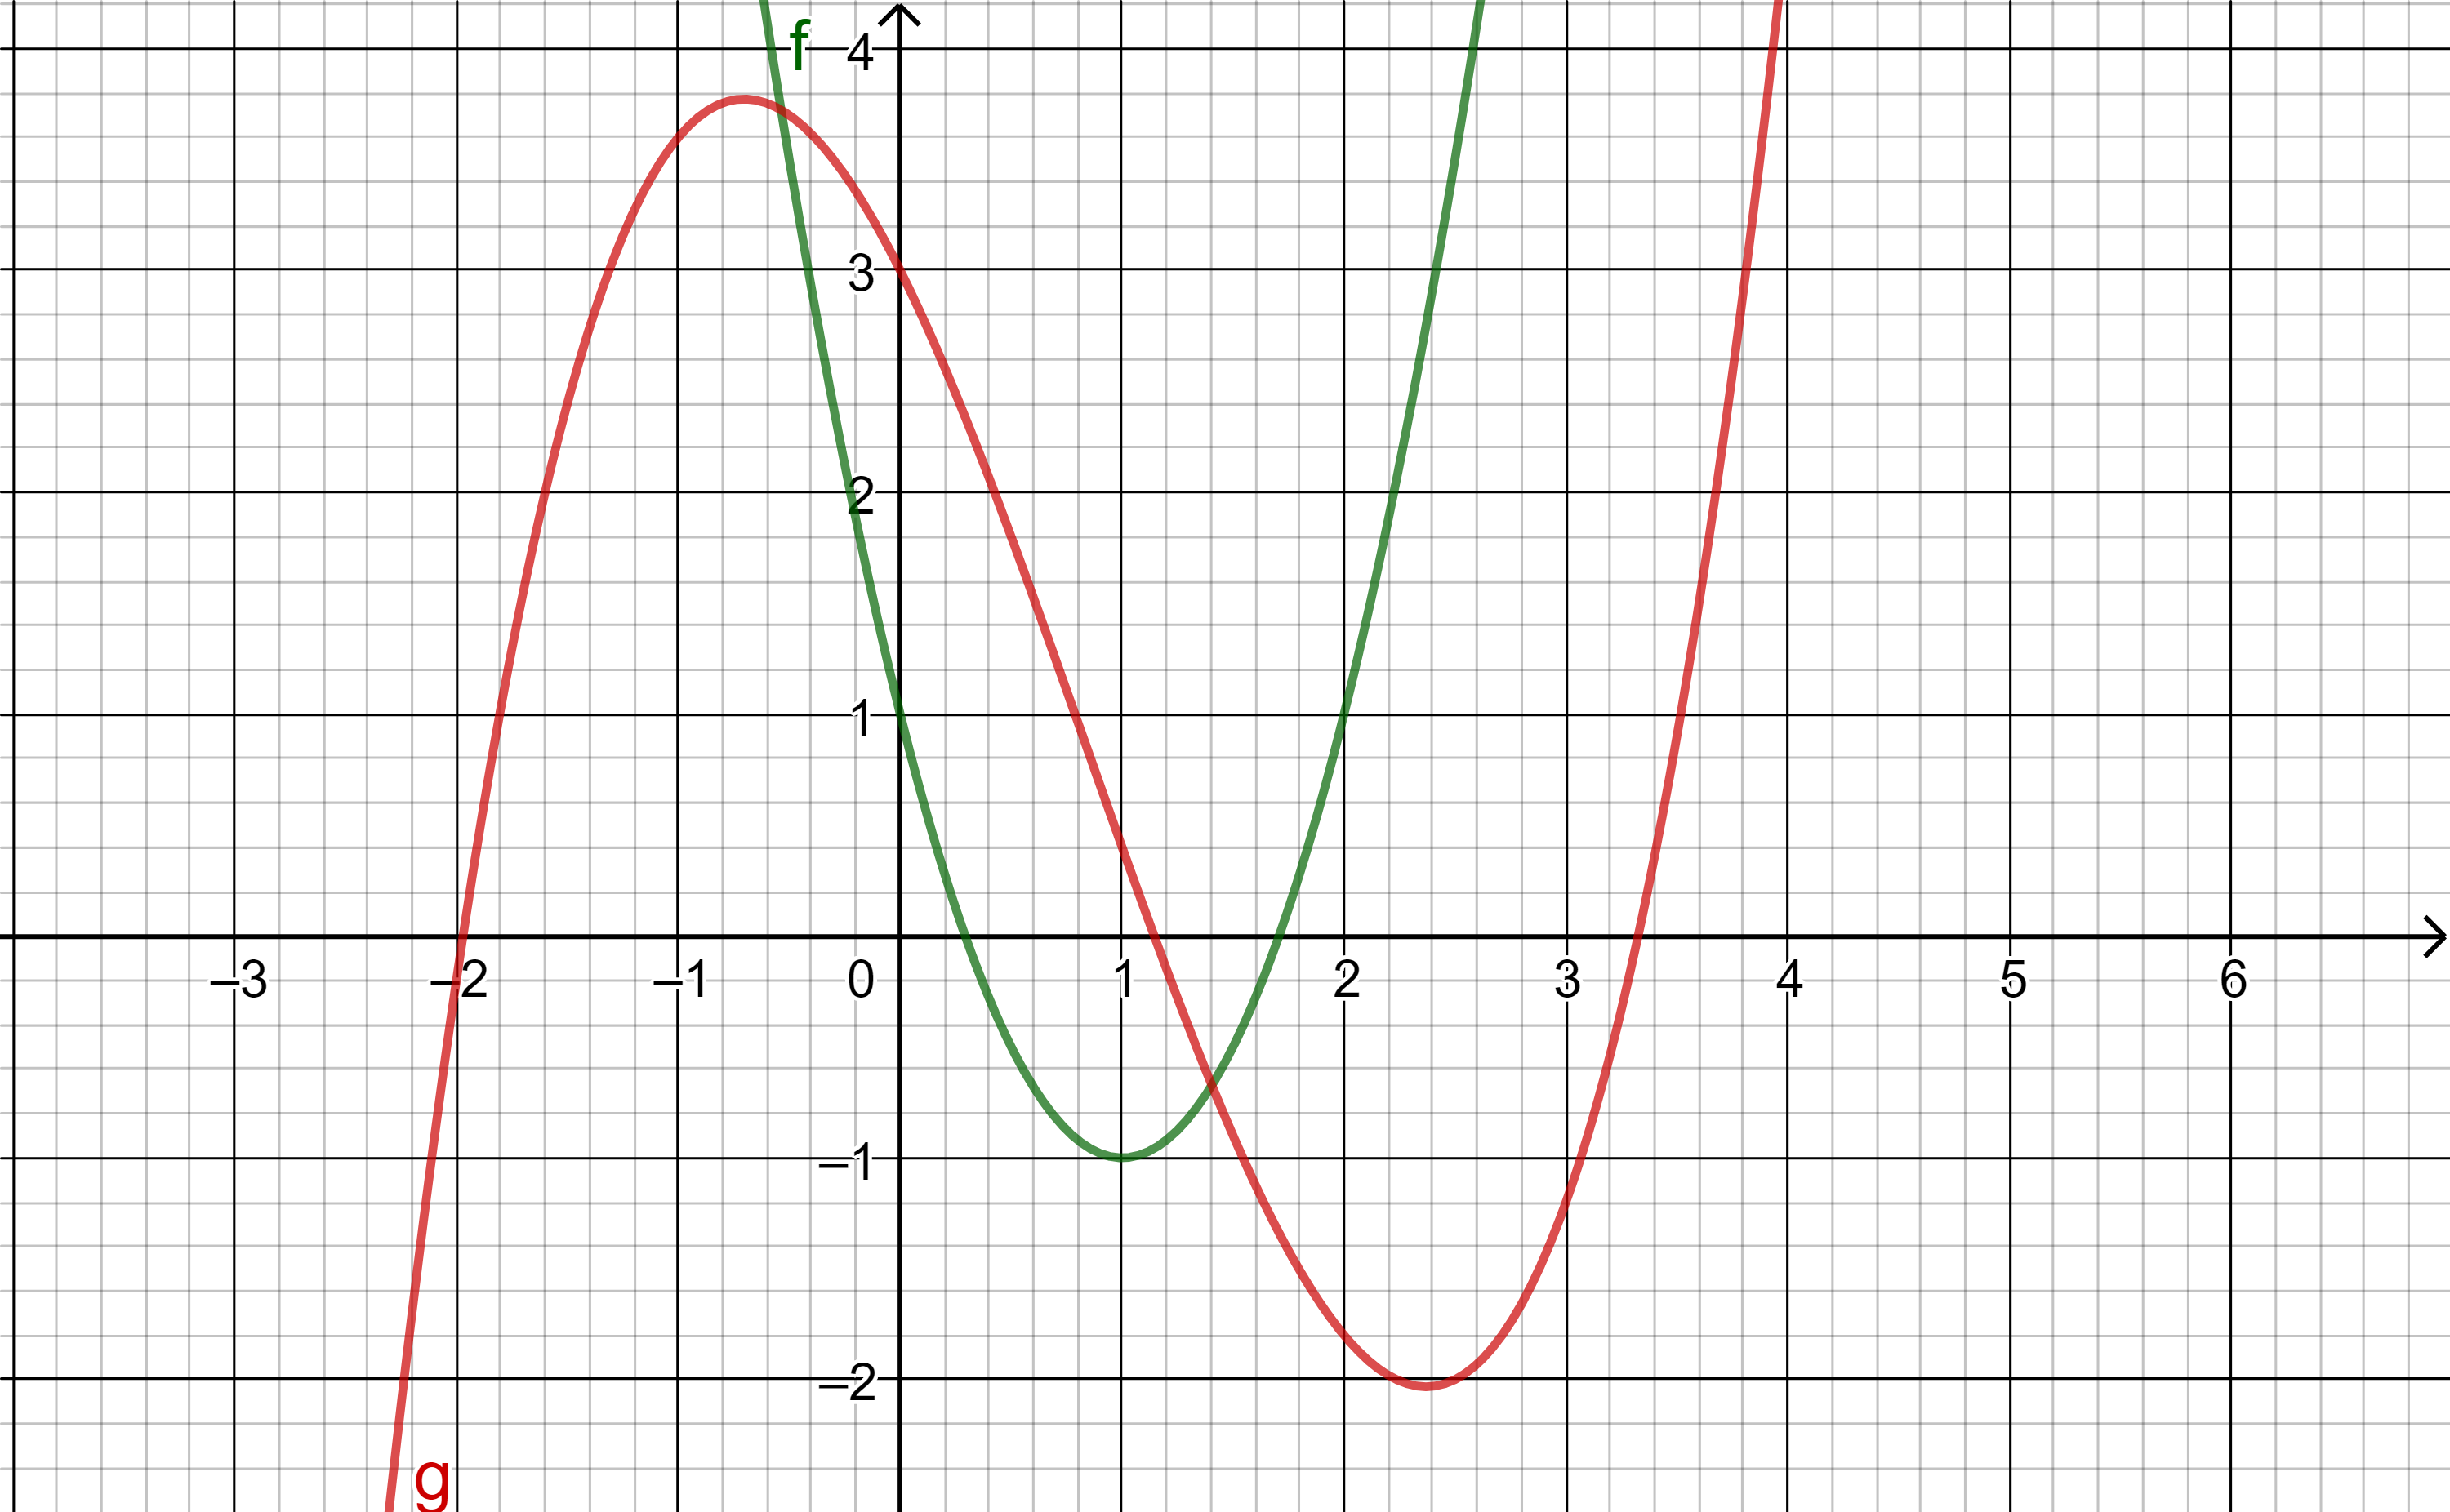
\includegraphics[width=0.5\textwidth]{pics/graphen}\\
 Bestimme die Stellen (ungefähr) bei denen der Funktionswert von f und der von g übereinstimmt.\\ }
    \solution{ }
    \end{Add}
    \begin{Add}{MaI}{basal1}{Funktionsauswertung}{leicht}
    \question{ Gegeben sind die Graphen der Funktionen f und g. \\
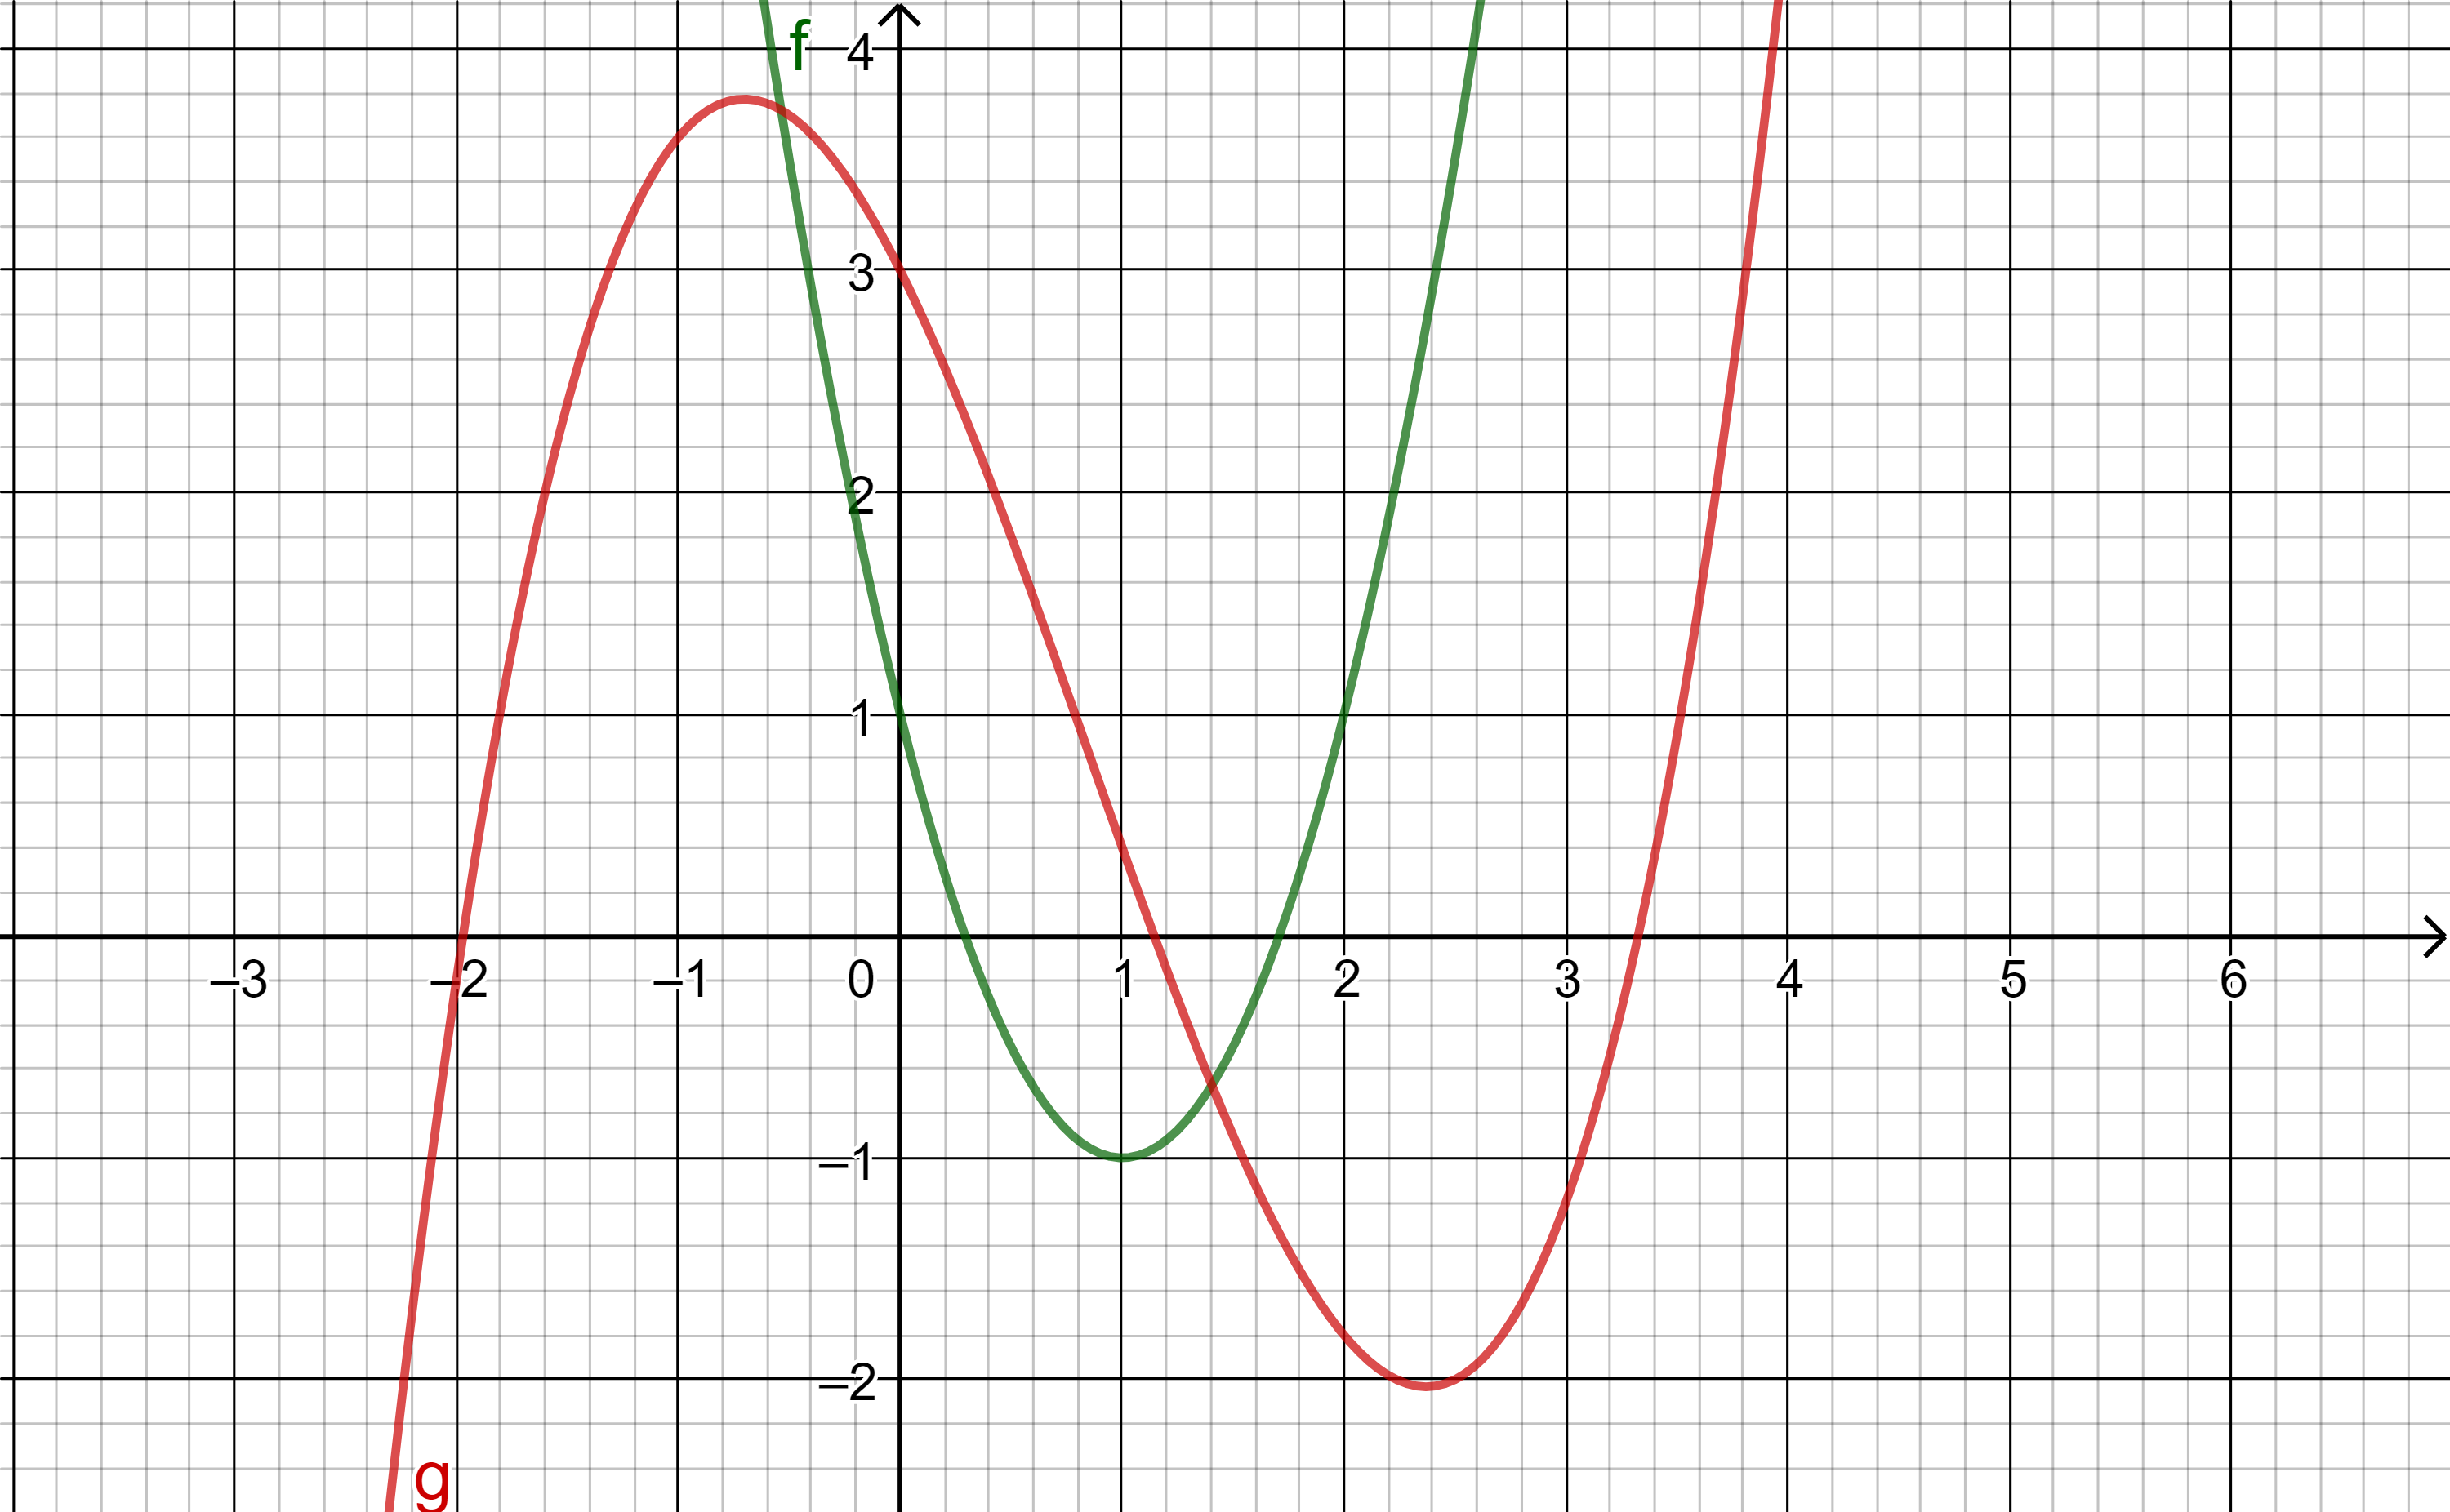
\includegraphics[width=0.5\textwidth]{pics/graphen}\\
 Bestimme die Stellen (ungefähr) bei denen der Funktionswert von f und der von g übereinstimmt.\\ }
    \solution{ $\frac{-1}{2}$ und $\frac{3}{2}$ }
    \end{Add}
    

    \begin{Add}{MaI}{basal1}{Funktionsauswertung}{leicht}
    \question{ Gegeben sind die Graphen der Funktionen f und g. \\
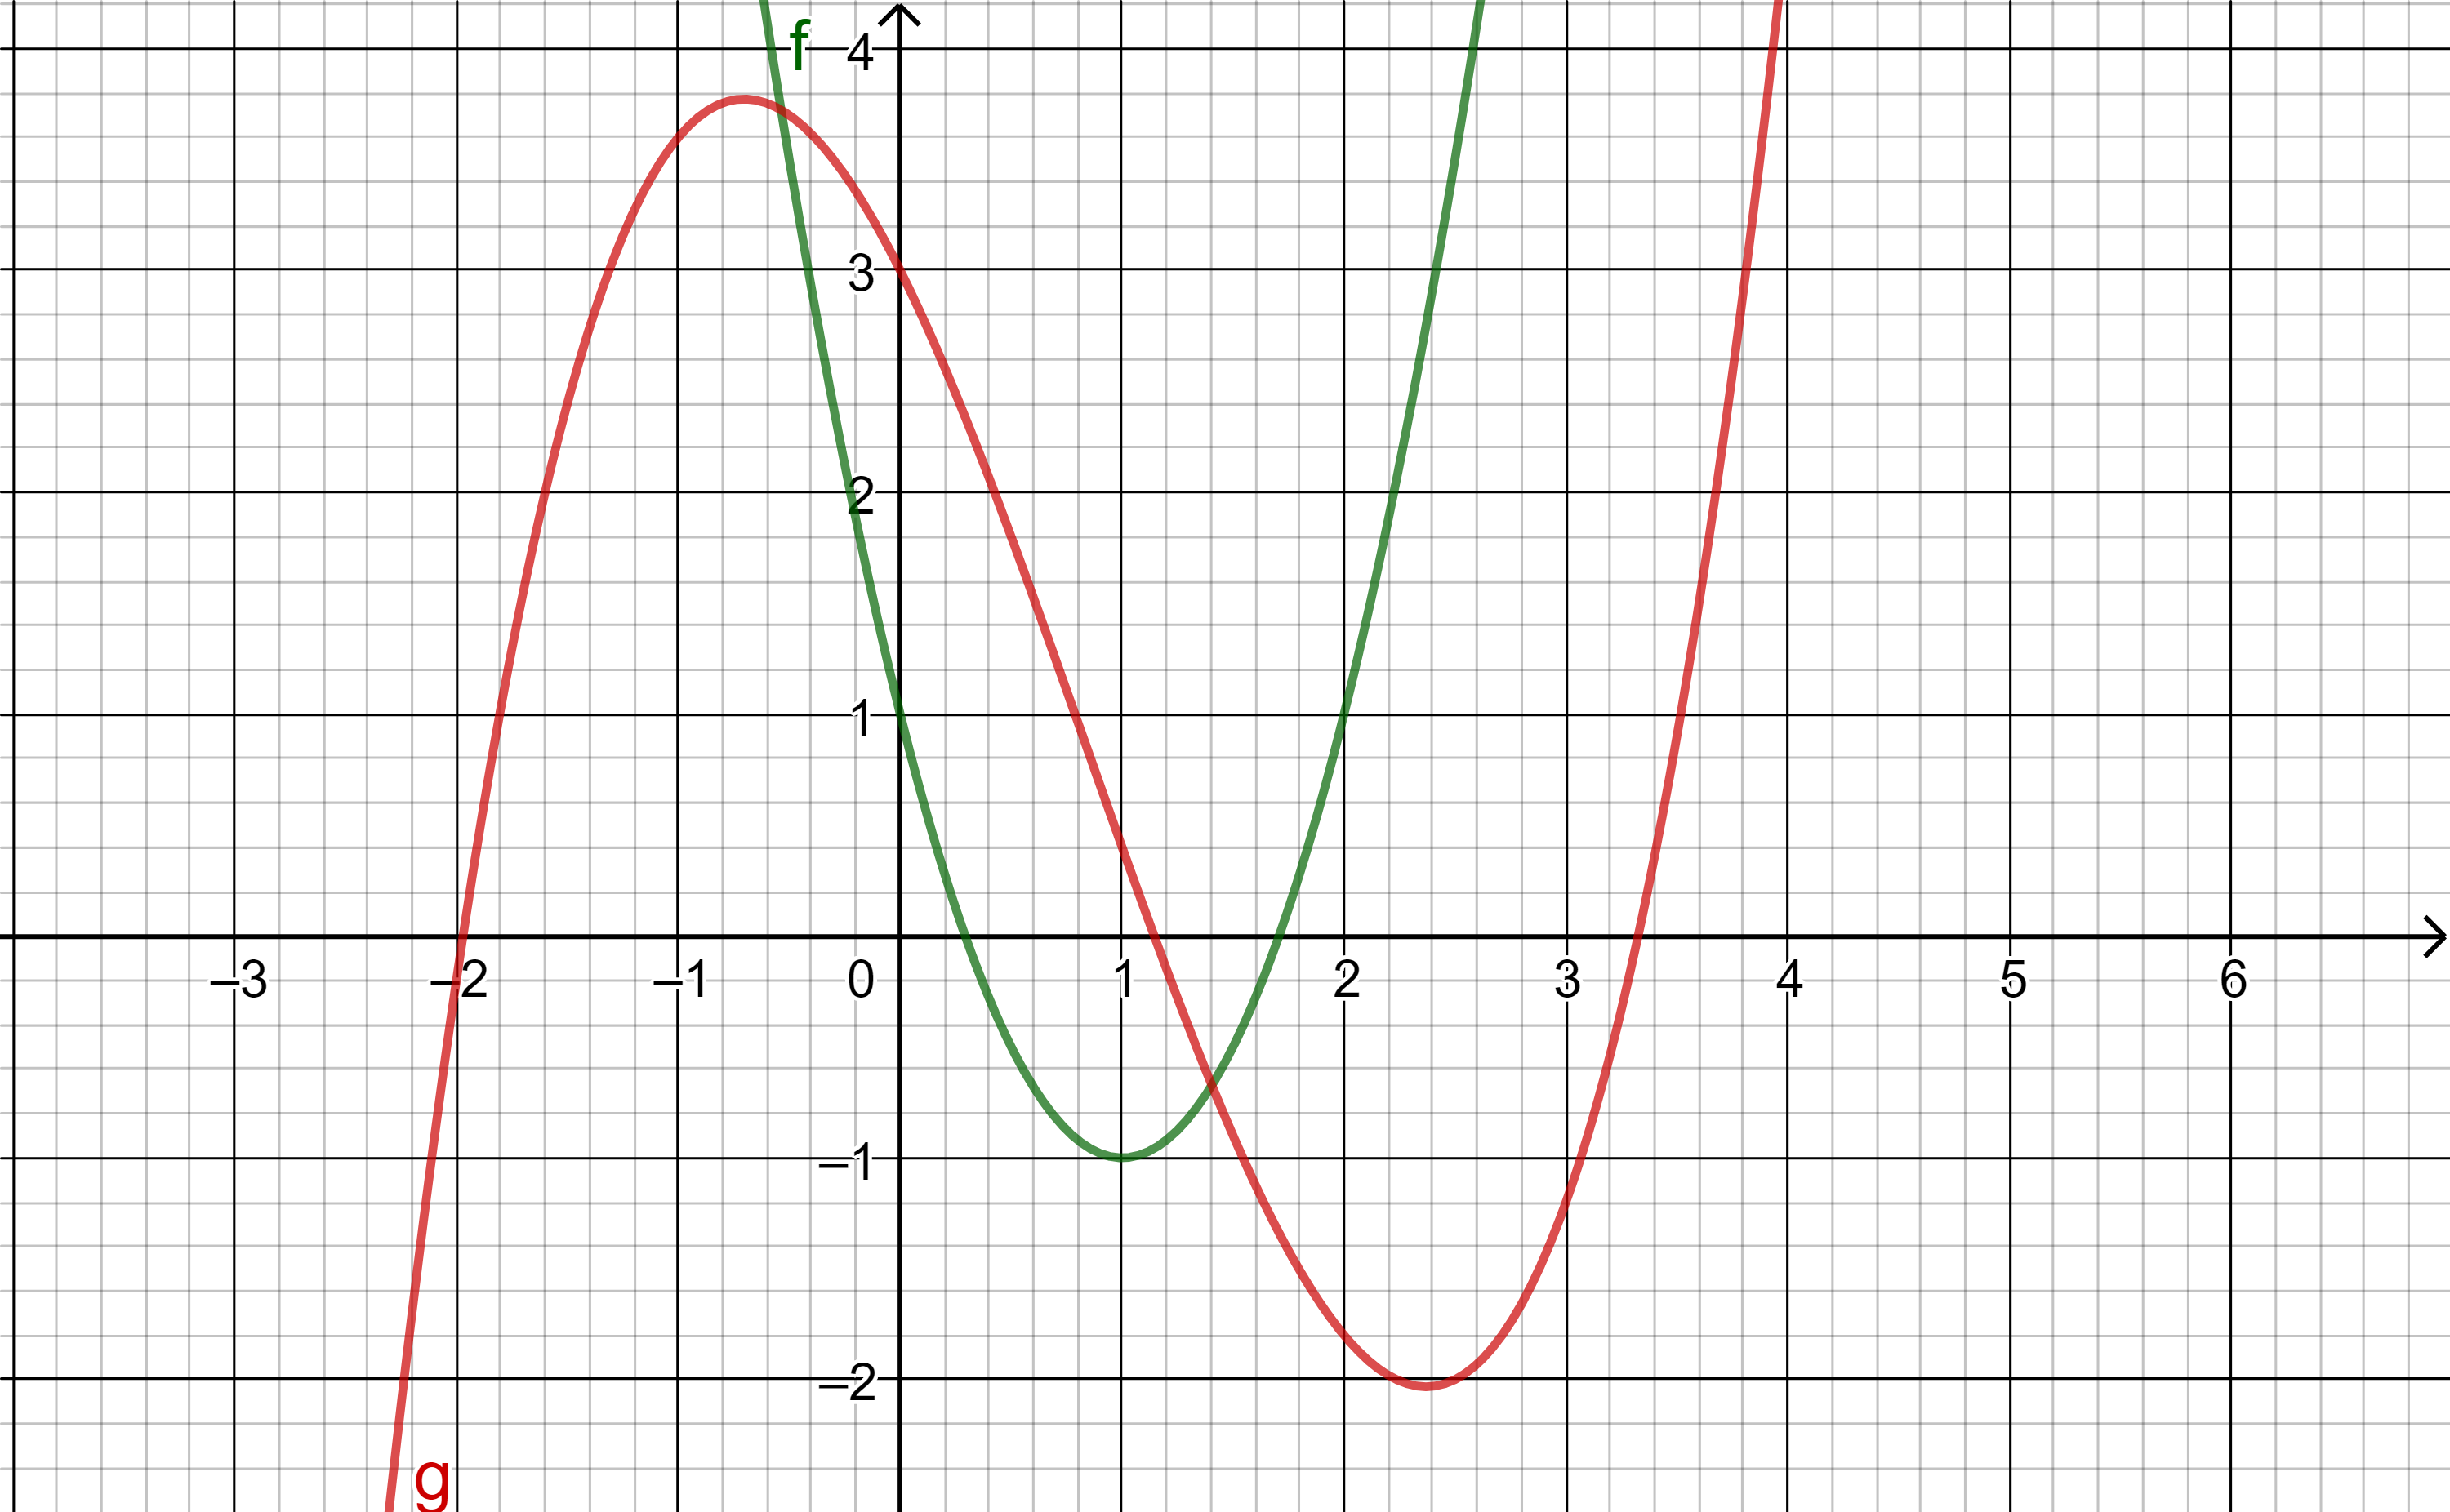
\includegraphics[width=0.5\textwidth]{pics/graphen}\\
Bestimme den Funktionswert von f an der Stelle Null.\\ }
    \solution{ }
    \end{Add}
    \begin{Add}{MaI}{basal1}{Funktionsauswertung}{leicht}
    \question{ Gegeben sind die Graphen der Funktionen f und g. \\
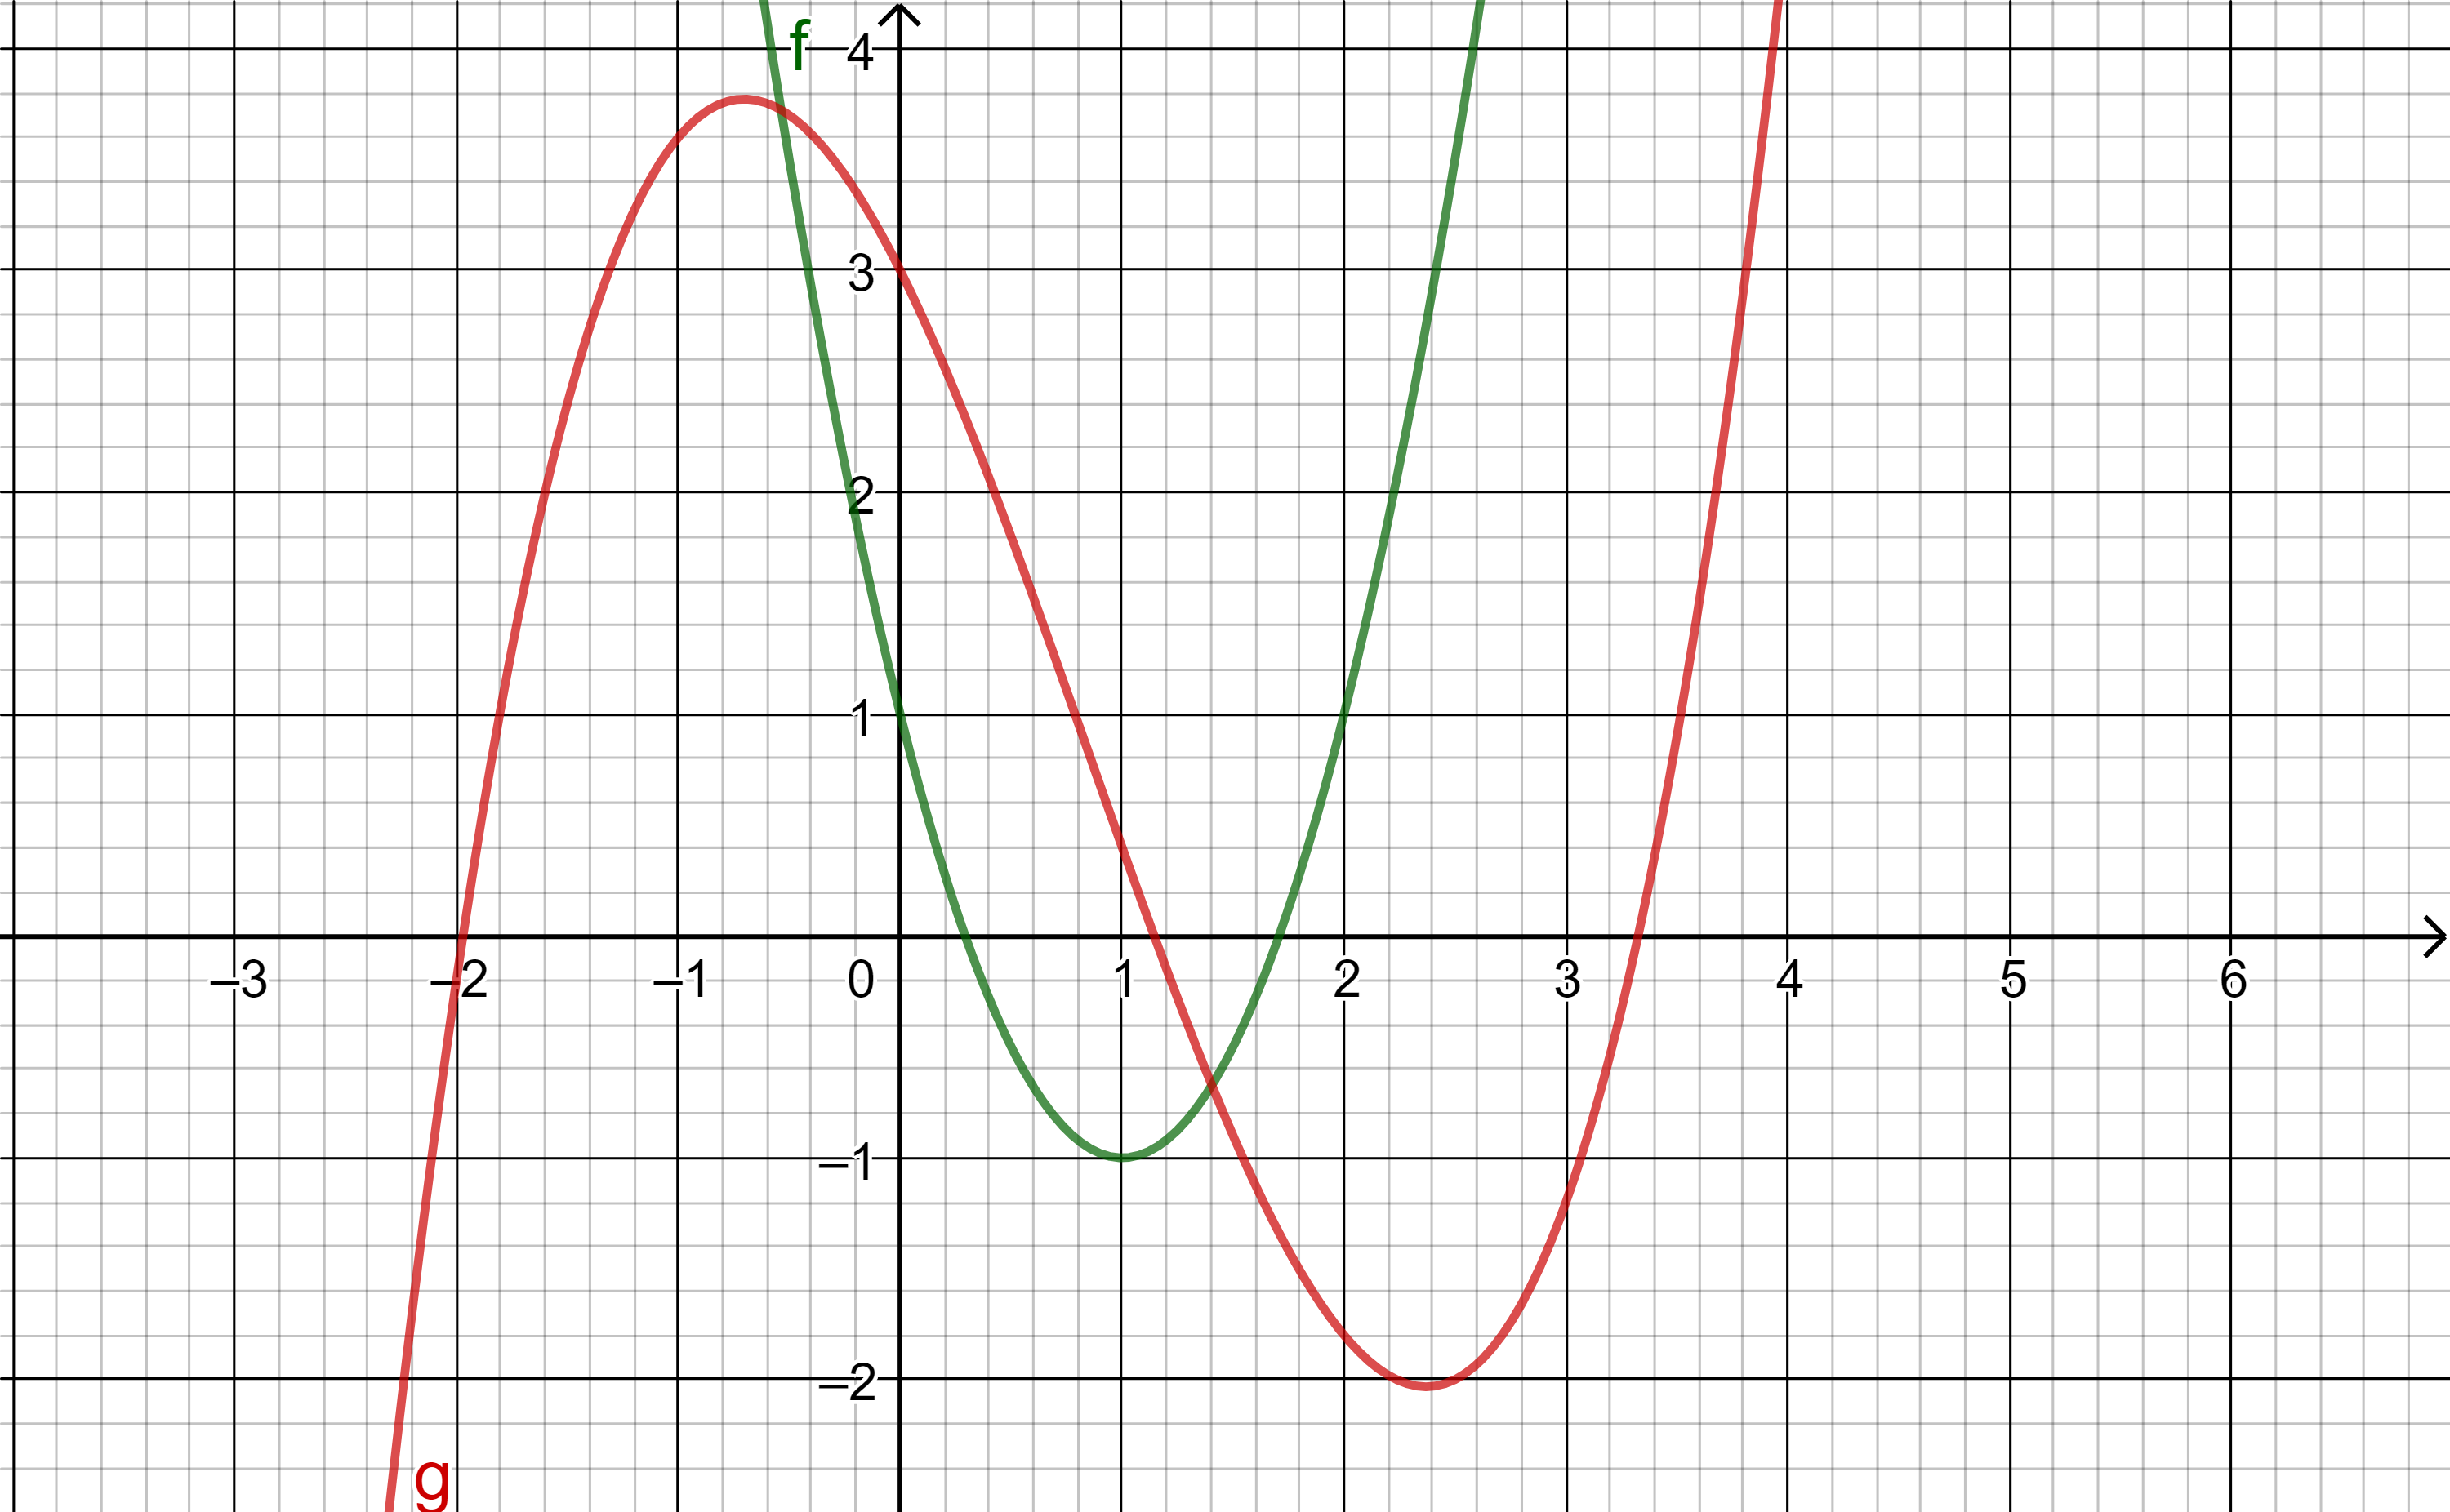
\includegraphics[width=0.5\textwidth]{pics/graphen}\\
Bestimme den Funktionswert von f an der Stelle Null.\\ }
    \solution{ $1$ }
    \end{Add}
    

    \begin{Add}{MaI}{basal1}{Funktionsauswertung}{leicht}
    \question{ Gegeben sind die Graphen der Funktionen f und g. \\
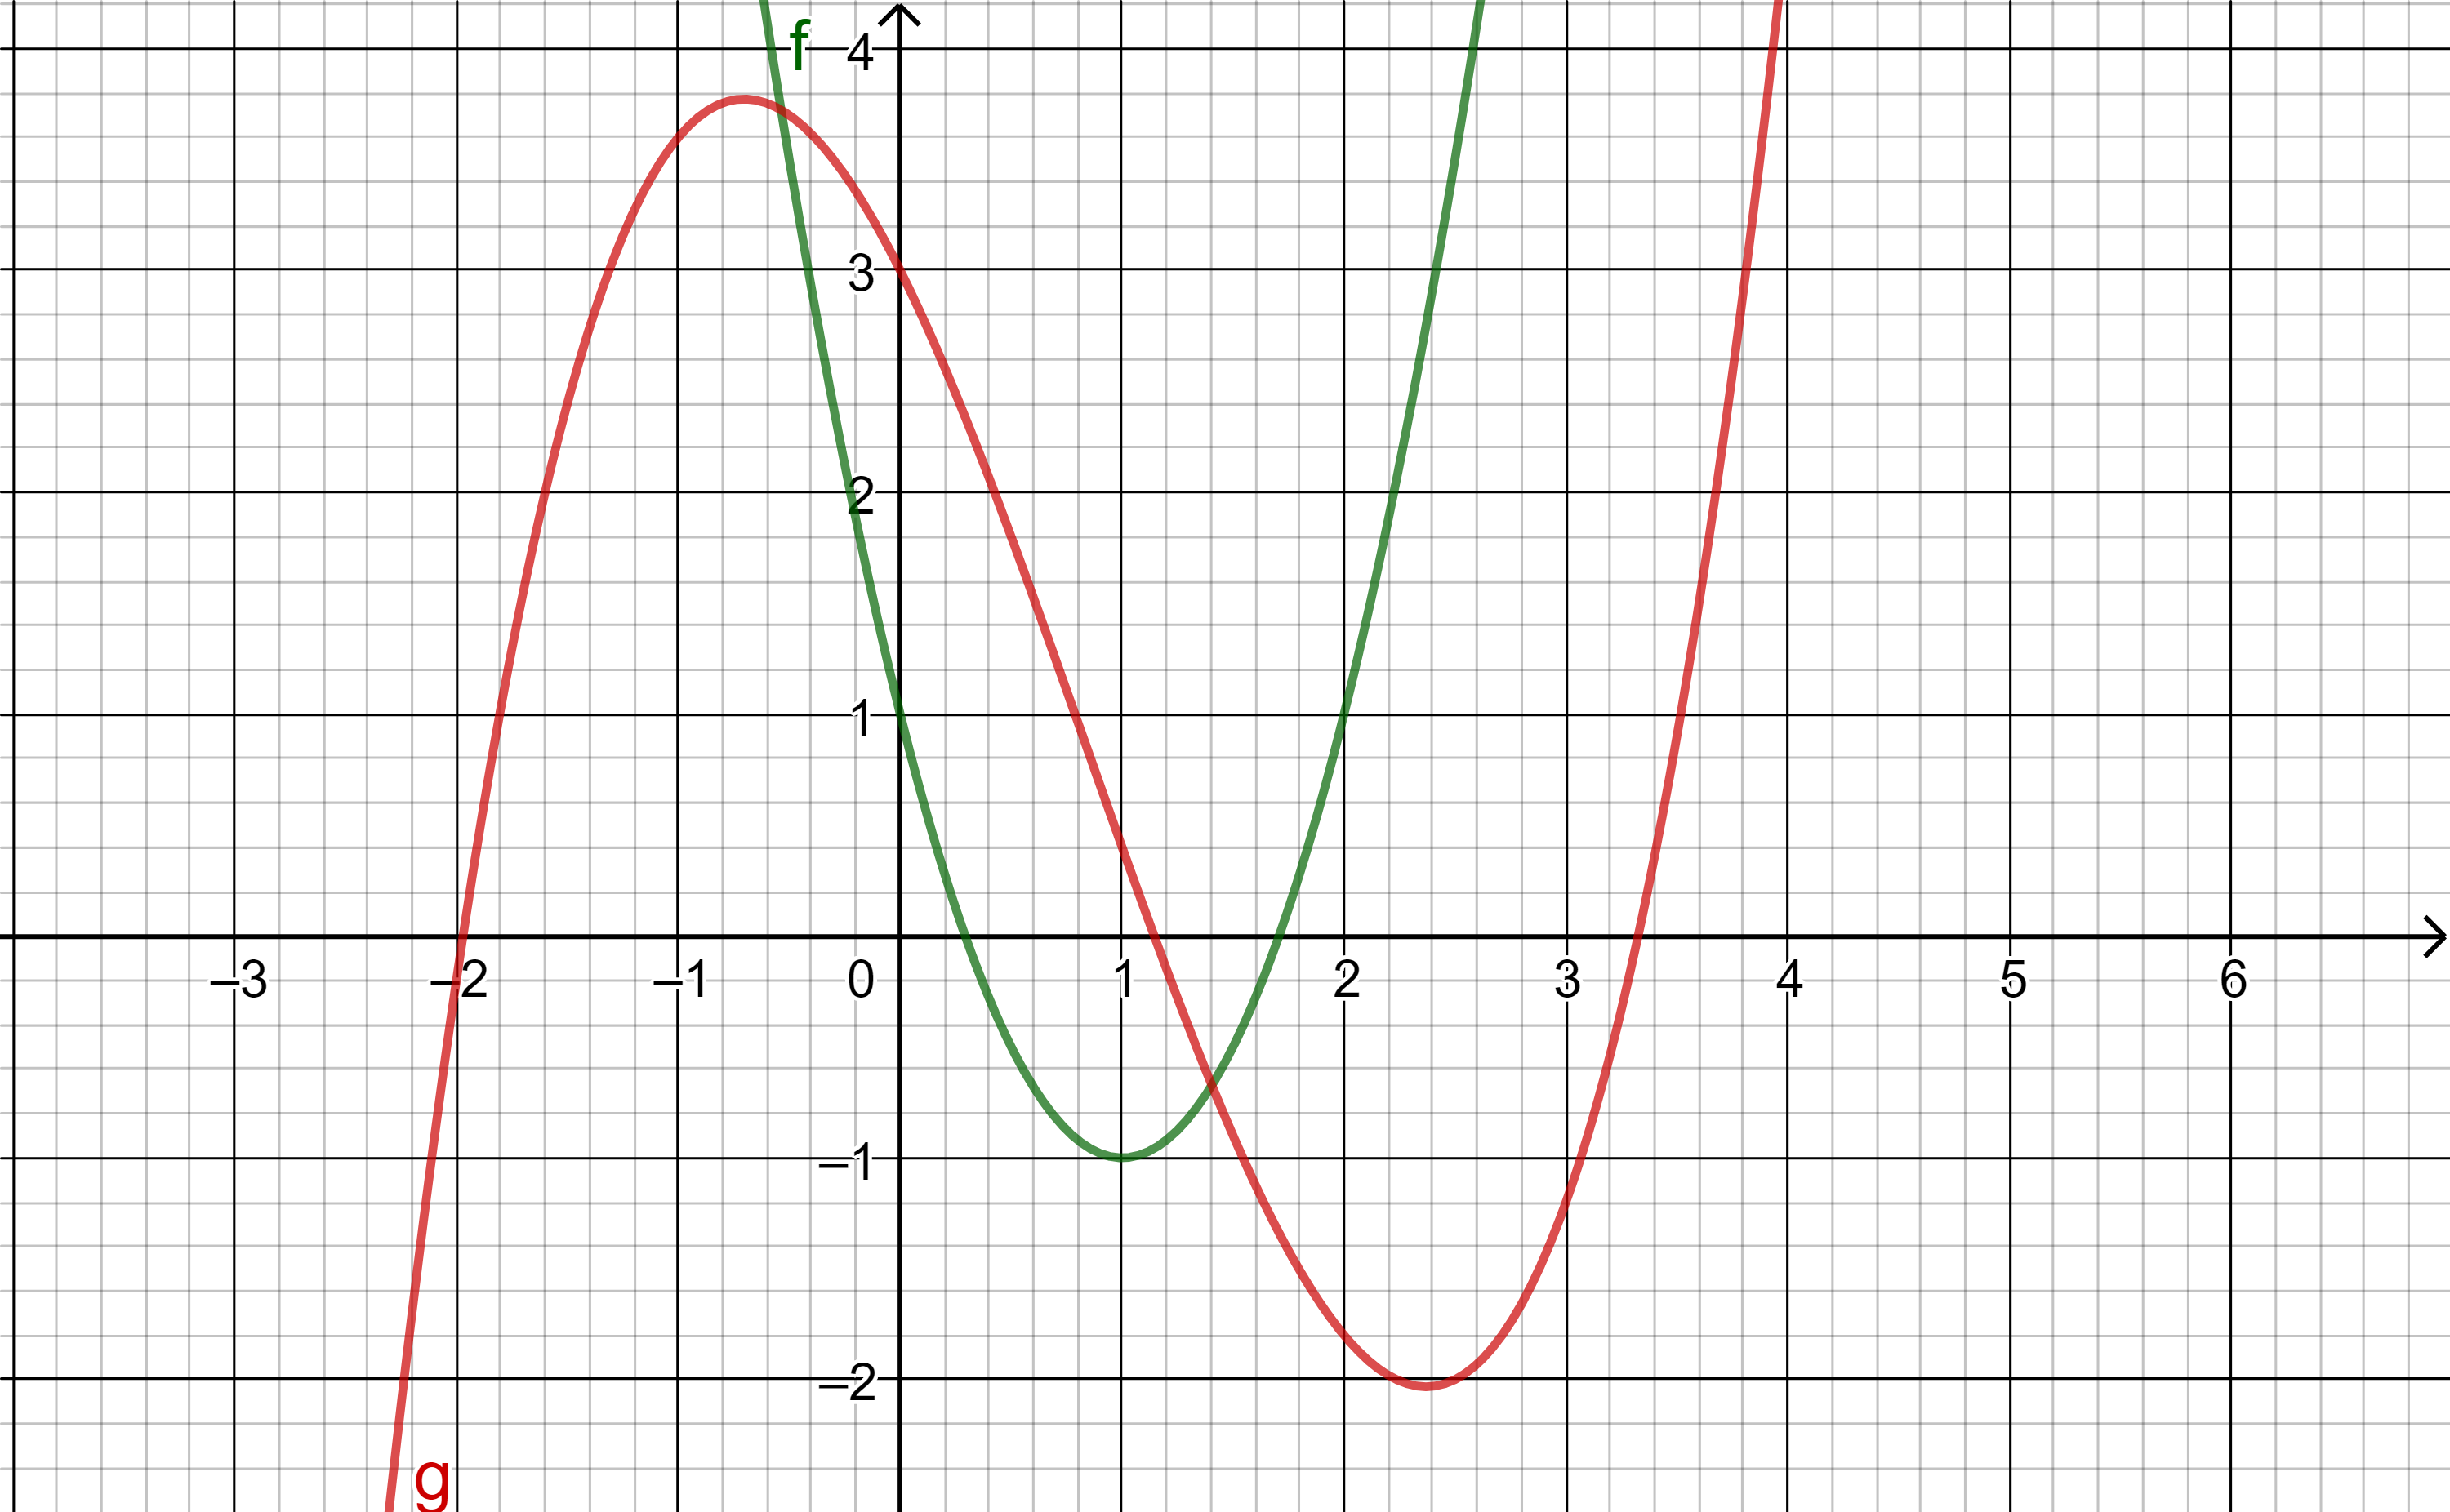
\includegraphics[width=0.5\textwidth]{pics/graphen}\\
An welcher Stelle ist der Funktionswert von f gleich $-1$.\\ }
    \solution{ }
    \end{Add}
    \begin{Add}{MaI}{basal1}{Funktionsauswertung}{leicht}
    \question{ Gegeben sind die Graphen der Funktionen f und g. \\
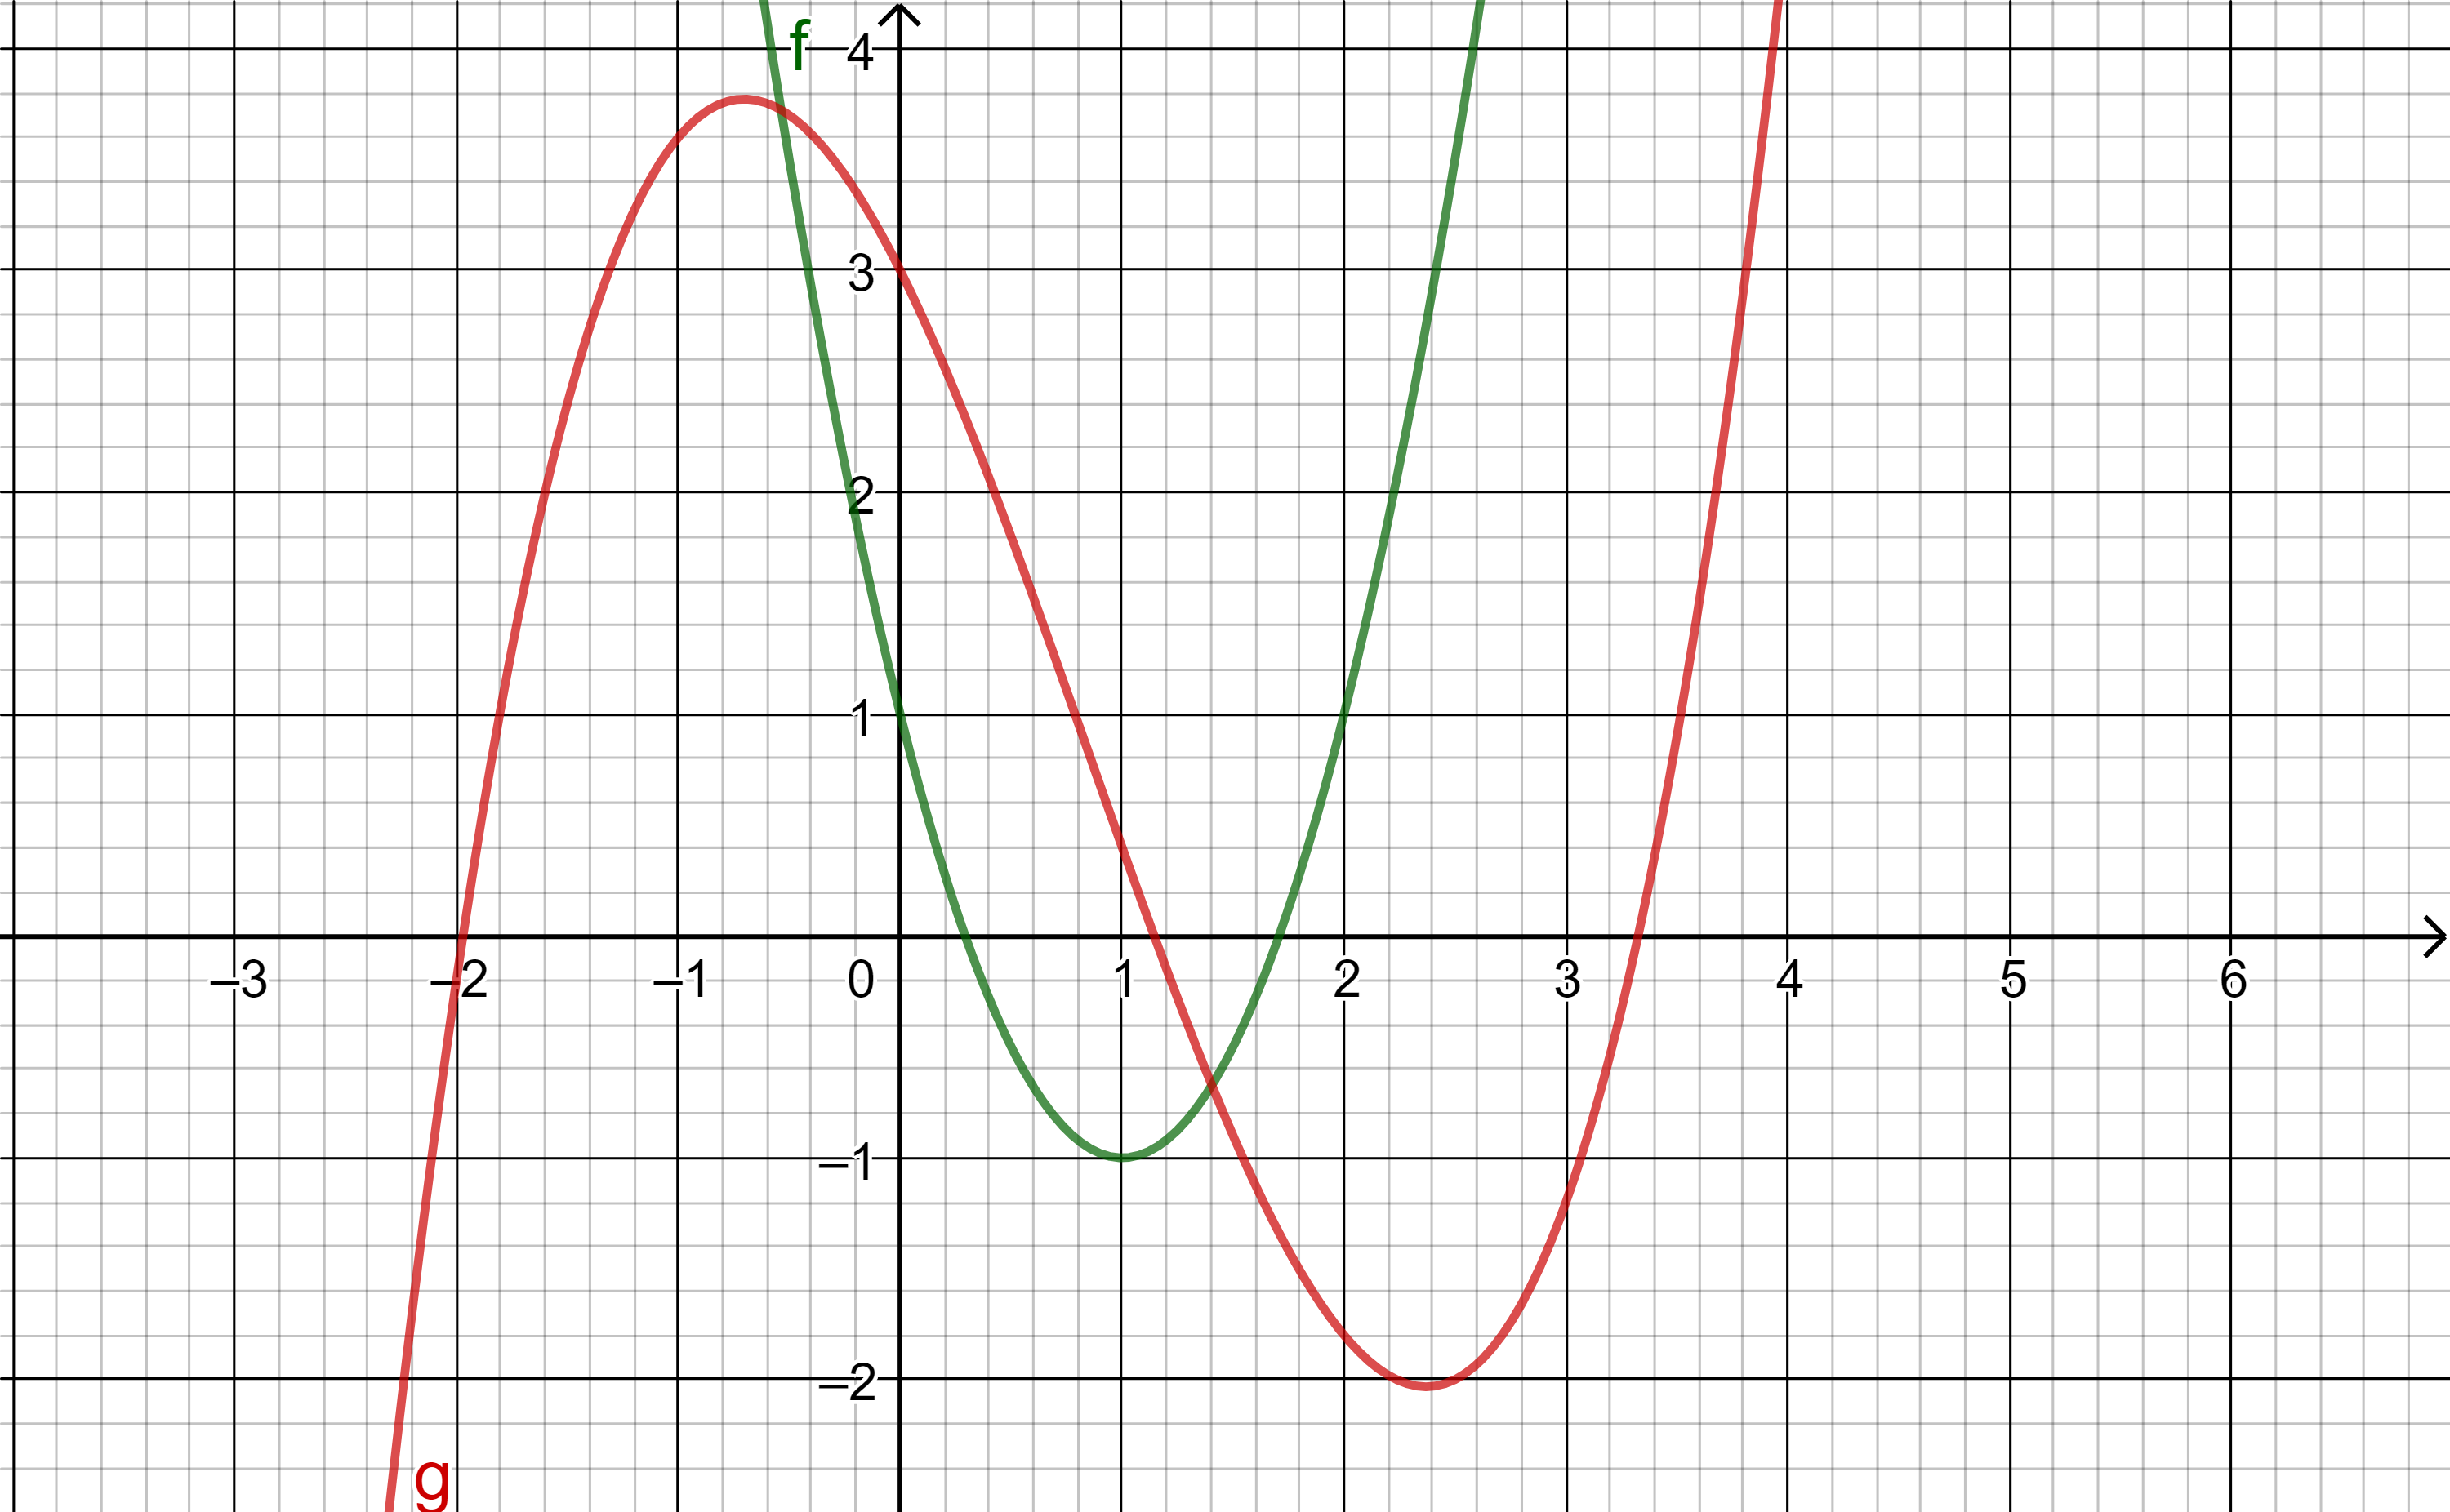
\includegraphics[width=0.5\textwidth]{pics/graphen}\\
An welcher Stelle ist der Funktionswert von f gleich $-1$.\\ }
    \solution{ $1$ }
    \end{Add}
    

    \begin{Add}{MaI}{basal1}{Funktionsauswertung}{leicht}
    \question{ Gegeben sind die Graphen der Funktionen f und g. \\
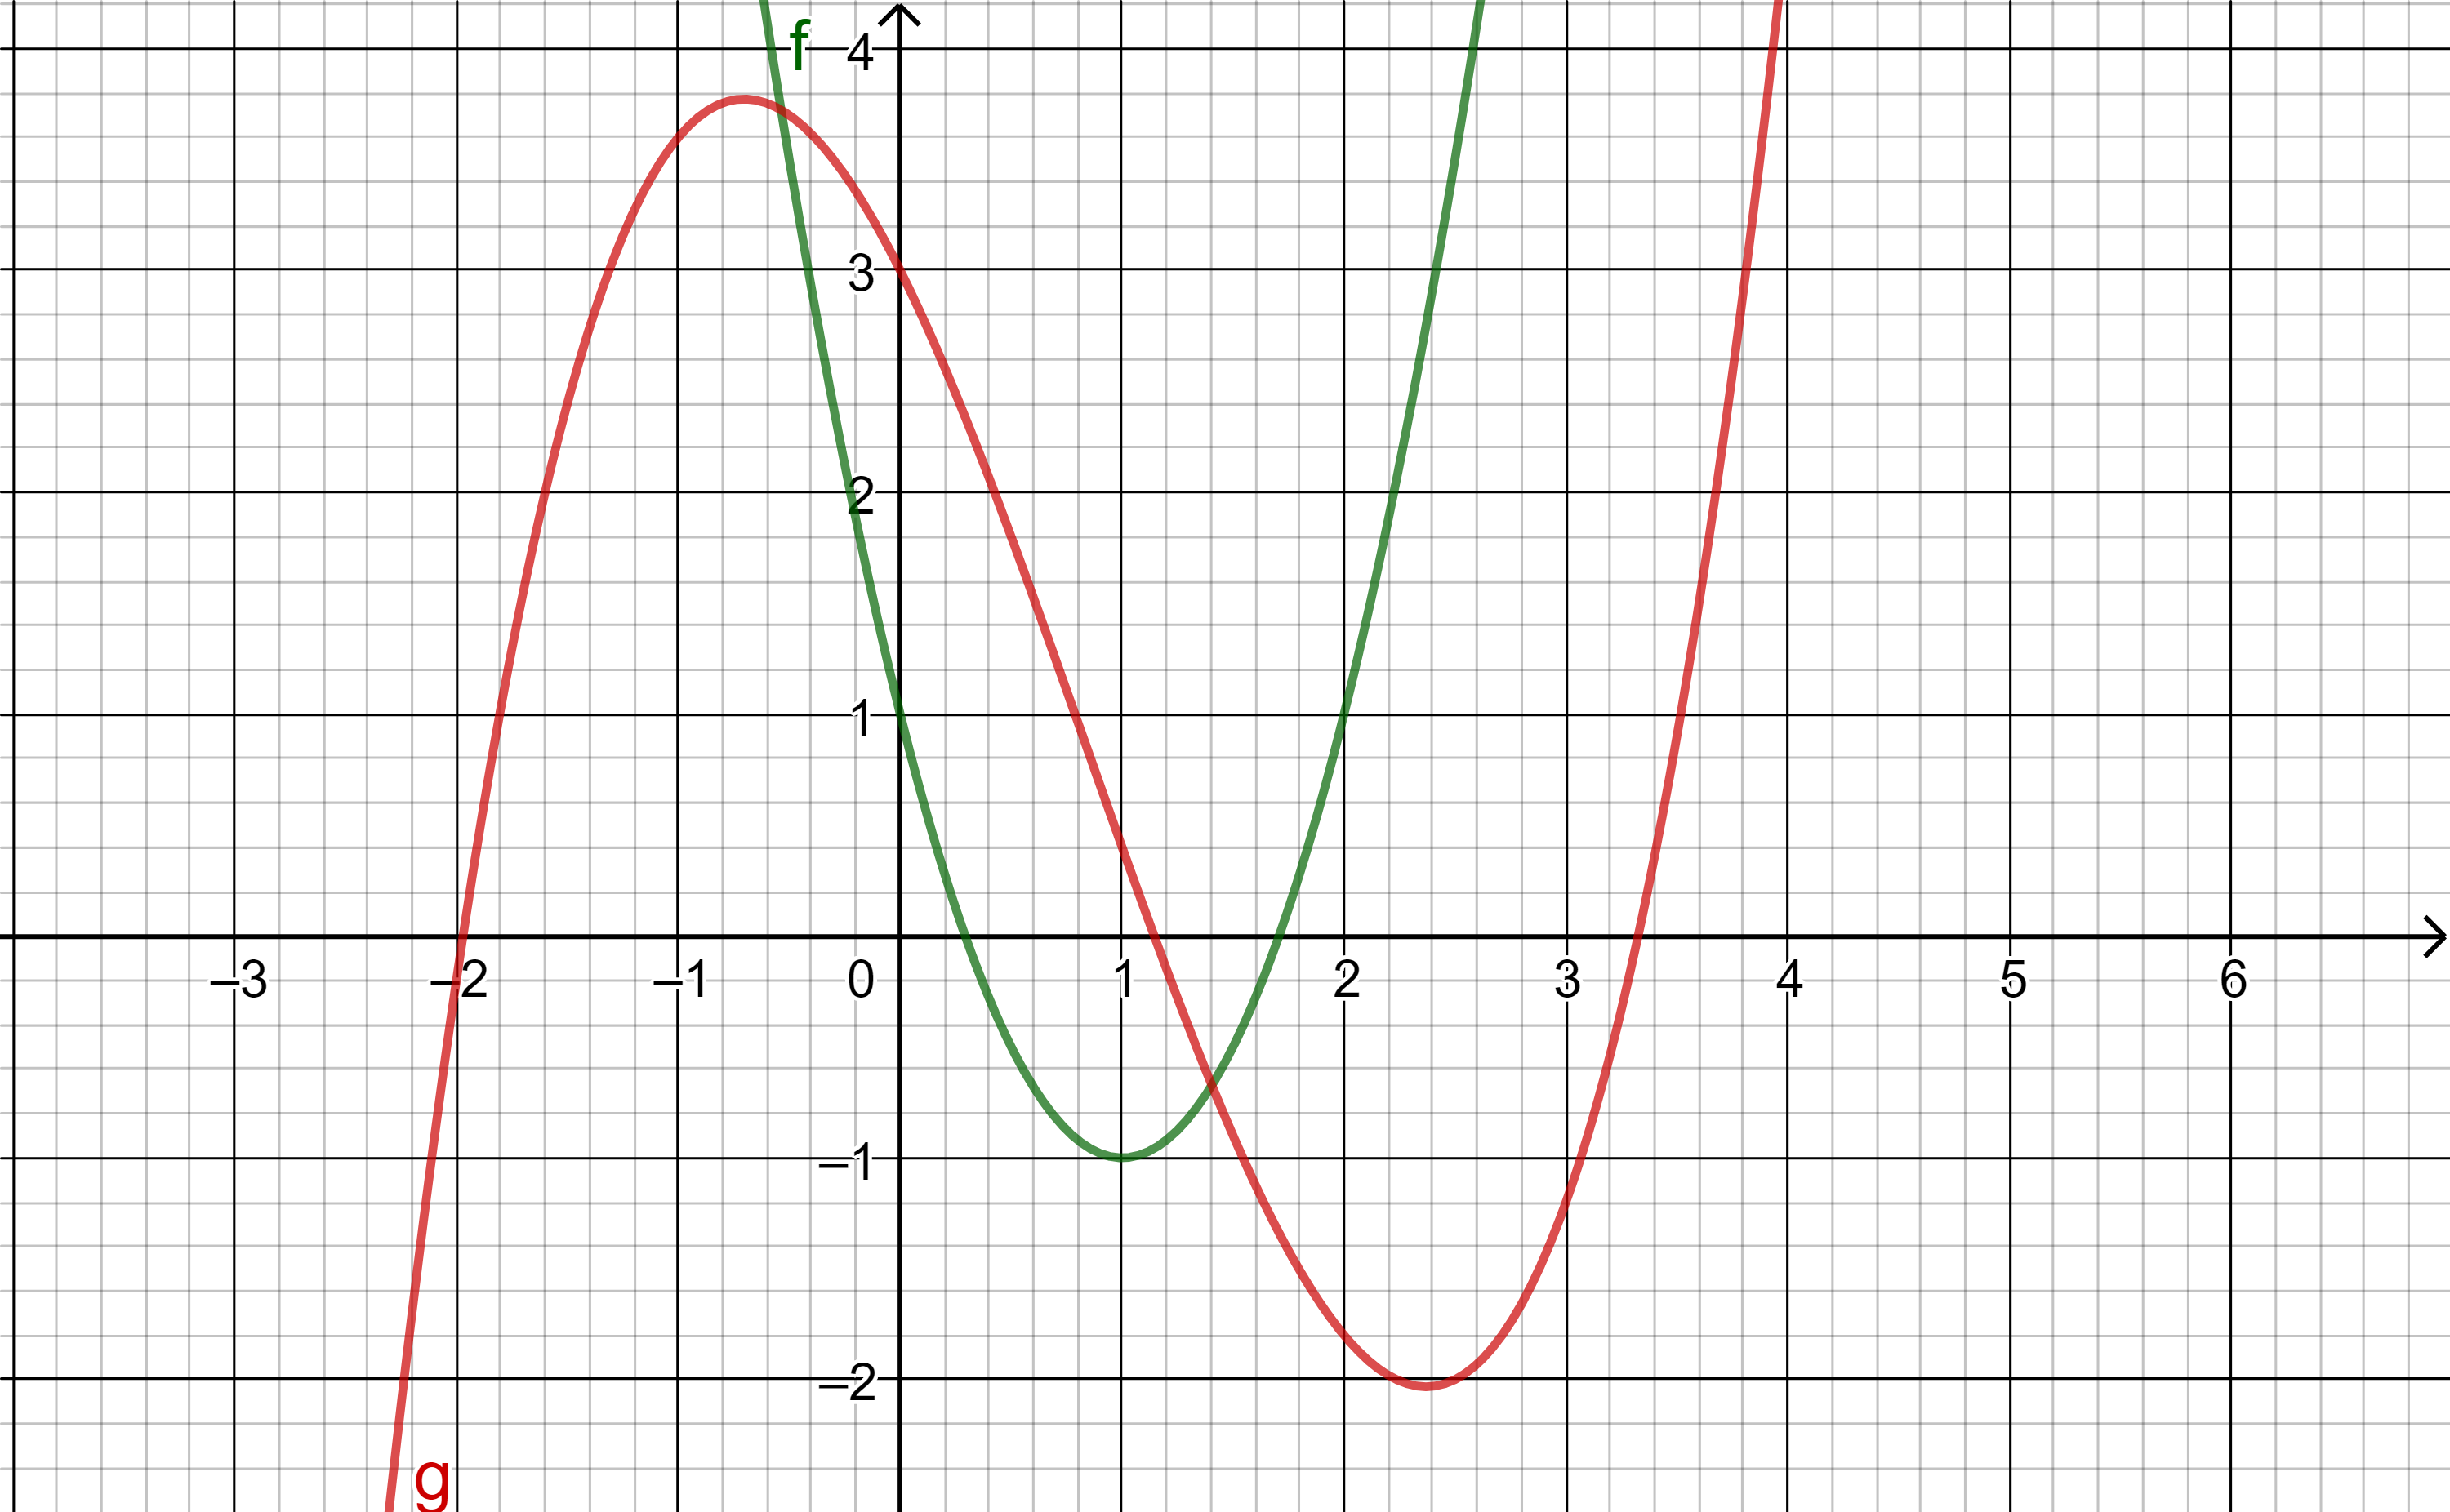
\includegraphics[width=0.5\textwidth]{pics/graphen}\\
Bestimme den Funktionswert von g an der Stelle Null.\\ }
    \solution{ }
    \end{Add}
    \begin{Add}{MaI}{basal1}{Funktionsauswertung}{leicht}
    \question{ Gegeben sind die Graphen der Funktionen f und g. \\
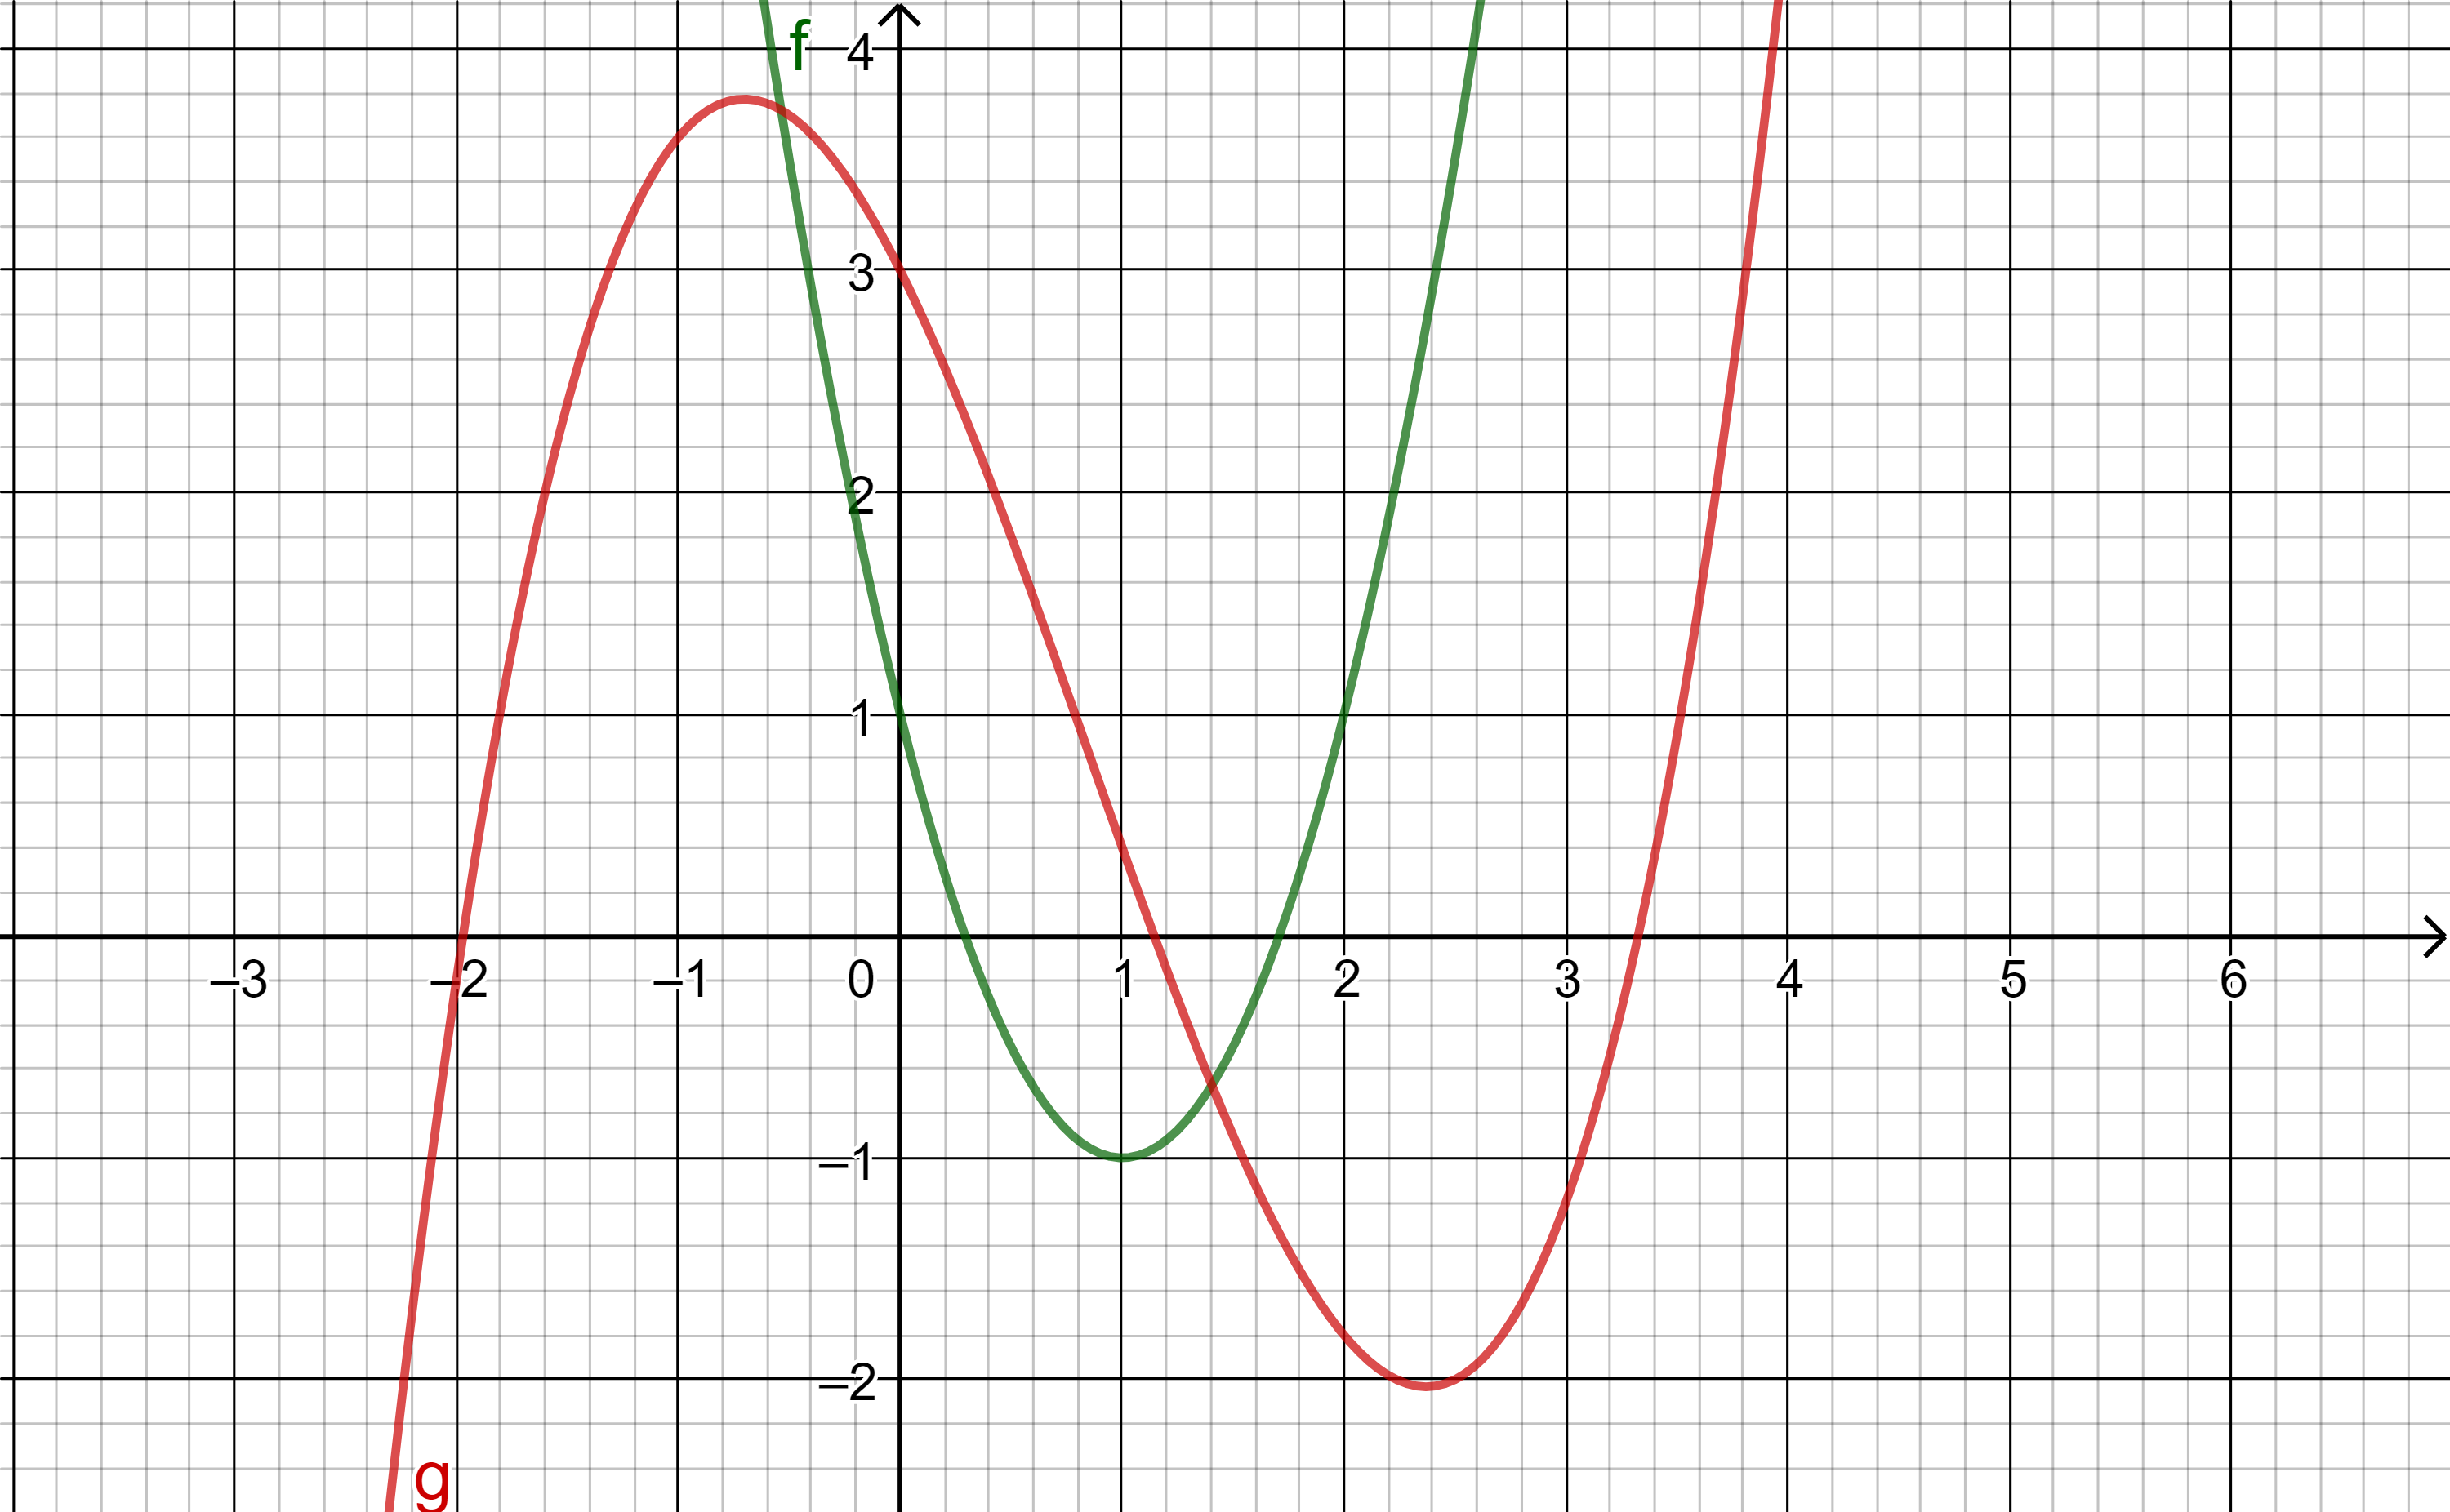
\includegraphics[width=0.5\textwidth]{pics/graphen}\\
Bestimme den Funktionswert von g an der Stelle Null.\\ }
    \solution{ $3$ }
    \end{Add}
    

    \begin{Add}{MaI}{basal1}{Wurzel}{leicht}
    \question{ Vereinfache:
$$\sqrt{a^2+b^2}=\;?$$
$$\sqrt{a^2 \cdot b^2}=\;?$$
$$\sqrt{\frac{a^2}{b^2}}=\;?$$ }
    \solution{ }
    \end{Add}
    \begin{Add}{MaI}{basal1}{Wurzel}{leicht}
    \question{ Vereinfache:
$$\sqrt{a^2+b^2}=\;?$$
$$\sqrt{a^2 \cdot b^2}=\;?$$
$$\sqrt{\frac{a^2}{b^2}}=\;?$$ }
    \solution{ $\sqrt{a^2+b^2}$ , $a \cdot b$ und $\frac{a}{b}$ }
    \end{Add}
    

    \begin{Add}{MaI}{basal1}{Wurzel, BinomischeFormeln}{mittel}
    \question{ Vereinfache:
$$\sqrt{4a^2+4a+1}=\;?$$ }
    \solution{ }
    \end{Add}
    \begin{Add}{MaI}{basal1}{Wurzel, BinomischeFormeln}{mittel}
    \question{ Vereinfache:
$$\sqrt{4a^2+4a+1}=\;?$$ }
    \solution{ $2a+1$ }
    \end{Add}
    

    \begin{Add}{MaI}{basal1}{Wurzel, BinomischeFormeln}{mittel}
    \question{ Vereinfache:
$$\sqrt{36x^2+24x+4}=\;?$$ }
    \solution{ }
    \end{Add}
    \begin{Add}{MaI}{basal1}{Wurzel, BinomischeFormeln}{mittel}
    \question{ Vereinfache:
$$\sqrt{36x^2+24x+4}=\;?$$ }
    \solution{ $2(3x+1)$ }
    \end{Add}
    

    \begin{Add}{MaI}{basal1}{Wurzel, BinomischeFormeln}{mittel}
    \question{ Vereinfache:
$$\sqrt{4a^2x^2-36a^2}=\;?$$ }
    \solution{ }
    \end{Add}
    \begin{Add}{MaI}{basal1}{Wurzel, BinomischeFormeln}{mittel}
    \question{ Vereinfache:
$$\sqrt{4a^2x^2-36a^2}=\;?$$ }
    \solution{ $2a\sqrt{(x+3)(x-3)}$ }
    \end{Add}
    

    \begin{Add}{MaI}{basal1}{Wurzel, BinomischeFormeln}{mittel}
    \question{ Vereinfache:
$$\sqrt{a^4-4a^3b+4a^2b^2}=\;?$$ }
    \solution{ }
    \end{Add}
    \begin{Add}{MaI}{basal1}{Wurzel, BinomischeFormeln}{mittel}
    \question{ Vereinfache:
$$\sqrt{a^4-4a^3b+4a^2b^2}=\;?$$ }
    \solution{ $a(a-2b)$ }
    \end{Add}
    

    \begin{Add}{MaI}{basal1}{Termumformungen}{leicht}
    \question{ Faktorisiere:
$$x^4y^2-x^2y^4$$ }
    \solution{ }
    \end{Add}
    \begin{Add}{MaI}{basal1}{Termumformungen}{leicht}
    \question{ Faktorisiere:
$$x^4y^2-x^2y^4$$ }
    \solution{ $x^2y^2(x^2-y^2)$ }
    \end{Add}
    

    \begin{Add}{MaI}{basal1}{Termumformungen}{leicht}
    \question{ Faktorisiere:
$$3x^2y^2-3x^2z^2$$ }
    \solution{ }
    \end{Add}
    \begin{Add}{MaI}{basal1}{Termumformungen}{leicht}
    \question{ Faktorisiere:
$$3x^2y^2-3x^2z^2$$ }
    \solution{ $3x^2(y-z)(y+z)$ }
    \end{Add}
    

    \begin{Add}{MaI}{basal1}{Termumformungen}{leicht}
    \question{ Fasse zusammen:
$$\frac{3z}{x^2y}+\frac{z^2}{xy^3}+\frac{2z^3}{x^3y^2}$$ }
    \solution{ }
    \end{Add}
    \begin{Add}{MaI}{basal1}{Termumformungen}{leicht}
    \question{ Fasse zusammen:
$$\frac{3z}{x^2y}+\frac{z^2}{xy^3}+\frac{2z^3}{x^3y^2}$$ }
    \solution{ $\frac{3xy^2z+x^2z^2+2yz^3}{x^3y^3}$ }
    \end{Add}
    

    \begin{Add}{MaI}{basal1}{Termumformungen}{leicht}
    \question{ Vereinfache:
$$\frac{p^7}{r}\left(\frac{q^5}{p^4}\div\frac{q^8}{r^4}\right)$$ }
    \solution{ }
    \end{Add}
    \begin{Add}{MaI}{basal1}{Termumformungen}{leicht}
    \question{ Vereinfache:
$$\frac{p^7}{r}\left(\frac{q^5}{p^4}\div\frac{q^8}{r^4}\right)$$ }
    \solution{ $\frac{p^3r^3}{q^3}$ }
    \end{Add}
    

   \begin{Add}{MaI}{basal1}{Termumformungen}{leicht}
   \question{ Fasse zusammen:
$$\frac{2a}{3a-3b}+\frac{a-b}{a-b}+\frac{b}{3a}$$ }
   \solution{ }
   \end{Add}
   \begin{Add}{MaI}{basal1}{Termumformungen}{leicht}
   \question{ Fasse zusammen:
$$\frac{2a}{3a-3b}+\frac{a-b}{a-b}+\frac{b}{3a}$$ }
   \solution{ $\frac{5a^2-2ab-b^2}{3a(a-b)}$ }
   \end{Add}
   

   \begin{Add}{MaI}{basal1}{Termumformungen}{leicht}
   \question{ Fasse zusammen:
$$2+\frac{3z^2}{z^2-yz}-\frac{y}{z-y}$$ }
   \solution{ }
   \end{Add}
   \begin{Add}{MaI}{basal1}{Termumformungen}{leicht}
   \question{ Fasse zusammen:
$$2+\frac{3z^2}{z^2-yz}-\frac{y}{z-y}$$ }
   \solution{ $\frac{5z-3y}{z-y}$ }
   \end{Add}
   

   \begin{Add}{MaI}{basal1}{Termumformungen}{leicht}
   \question{ Berechne:
$$\frac{a^2}{bc}\div\left(1-\frac{a}{c}\right)$$ }
   \solution{ }
   \end{Add}
   \begin{Add}{MaI}{basal1}{Termumformungen}{leicht}
   \question{ Berechne:
$$\frac{a^2}{bc}\div\left(1-\frac{a}{c}\right)$$ }
   \solution{ $\frac{a^2}{b(c-a)}$ }
   \end{Add}
   

   \begin{Add}{MaI}{basal1}{Termumformungen}{leicht}
   \question{ Berechne:
$$\left(1-\frac{b}{a}\right)\cdot\frac{ab}{a-b}$$ }
   \solution{ }
   \end{Add}
   \begin{Add}{MaI}{basal1}{Termumformungen}{leicht}
   \question{ Berechne:
$$\left(1-\frac{b}{a}\right)\cdot\frac{ab}{a-b}$$ }
   \solution{ $b$ }
   \end{Add}
   

   \begin{Add}{MaI}{basal1}{Termumformungen}{leicht}
   \question{ Berechne:
$$\frac{5}{xy}\div\left(\frac{1}{y}-\frac{1}{x}\right)$$ }
   \solution{ }
   \end{Add}
   \begin{Add}{MaI}{basal1}{Termumformungen}{leicht}
   \question{ Berechne:
$$\frac{5}{xy}\div\left(\frac{1}{y}-\frac{1}{x}\right)$$ }
   \solution{ $\frac{5}{x-y}$ }
   \end{Add}
   

   \begin{Add}{MaI}{basal1}{Termumformungen}{leicht}
   \question{ Berechne:
$$\left(1+\frac{b-a}{a}\right)\cdot\left(1-\frac{b}{b-a}\right)$$ }
   \solution{ }
   \end{Add}
   \begin{Add}{MaI}{basal1}{Termumformungen}{leicht}
   \question{ Berechne:
$$\left(1+\frac{b-a}{a}\right)\cdot\left(1-\frac{b}{b-a}\right)$$ }
   \solution{ $\frac{b}{a-b}$ }
   \end{Add}
   

    \begin{Add}{MaI}{basal1}{LineareFunktionen}{leicht}
    \question{ Gegeben ist der Graph der Funktion f. \\
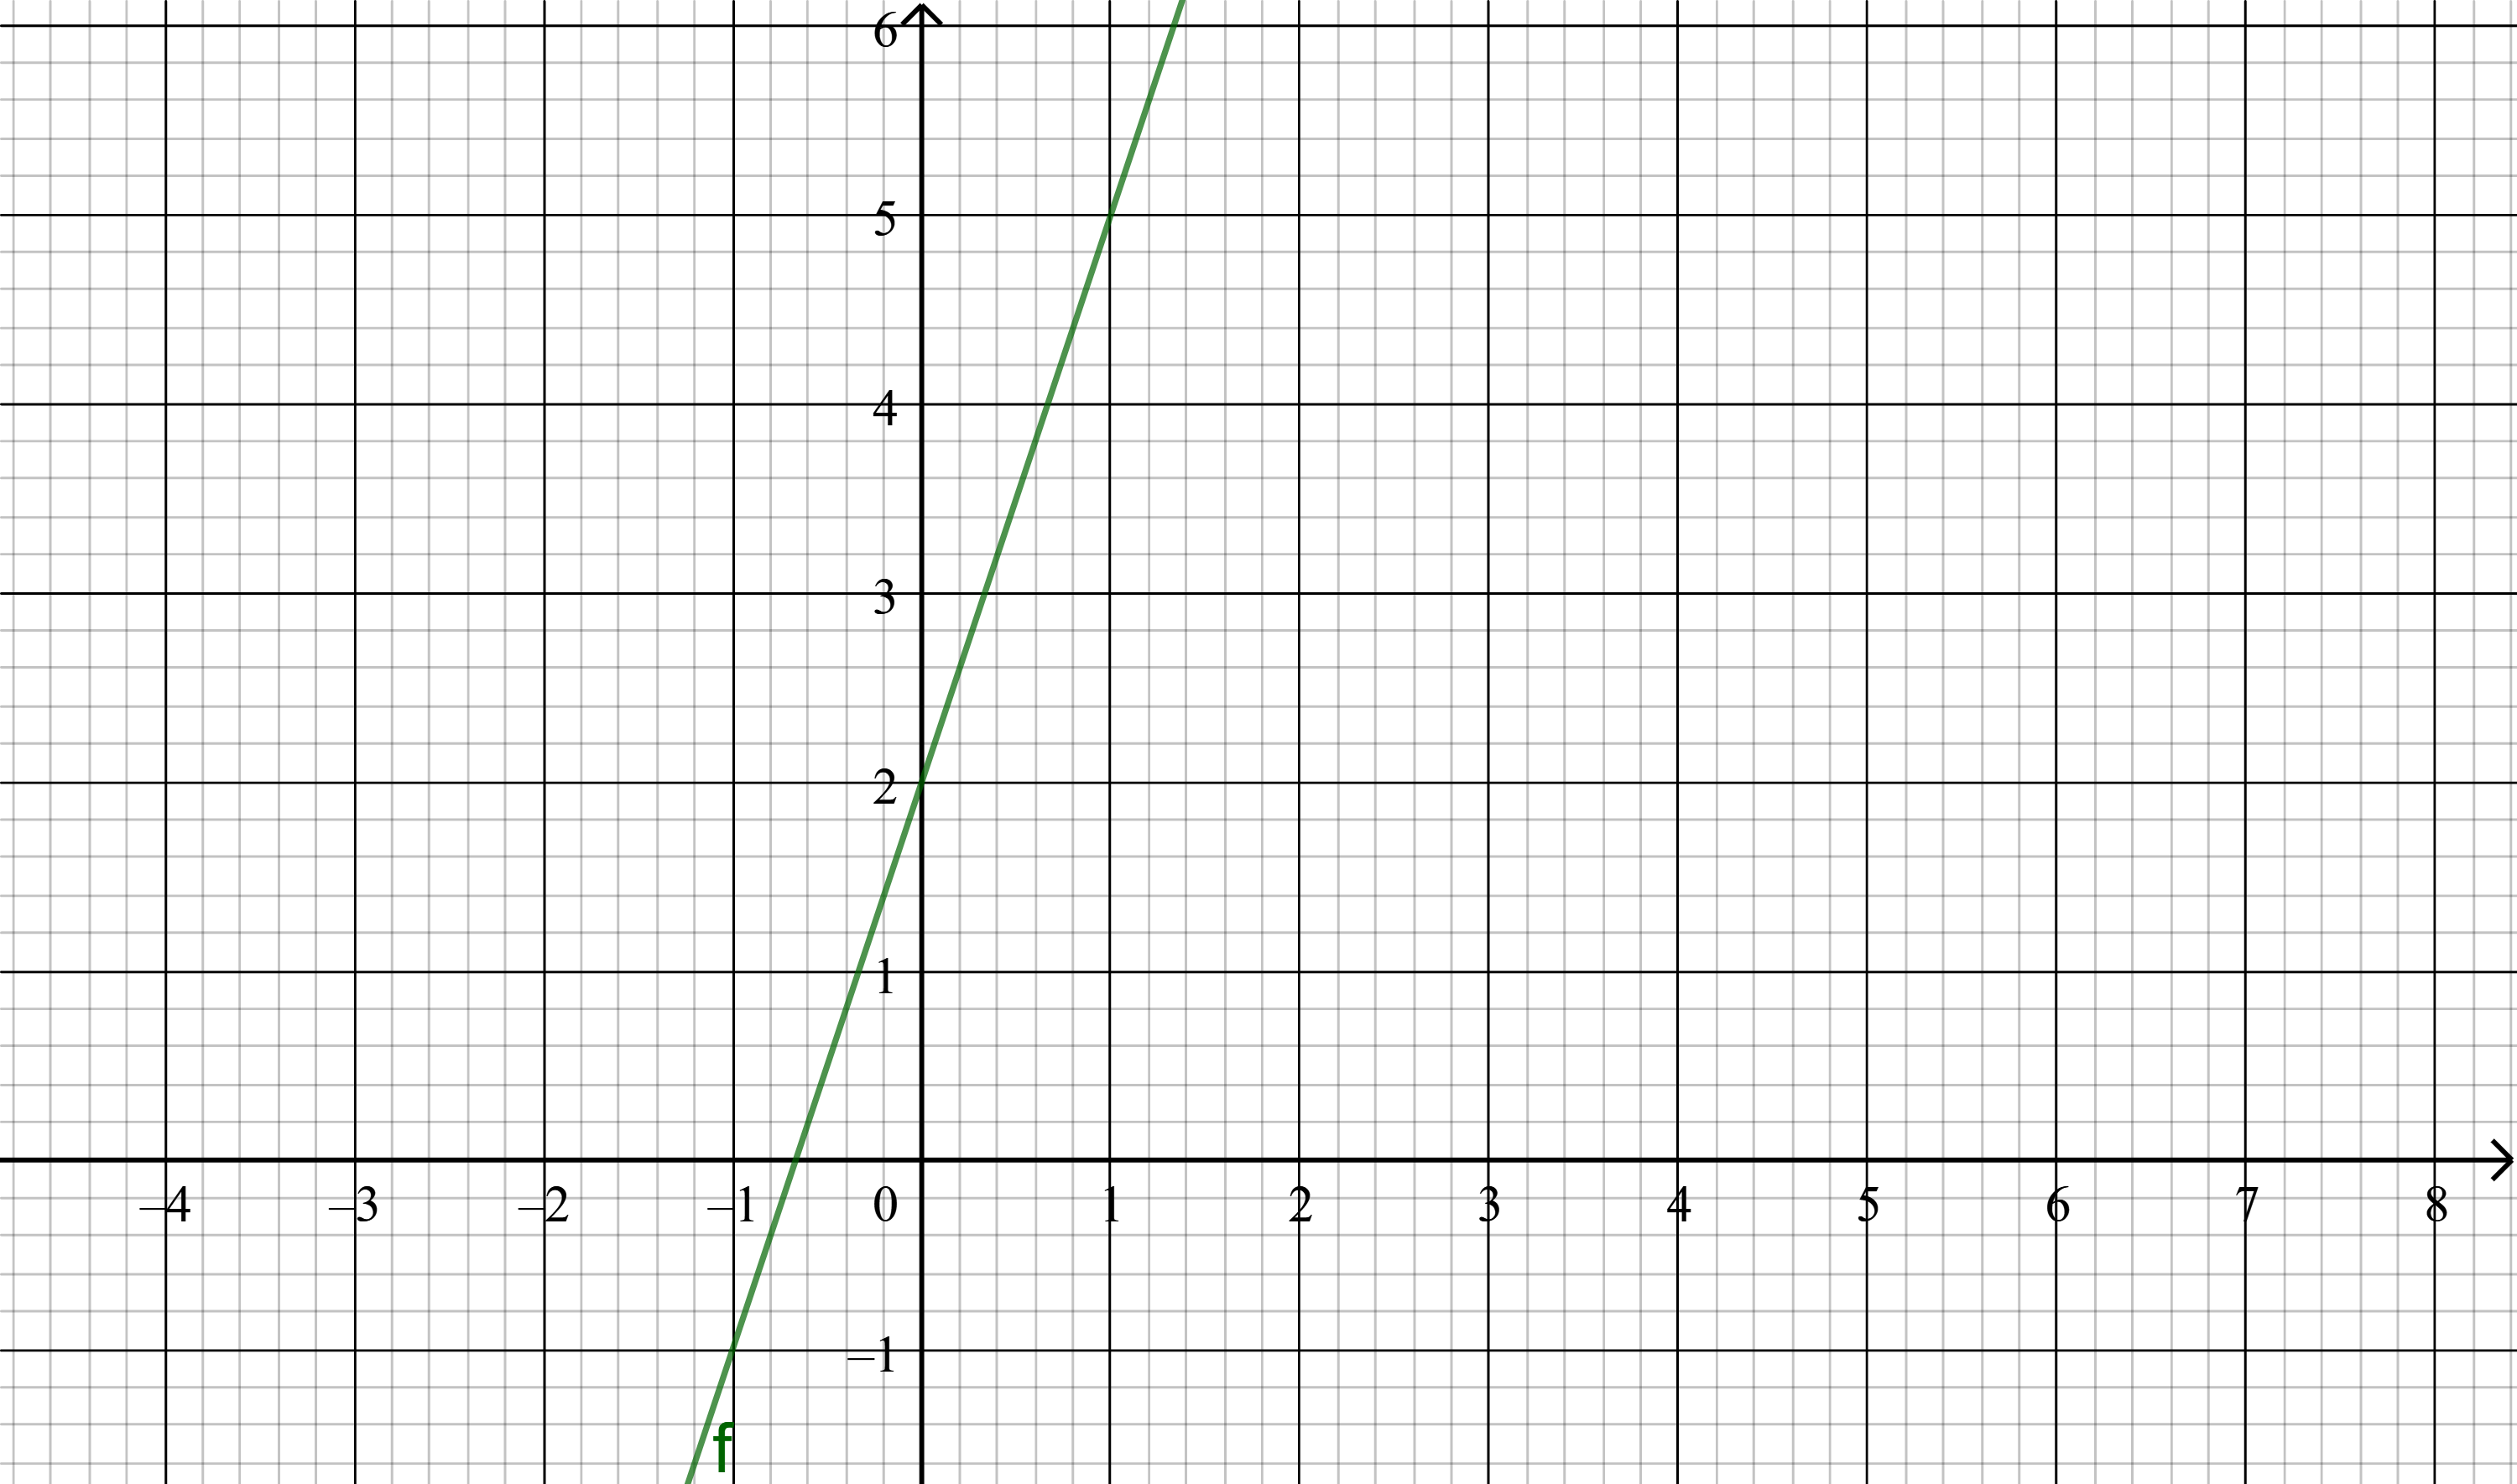
\includegraphics[width=0.5\textwidth]{pics/LinFunktion1}\\
 Bestimme die Funktionsgleichung von f. }
    \solution{ }
    \end{Add}
    \begin{Add}{MaI}{basal1}{LineareFunktionen}{leicht}
    \question{ Gegeben ist der Graph der Funktion f. \\
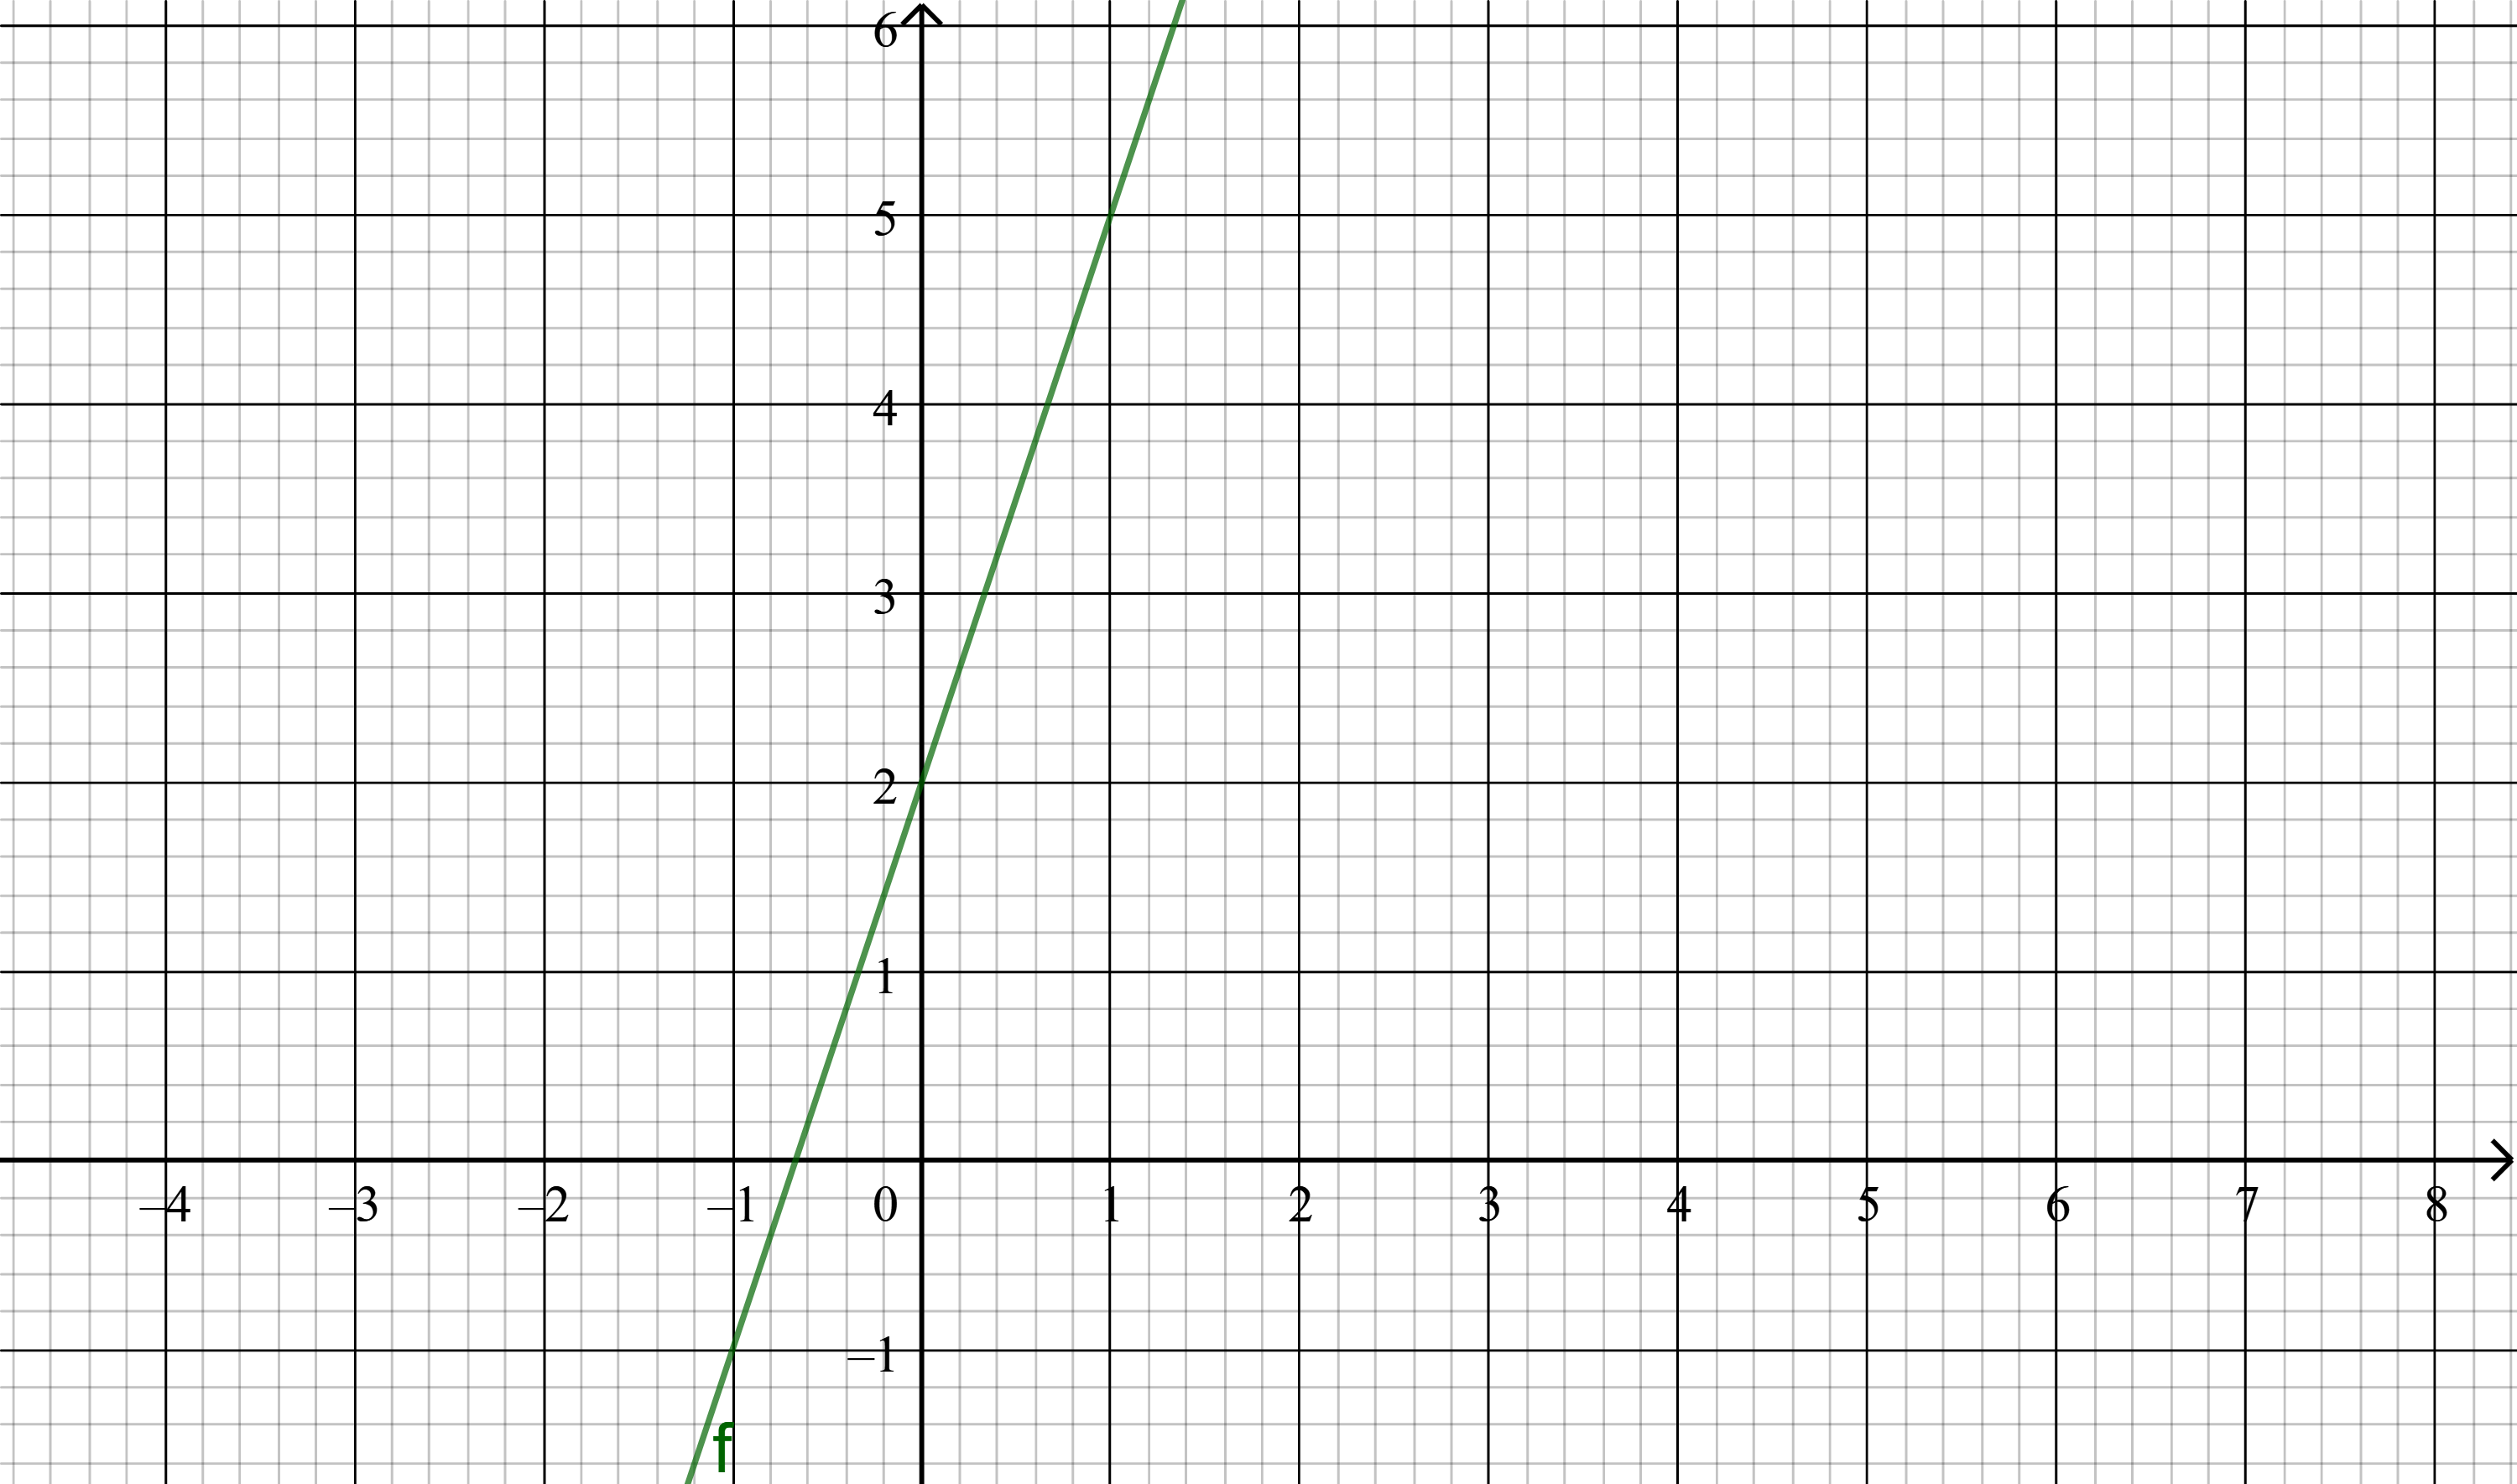
\includegraphics[width=0.5\textwidth]{pics/LinFunktion1}\\
 Bestimme die Funktionsgleichung von f. }
    \solution{ $f(x)=3x+2$ }
    \end{Add}
    

    \begin{Add}{MaI}{basal1}{LineareFunktionen}{leicht}
    \question{ Gegeben ist der Graph der Funktion f. \\
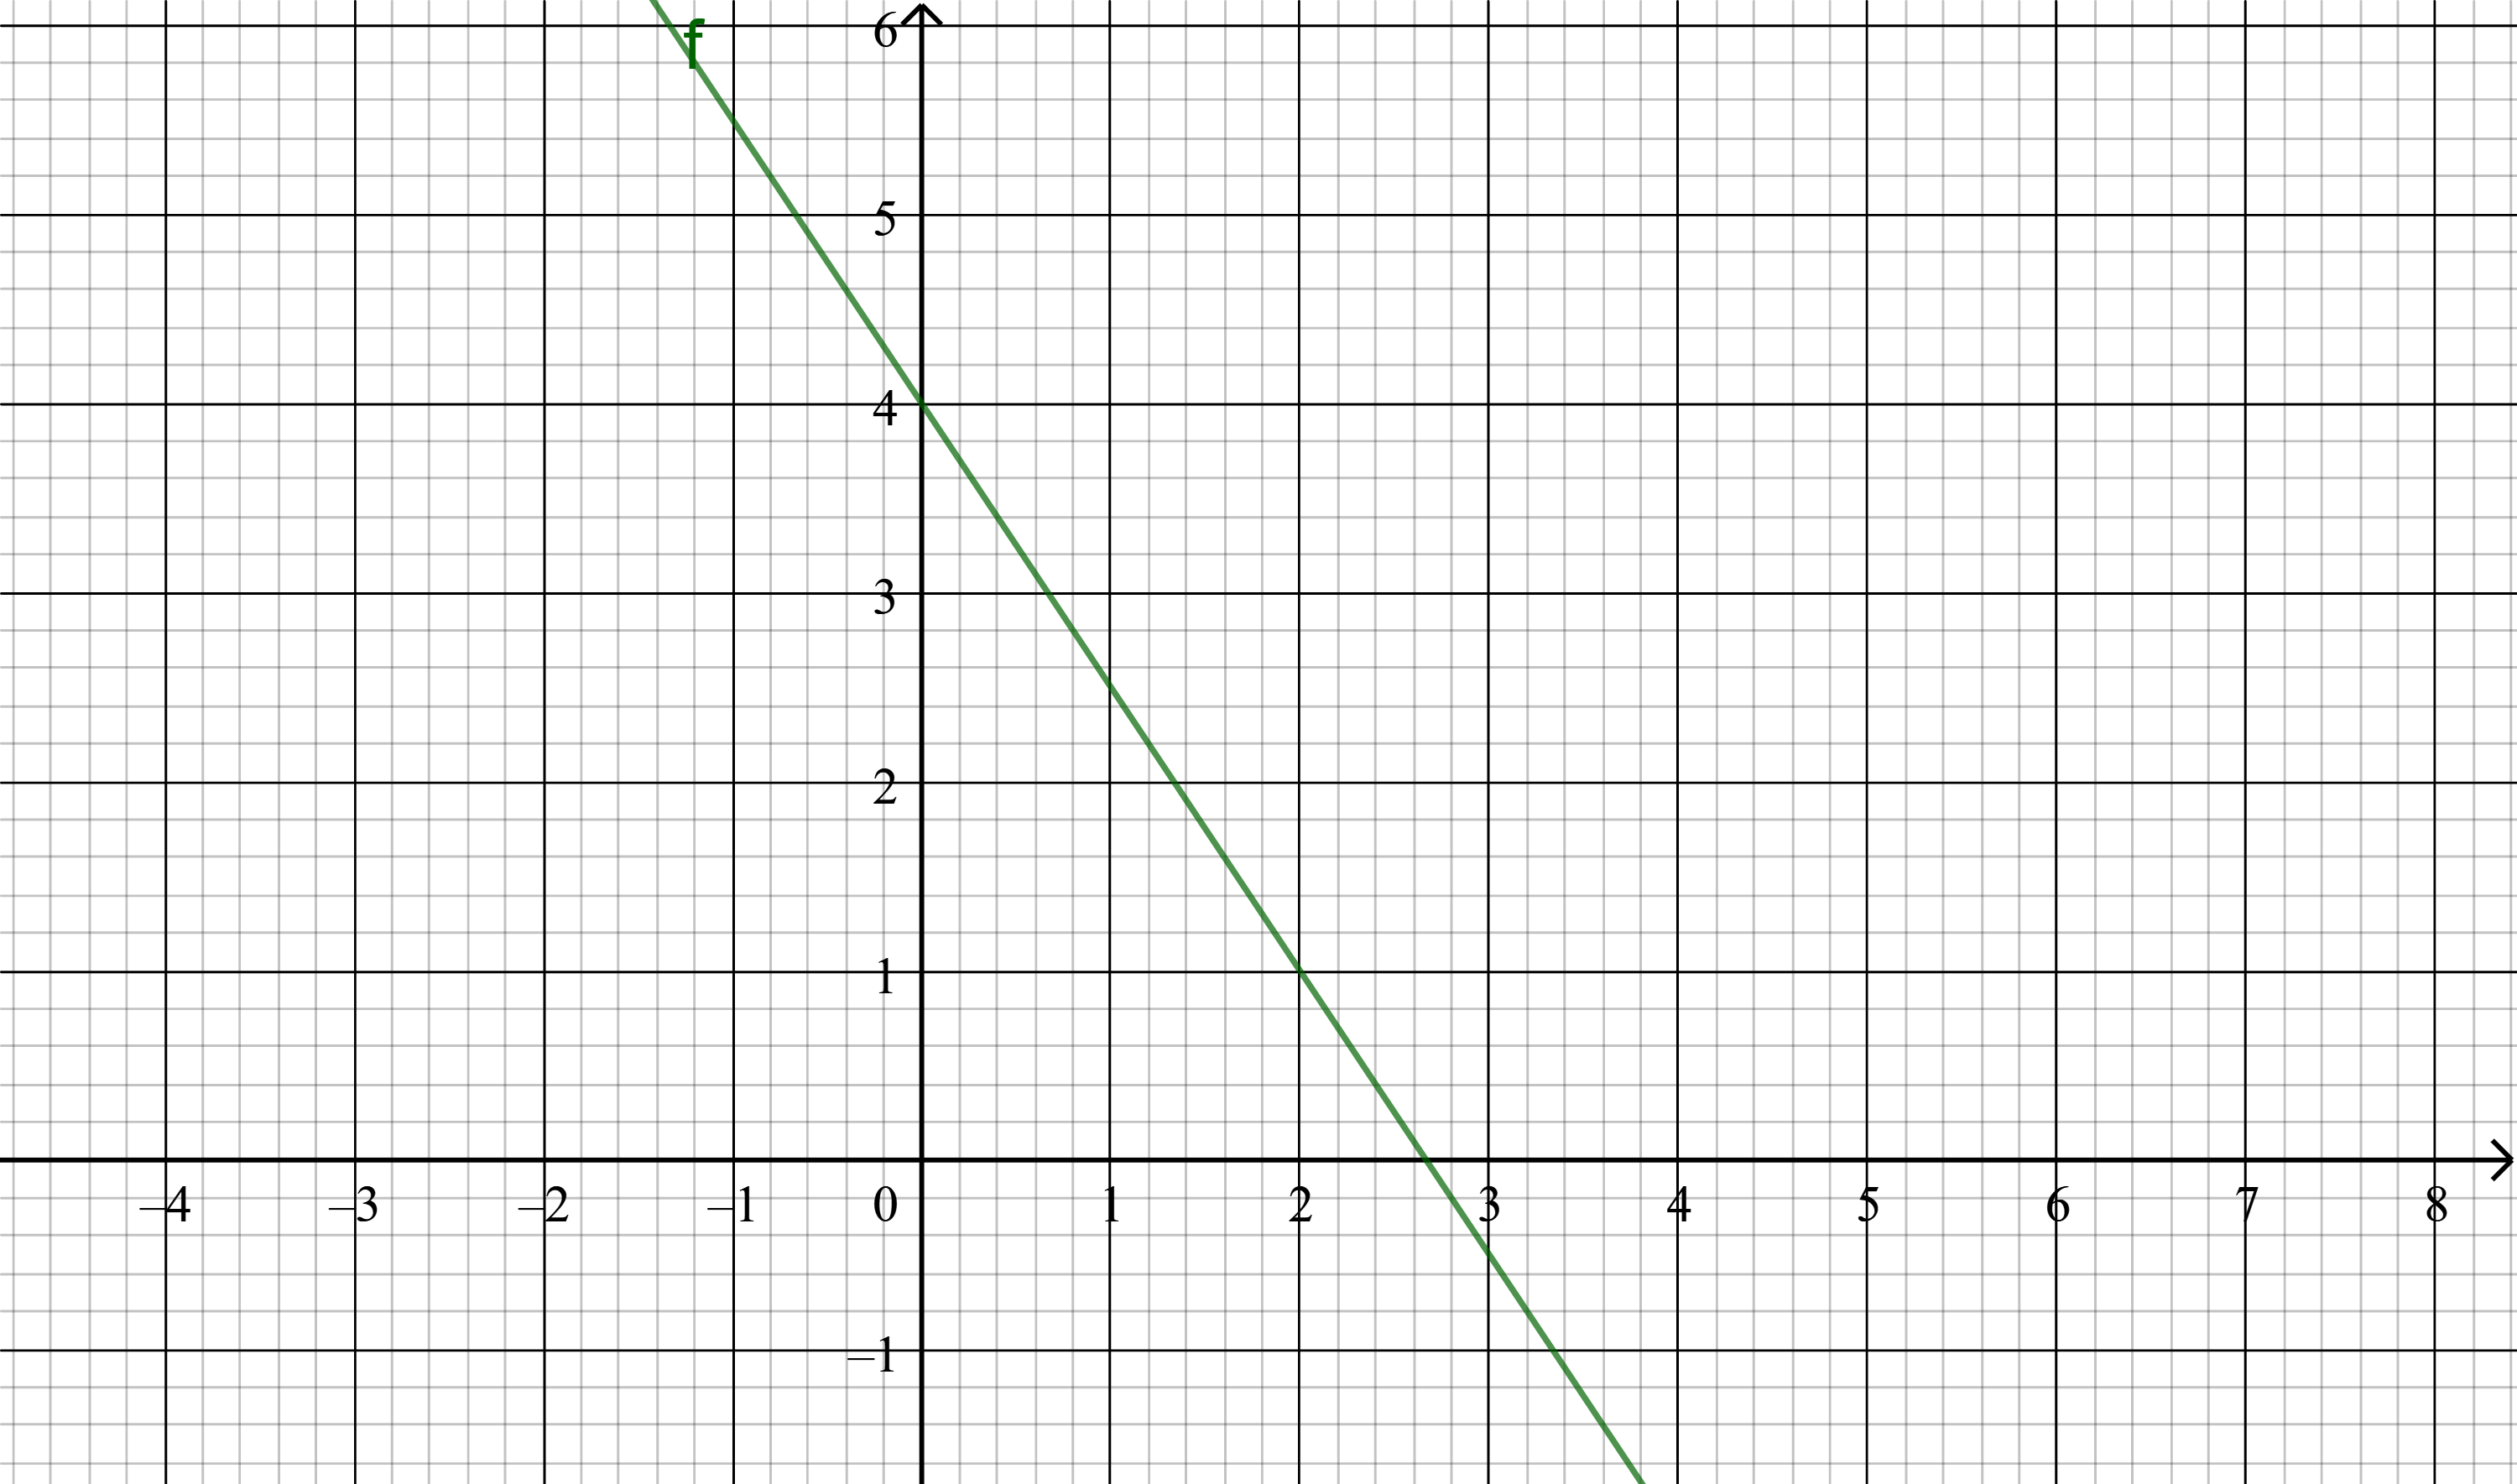
\includegraphics[width=0.5\textwidth]{pics/LinFunktion2}\\
 Bestimme die Funktionsgleichung von f. }
    \solution{ }
    \end{Add}
    \begin{Add}{MaI}{basal1}{LineareFunktionen}{leicht}
    \question{ Gegeben ist der Graph der Funktion f. \\
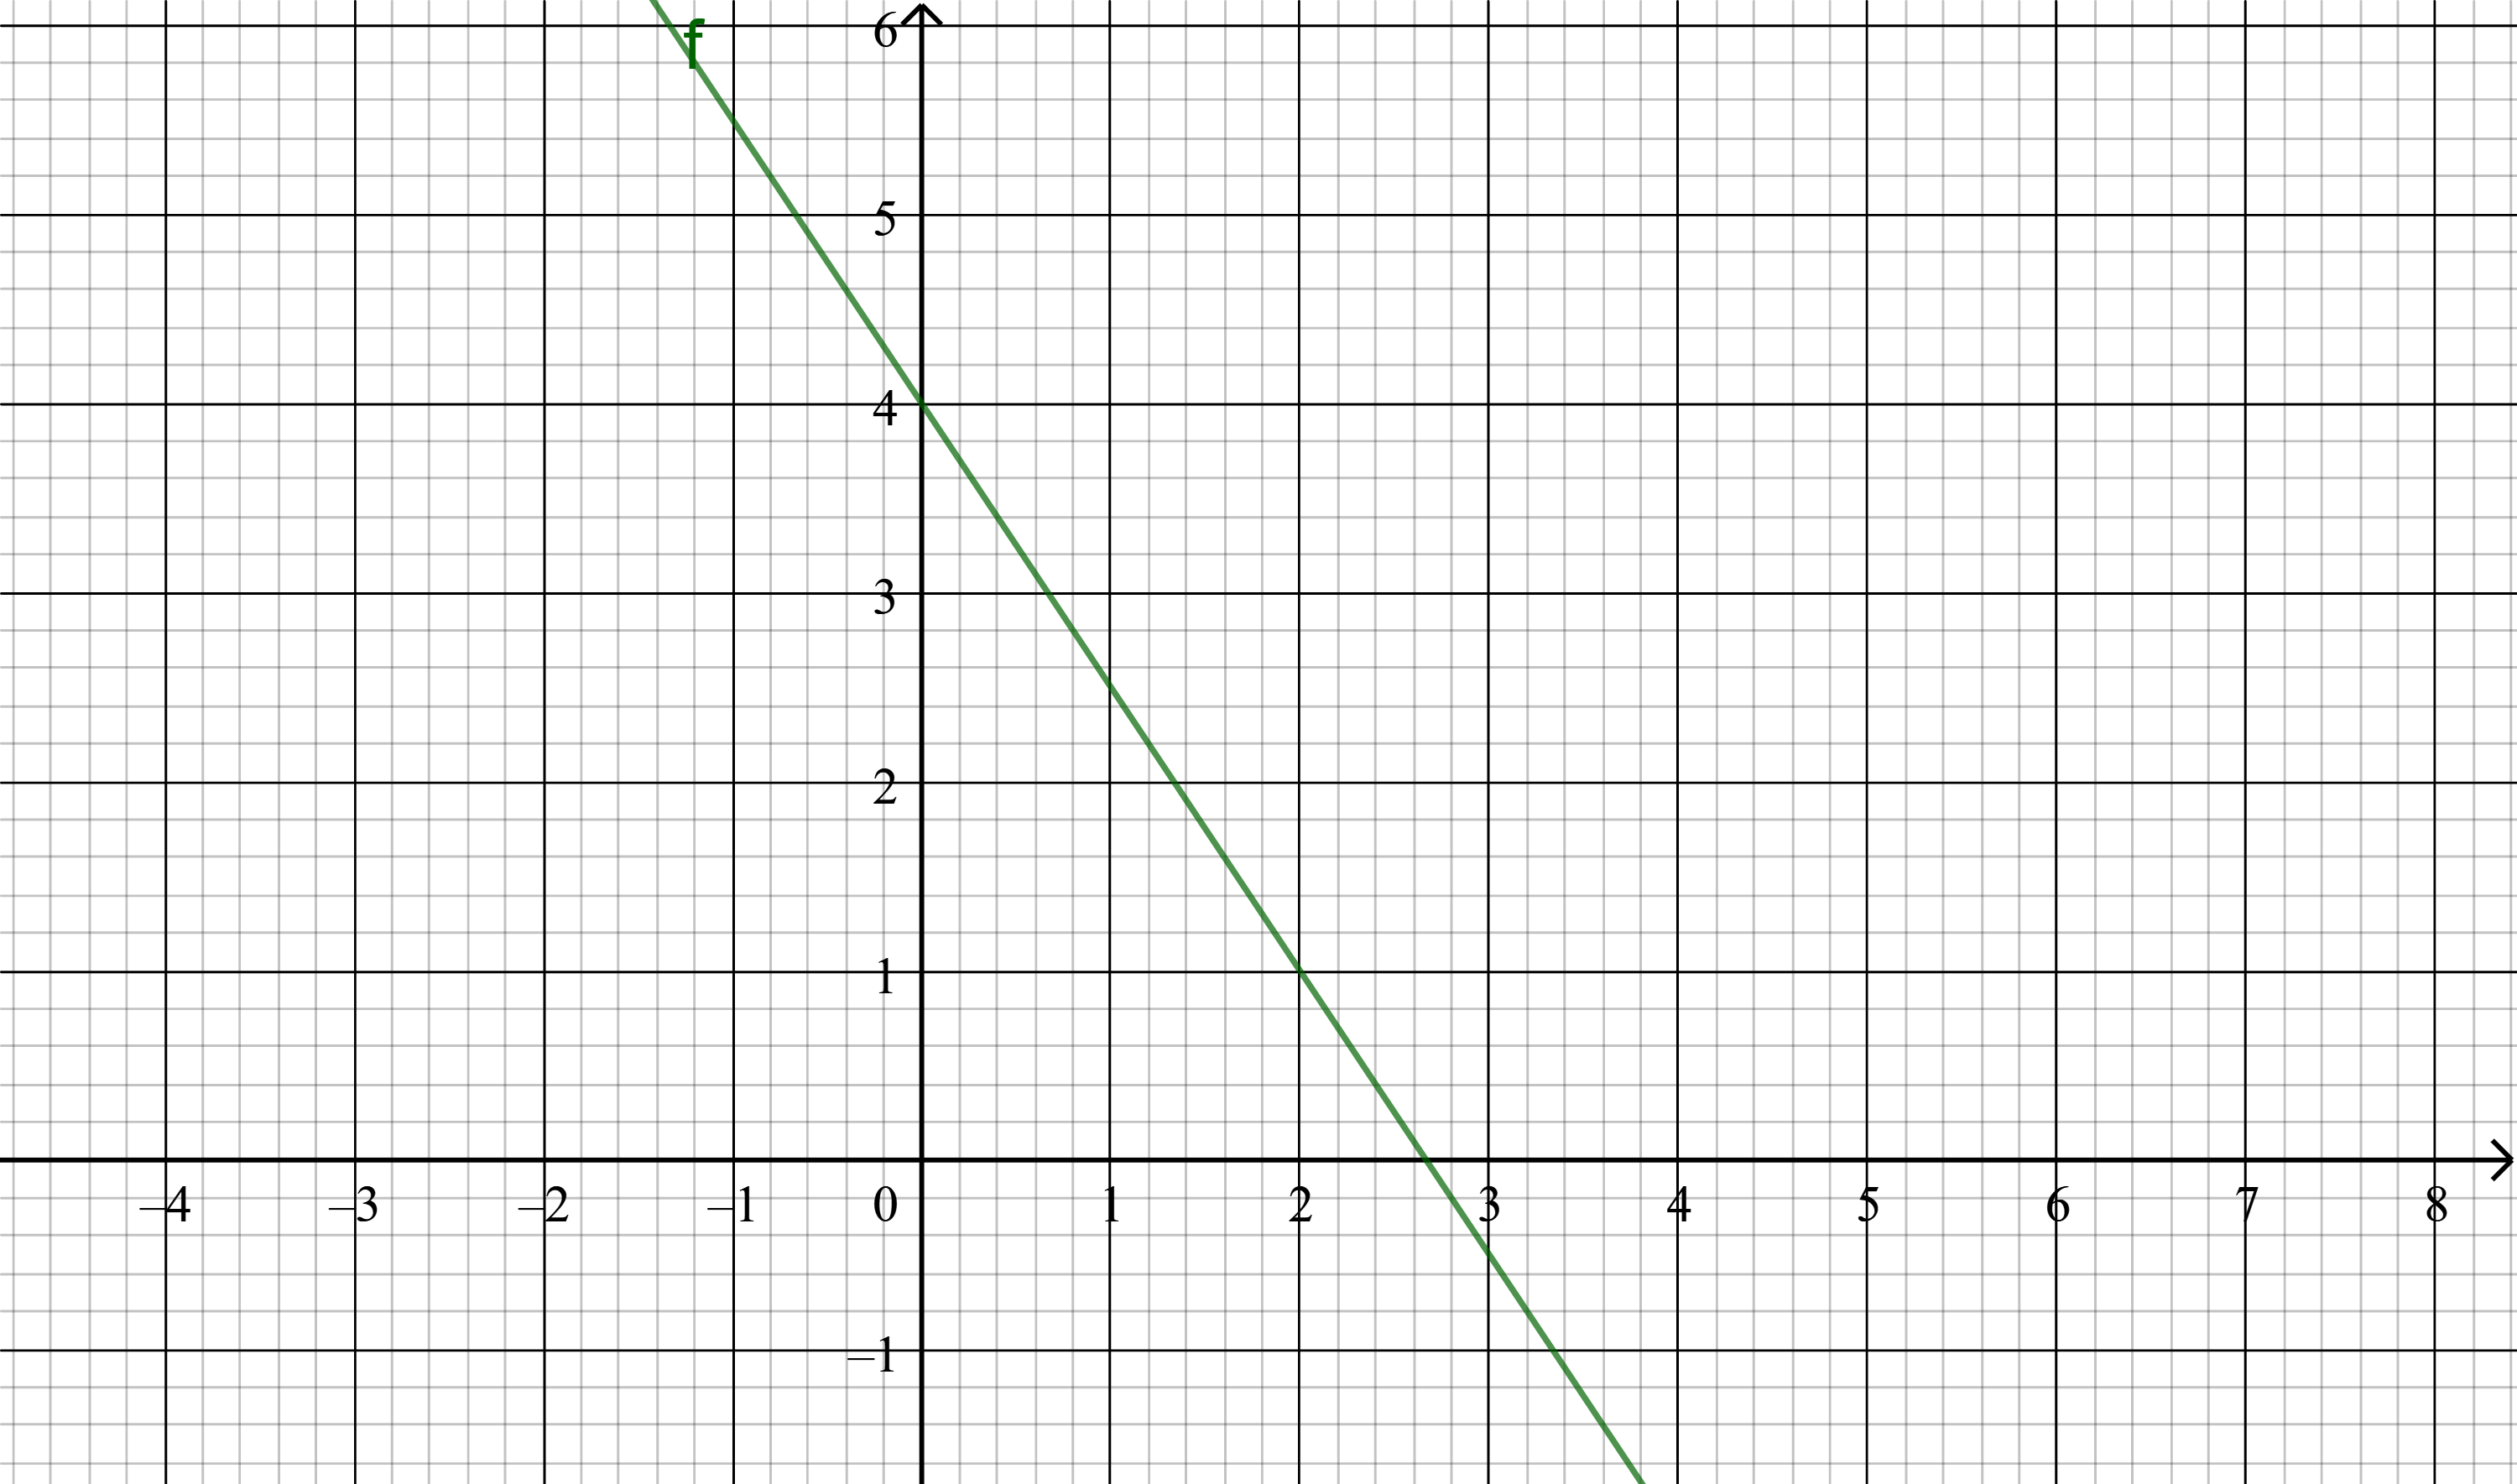
\includegraphics[width=0.5\textwidth]{pics/LinFunktion2}\\
 Bestimme die Funktionsgleichung von f. }
    \solution{ $f(x)=-\frac{3}{2}x+4$ }
    \end{Add}
    

    \begin{Add}{MaI}{basal1}{LineareFunktionen}{leicht}
    \question{ Gegeben ist der Graph der Funktion f. \\
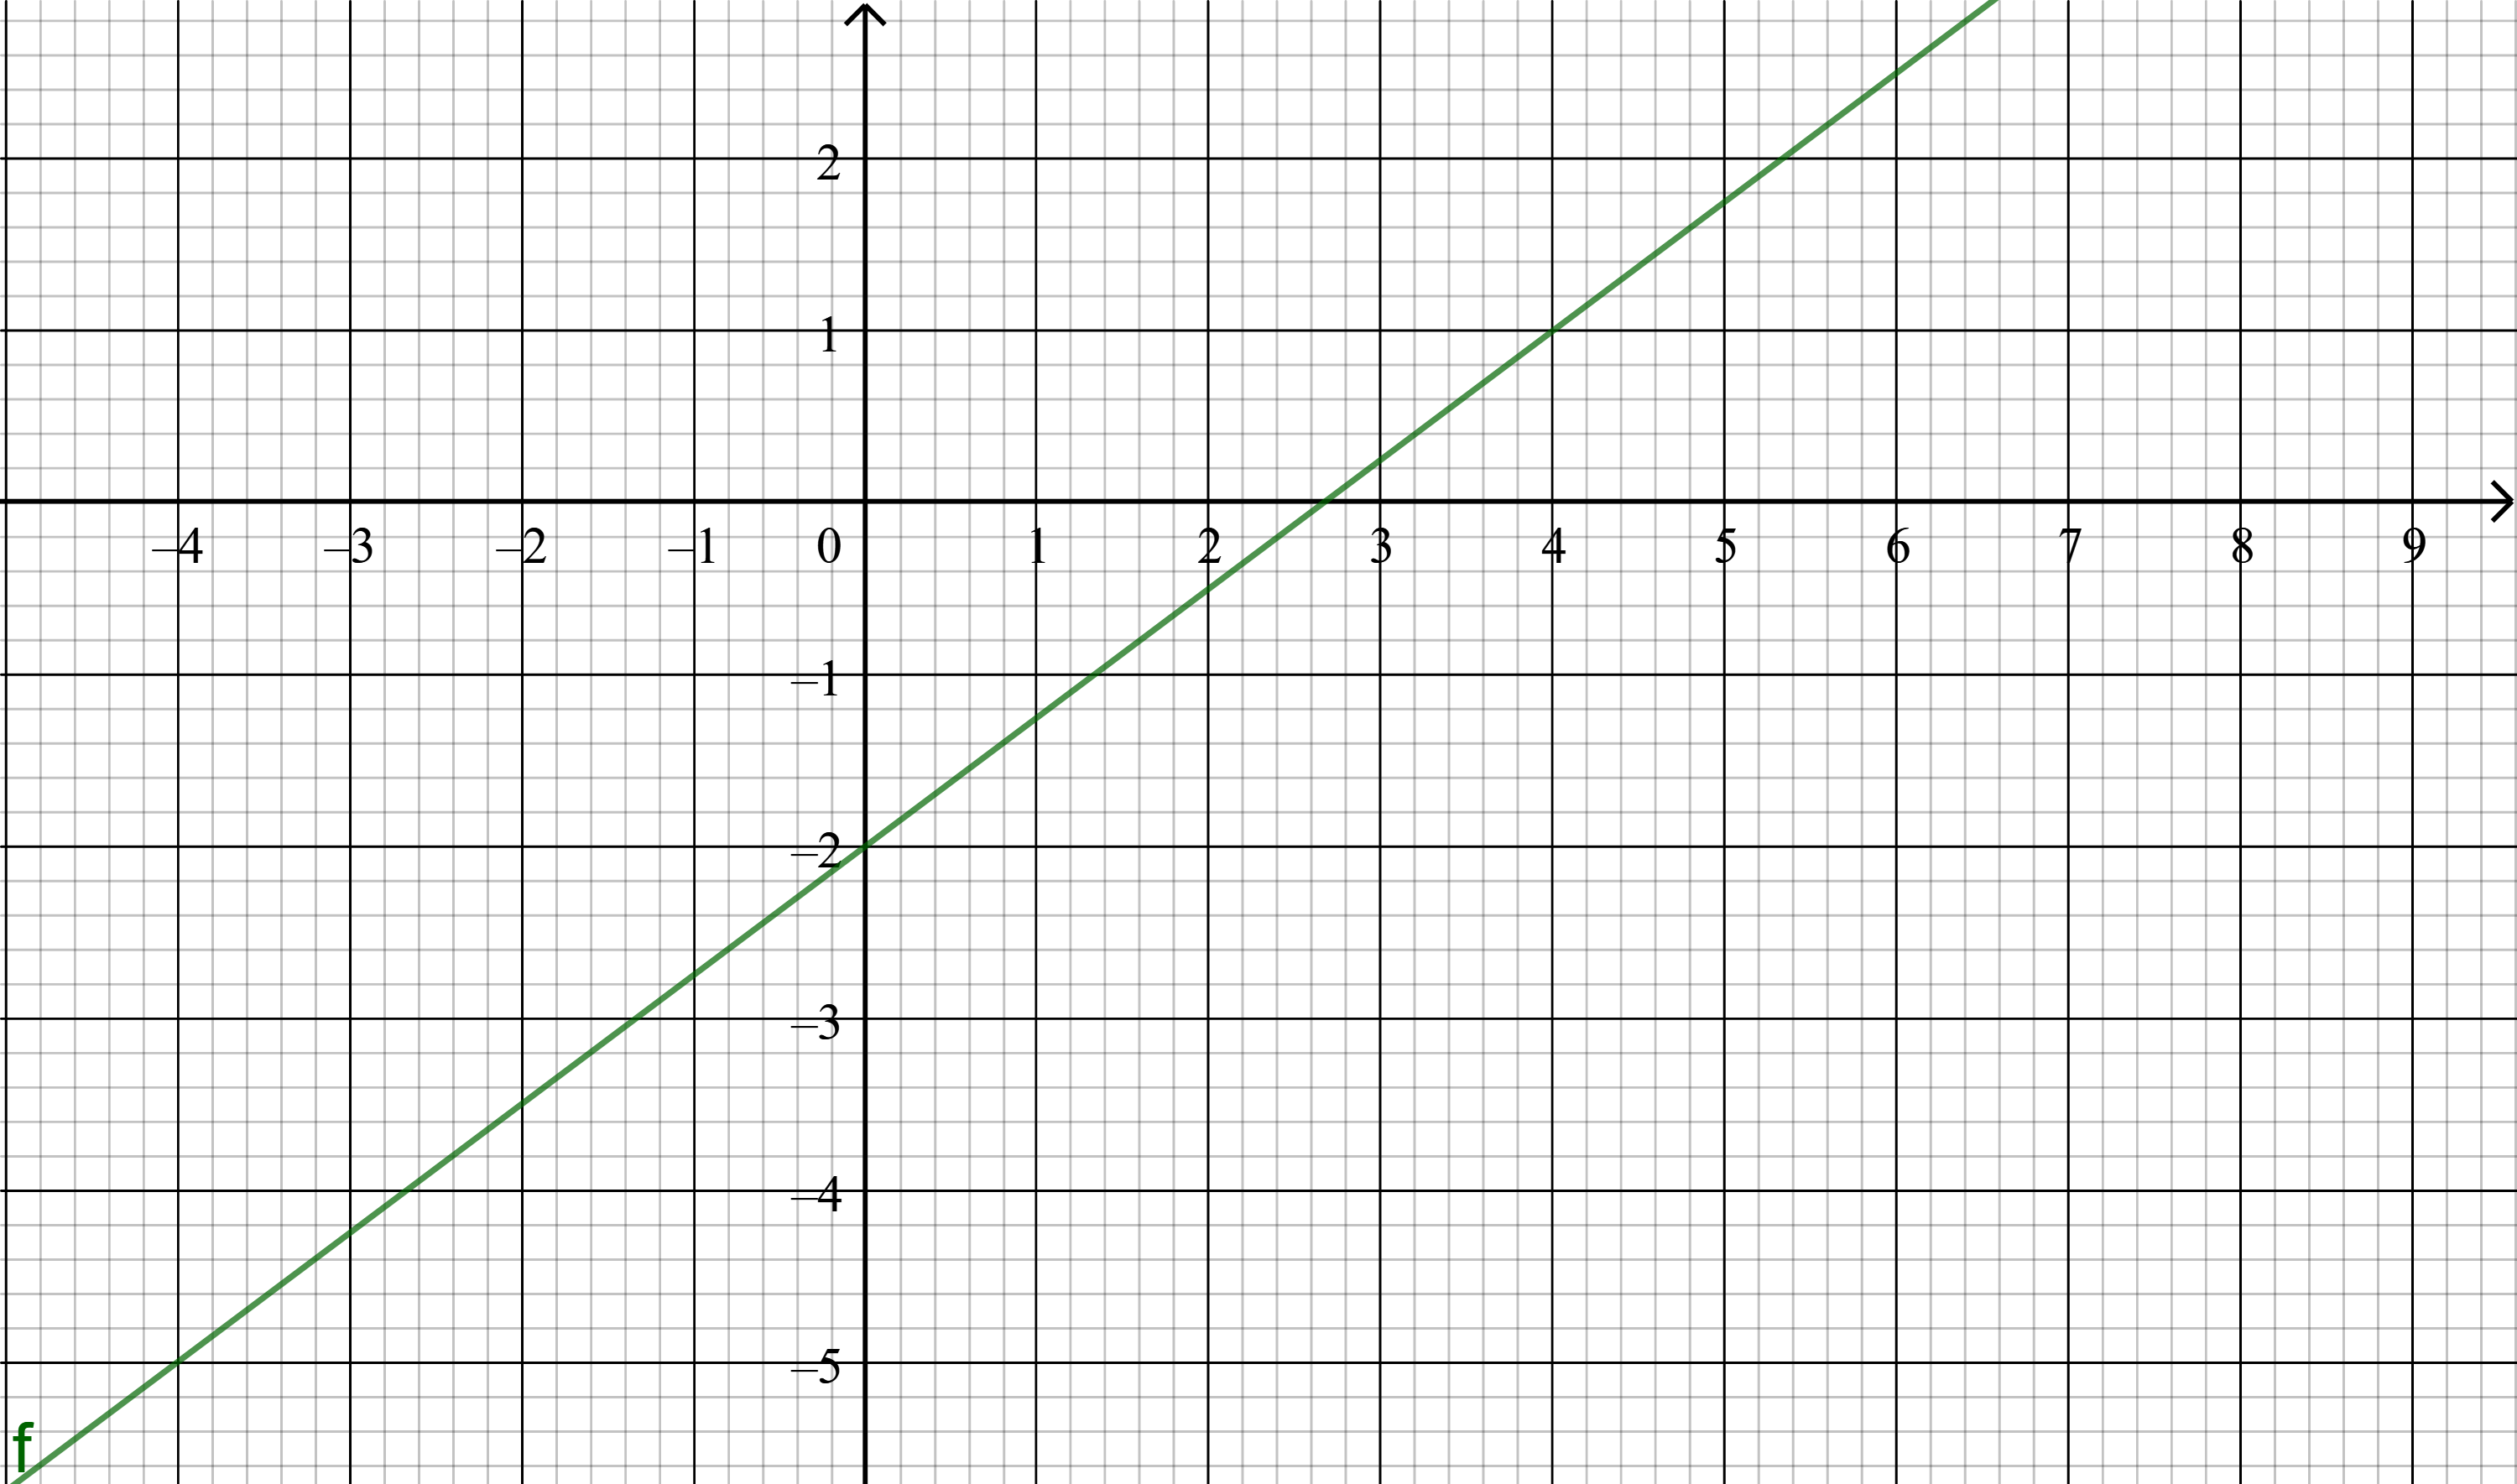
\includegraphics[width=0.5\textwidth]{pics/LinFunktion3}\\
 Bestimme die Funktionsgleichung von f. }
    \solution{ }
    \end{Add}
    \begin{Add}{MaI}{basal1}{LineareFunktionen}{leicht}
    \question{ Gegeben ist der Graph der Funktion f. \\
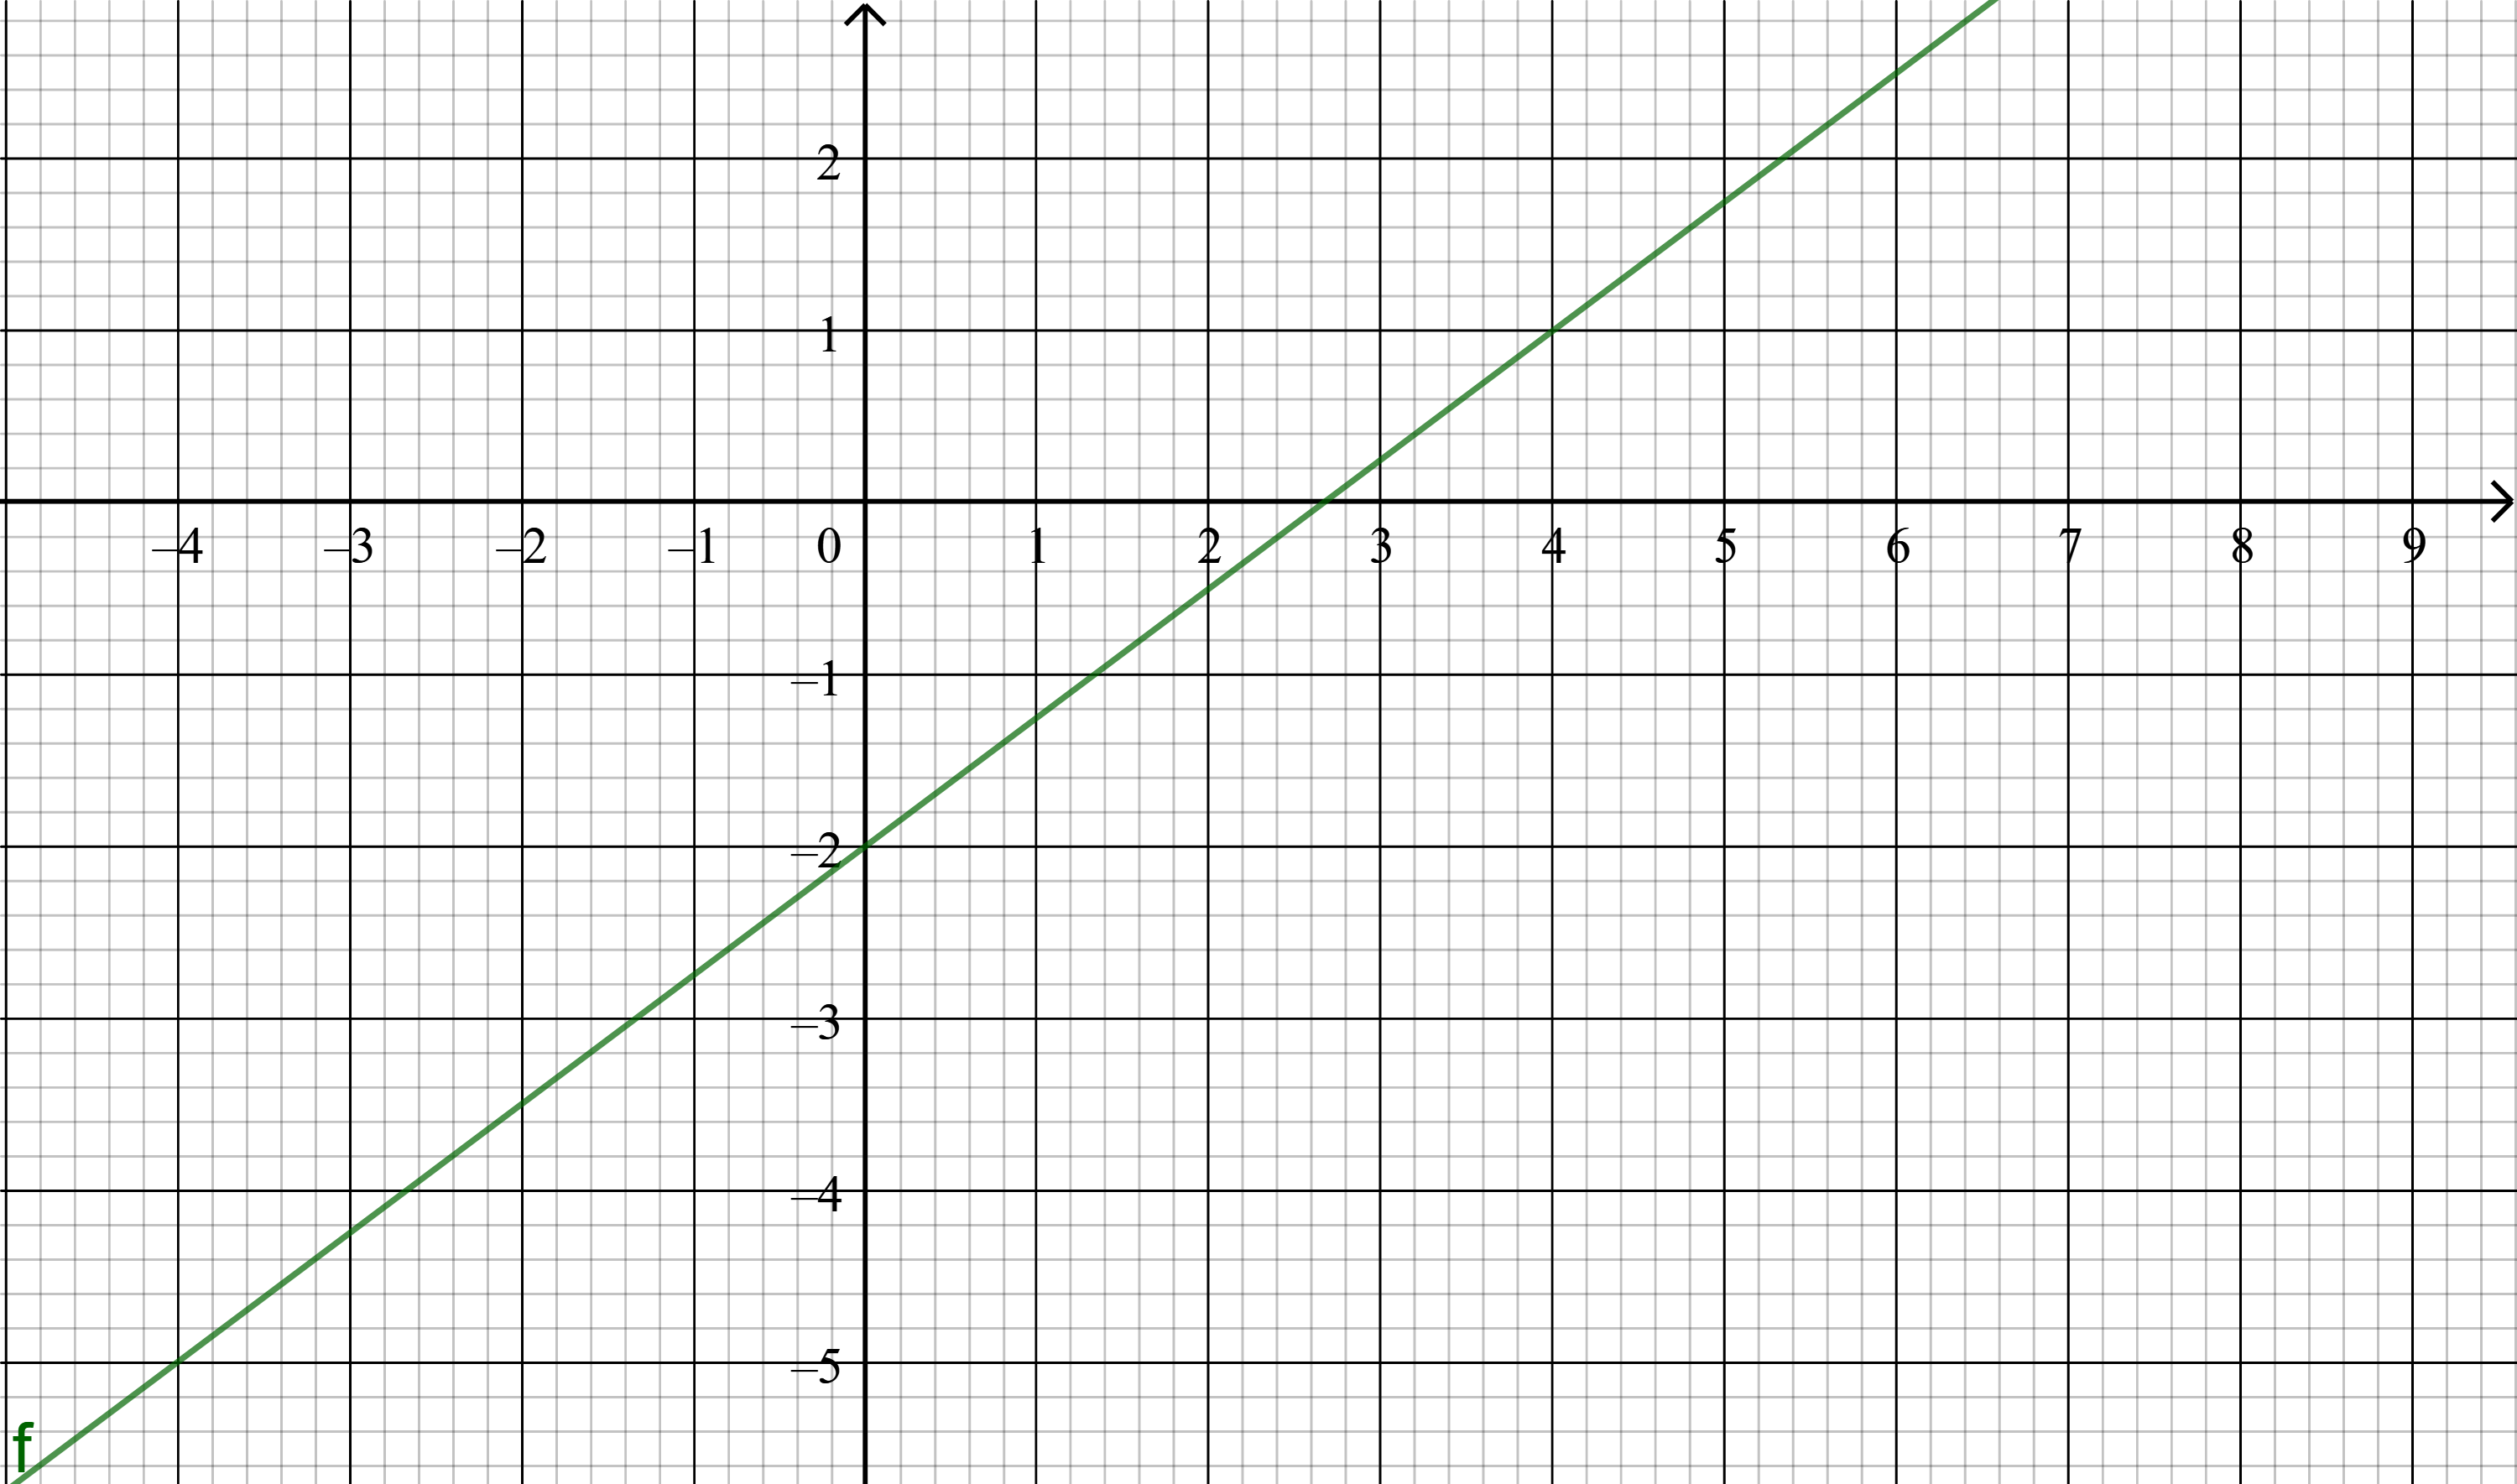
\includegraphics[width=0.5\textwidth]{pics/LinFunktion3}\\
 Bestimme die Funktionsgleichung von f. }
    \solution{ $f(x)=\frac{3}{4}x-2$ }
    \end{Add}
    

    \begin{Add}{MaI}{basal1}{LineareFunktionen}{leicht}
    \question{ Gegeben ist der Graph der Funktion f. \\
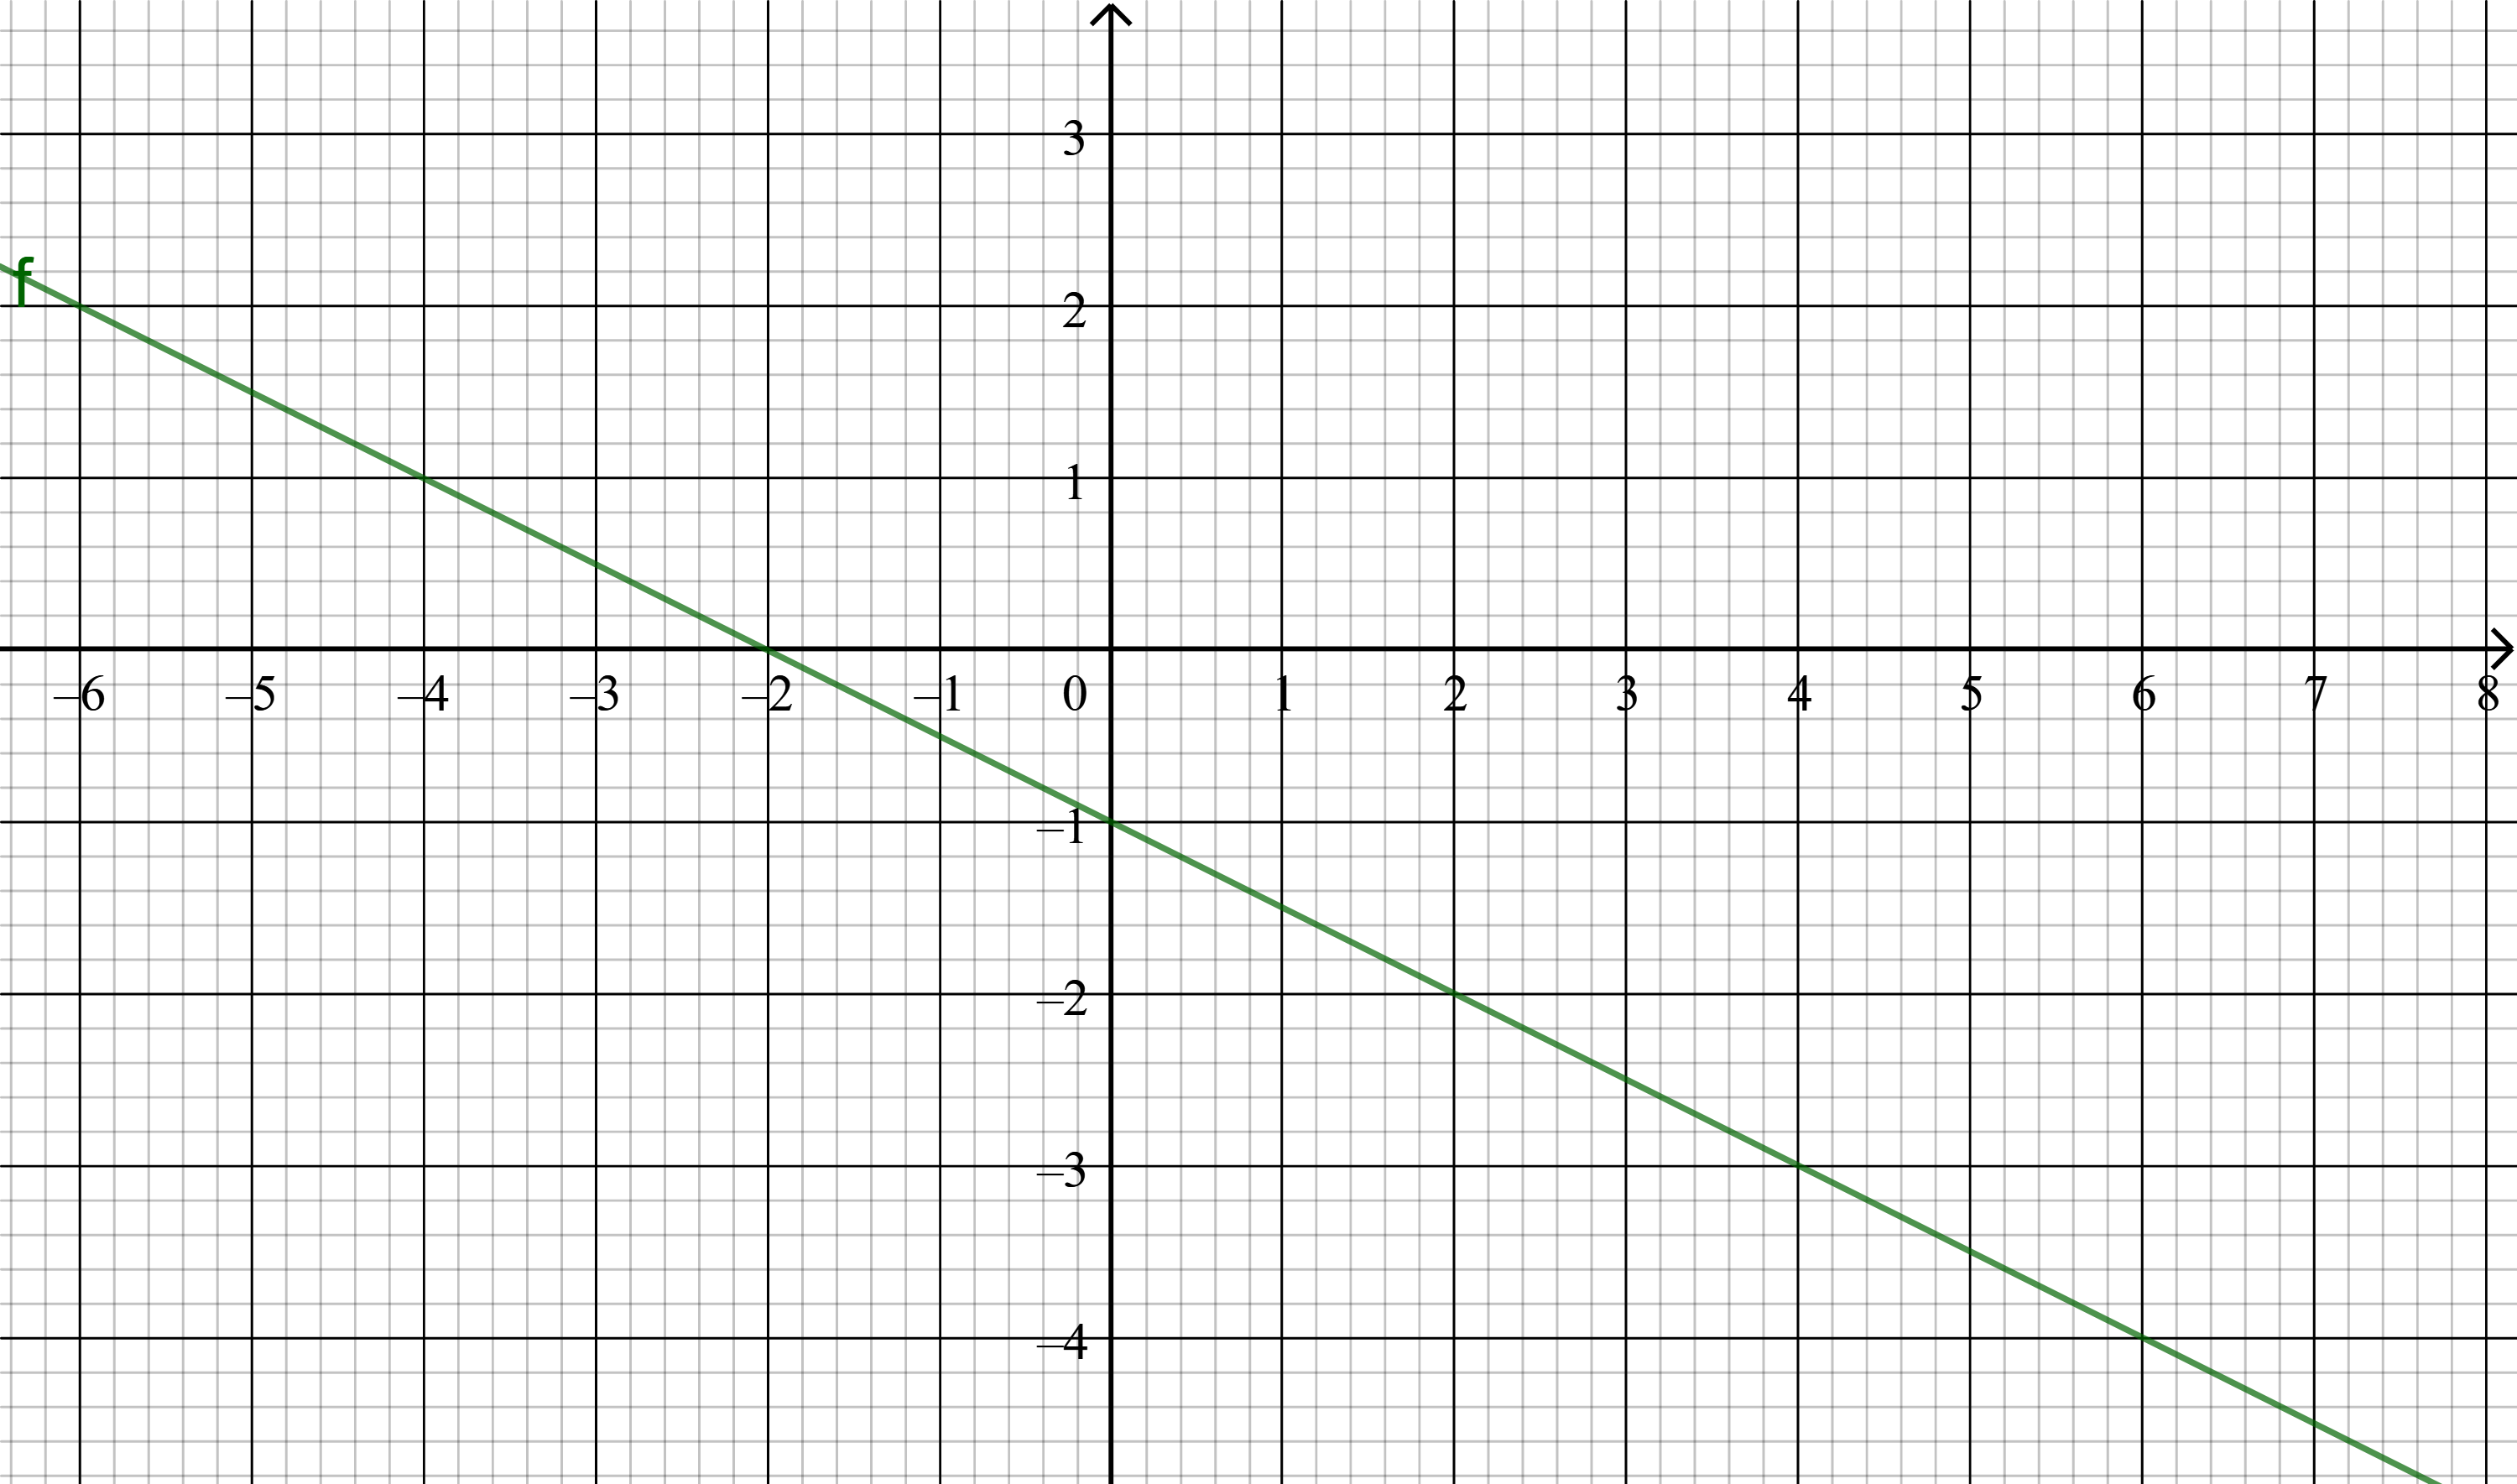
\includegraphics[width=0.5\textwidth]{pics/LinFunktion4}\\
 Bestimme die Funktionsgleichung von f. }
    \solution{ }
    \end{Add}
    \begin{Add}{MaI}{basal1}{LineareFunktionen}{leicht}
    \question{ Gegeben ist der Graph der Funktion f. \\
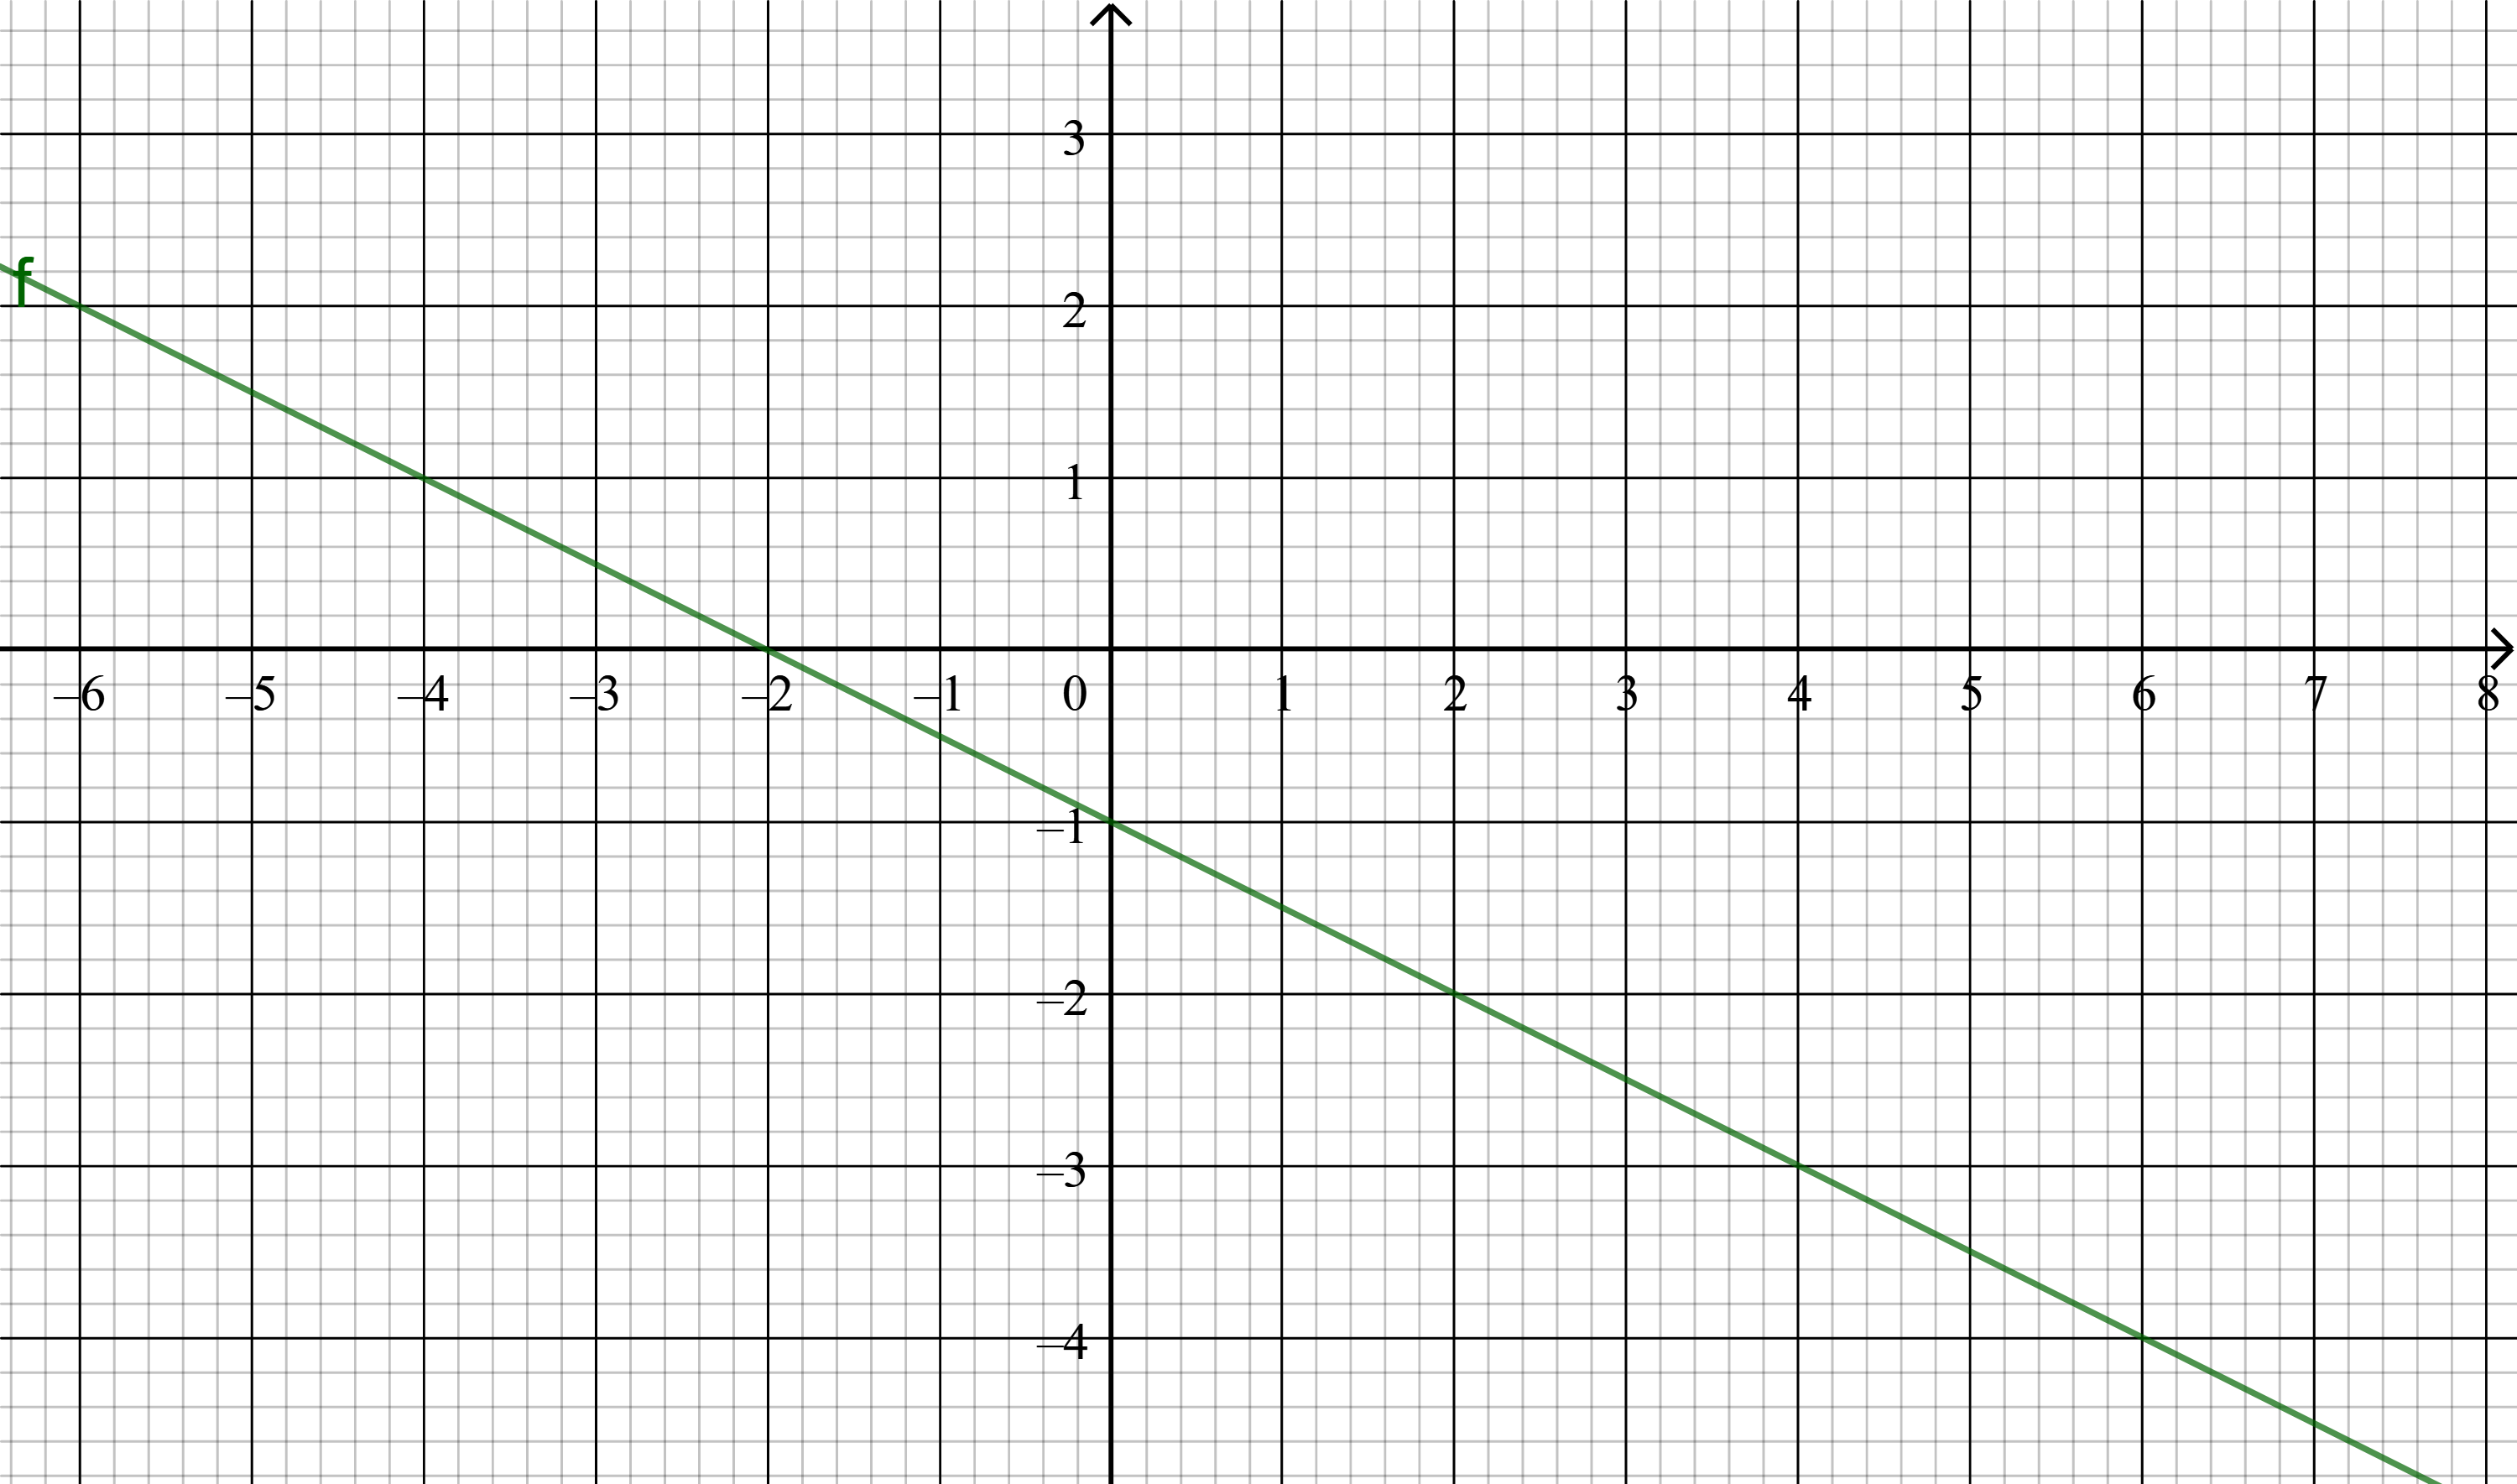
\includegraphics[width=0.5\textwidth]{pics/LinFunktion4}\\
 Bestimme die Funktionsgleichung von f. }
    \solution{ $f(x)=-\frac{1}{2}x-1$ }
    \end{Add}
    

    \begin{Add}{MaI}{basal1}{LineareFunktionen}{leicht}
    \question{ Gegeben ist der Graph der Funktion f. \\
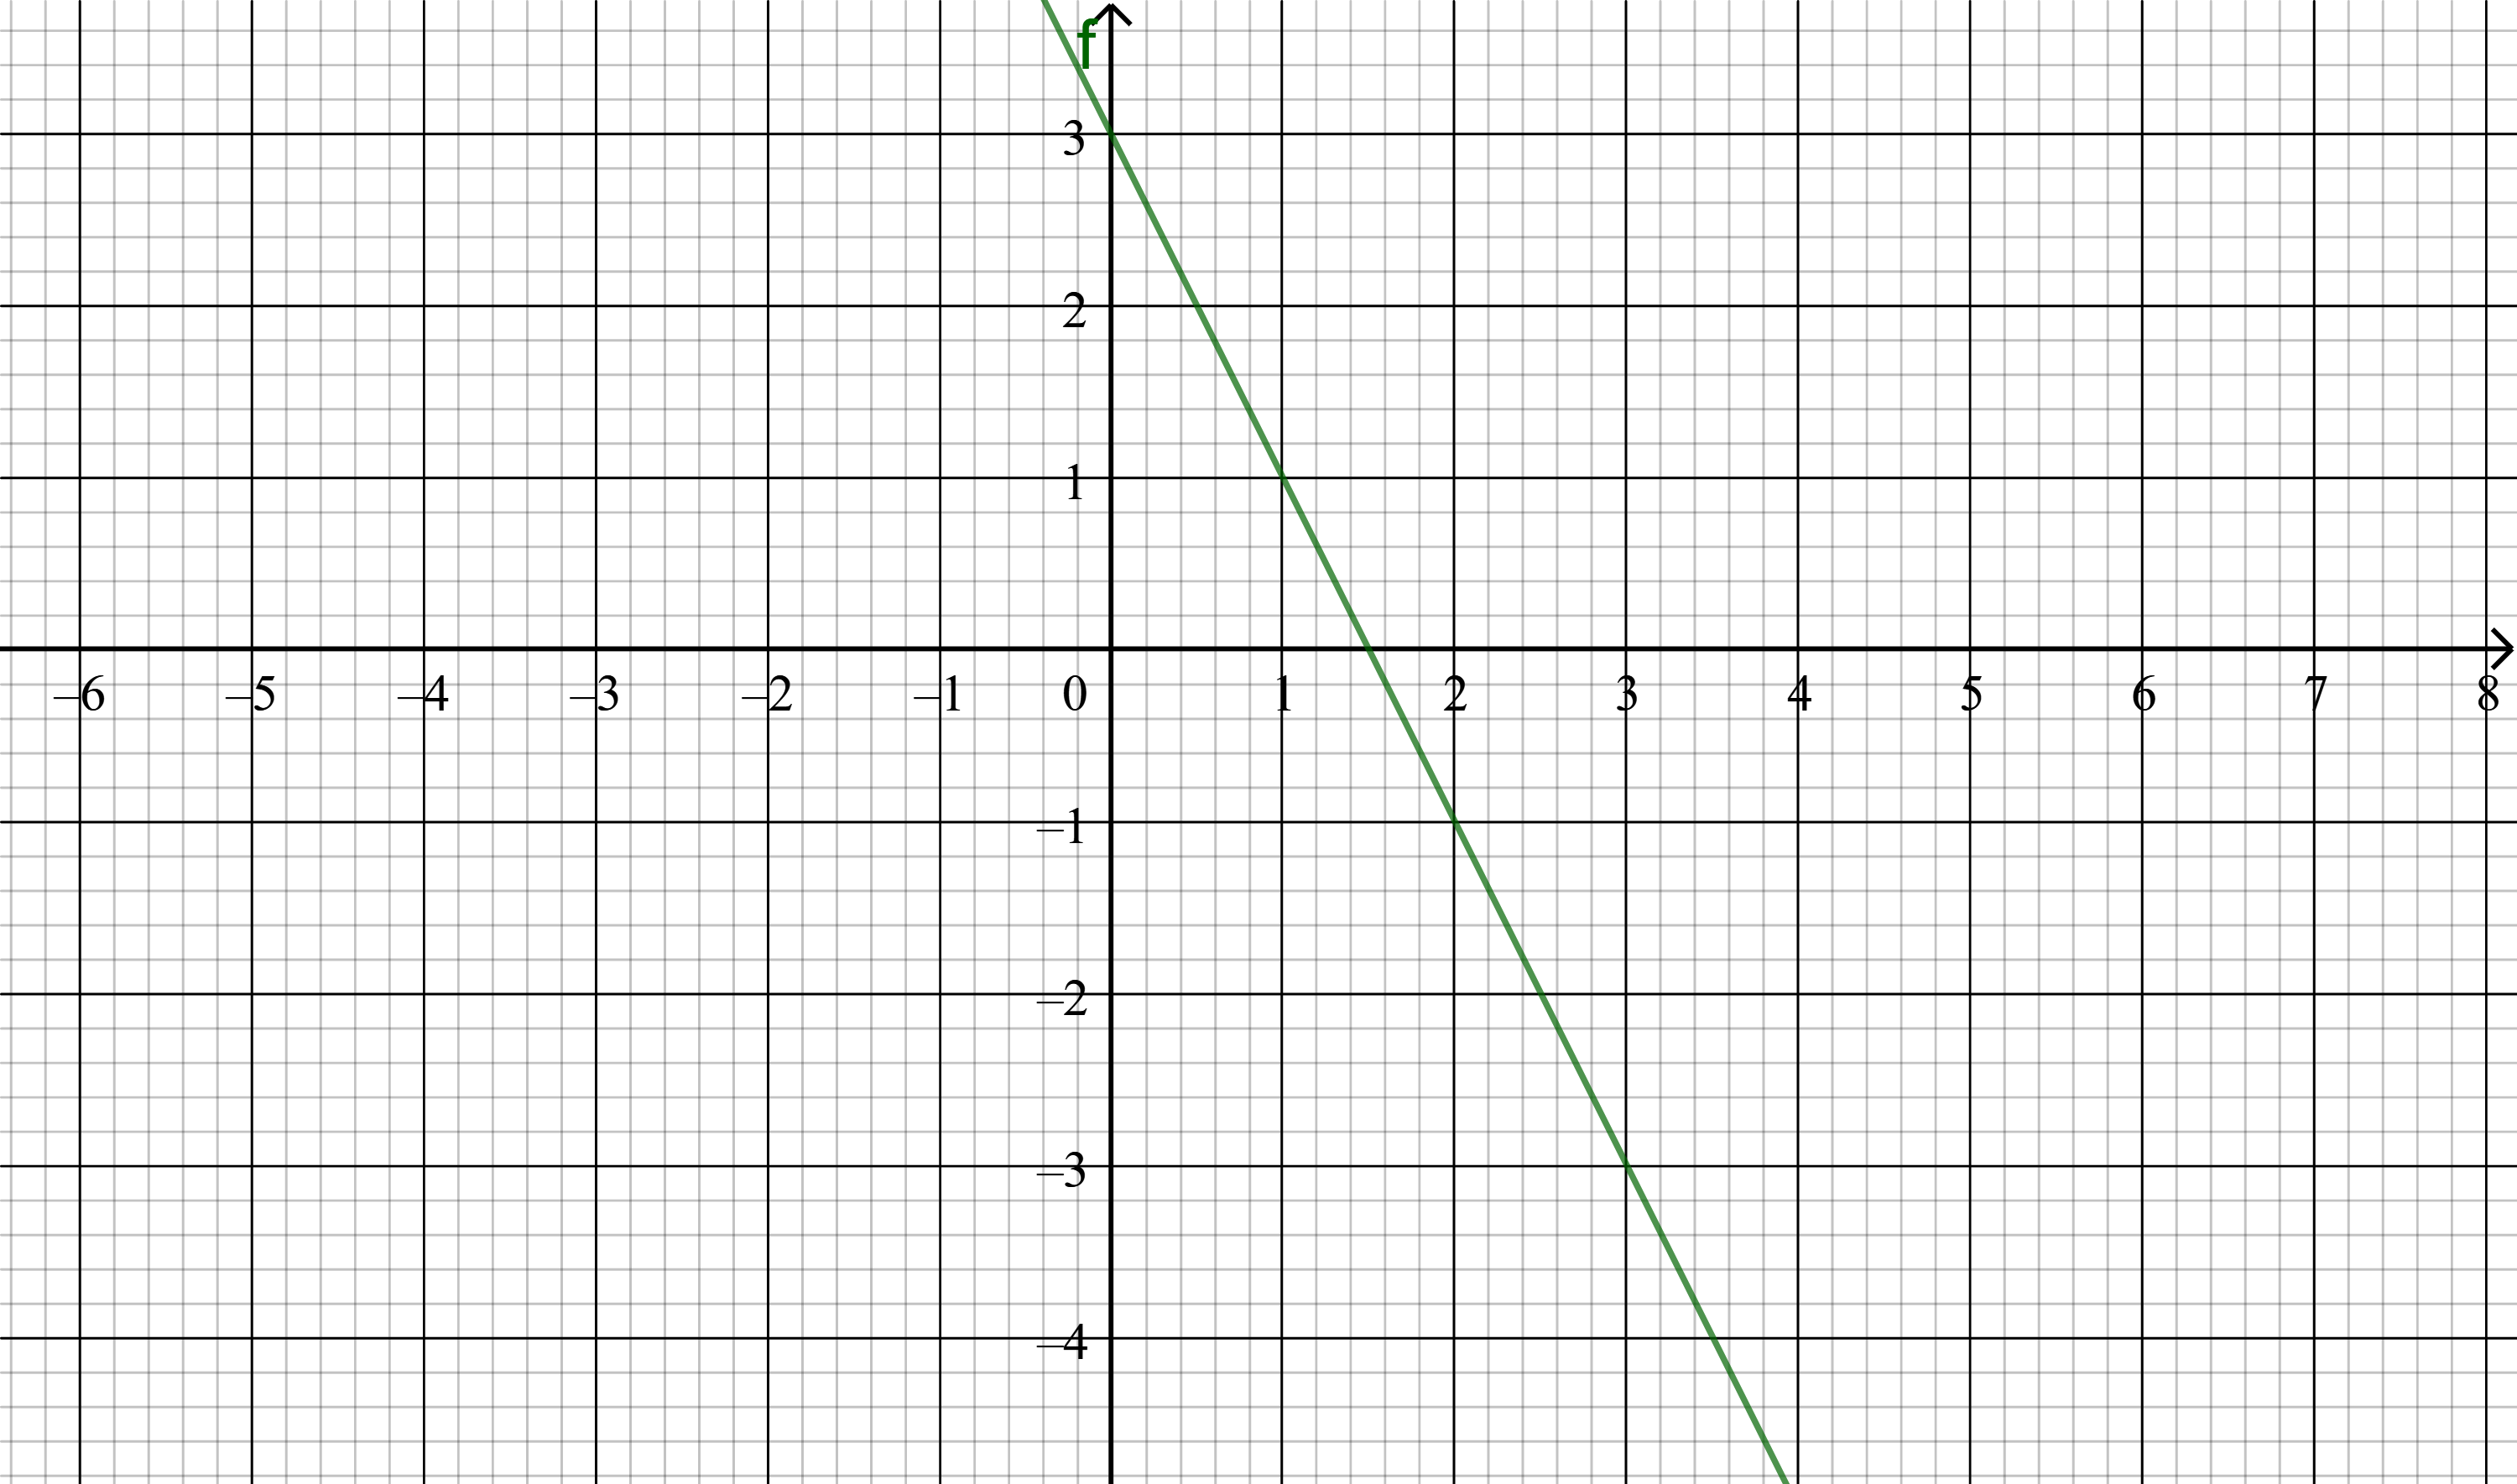
\includegraphics[width=0.5\textwidth]{pics/LinFunktion5}\\
 Bestimme die Funktionsgleichung von f. }
    \solution{ }
    \end{Add}
    \begin{Add}{MaI}{basal1}{LineareFunktionen}{leicht}
    \question{ Gegeben ist der Graph der Funktion f. \\
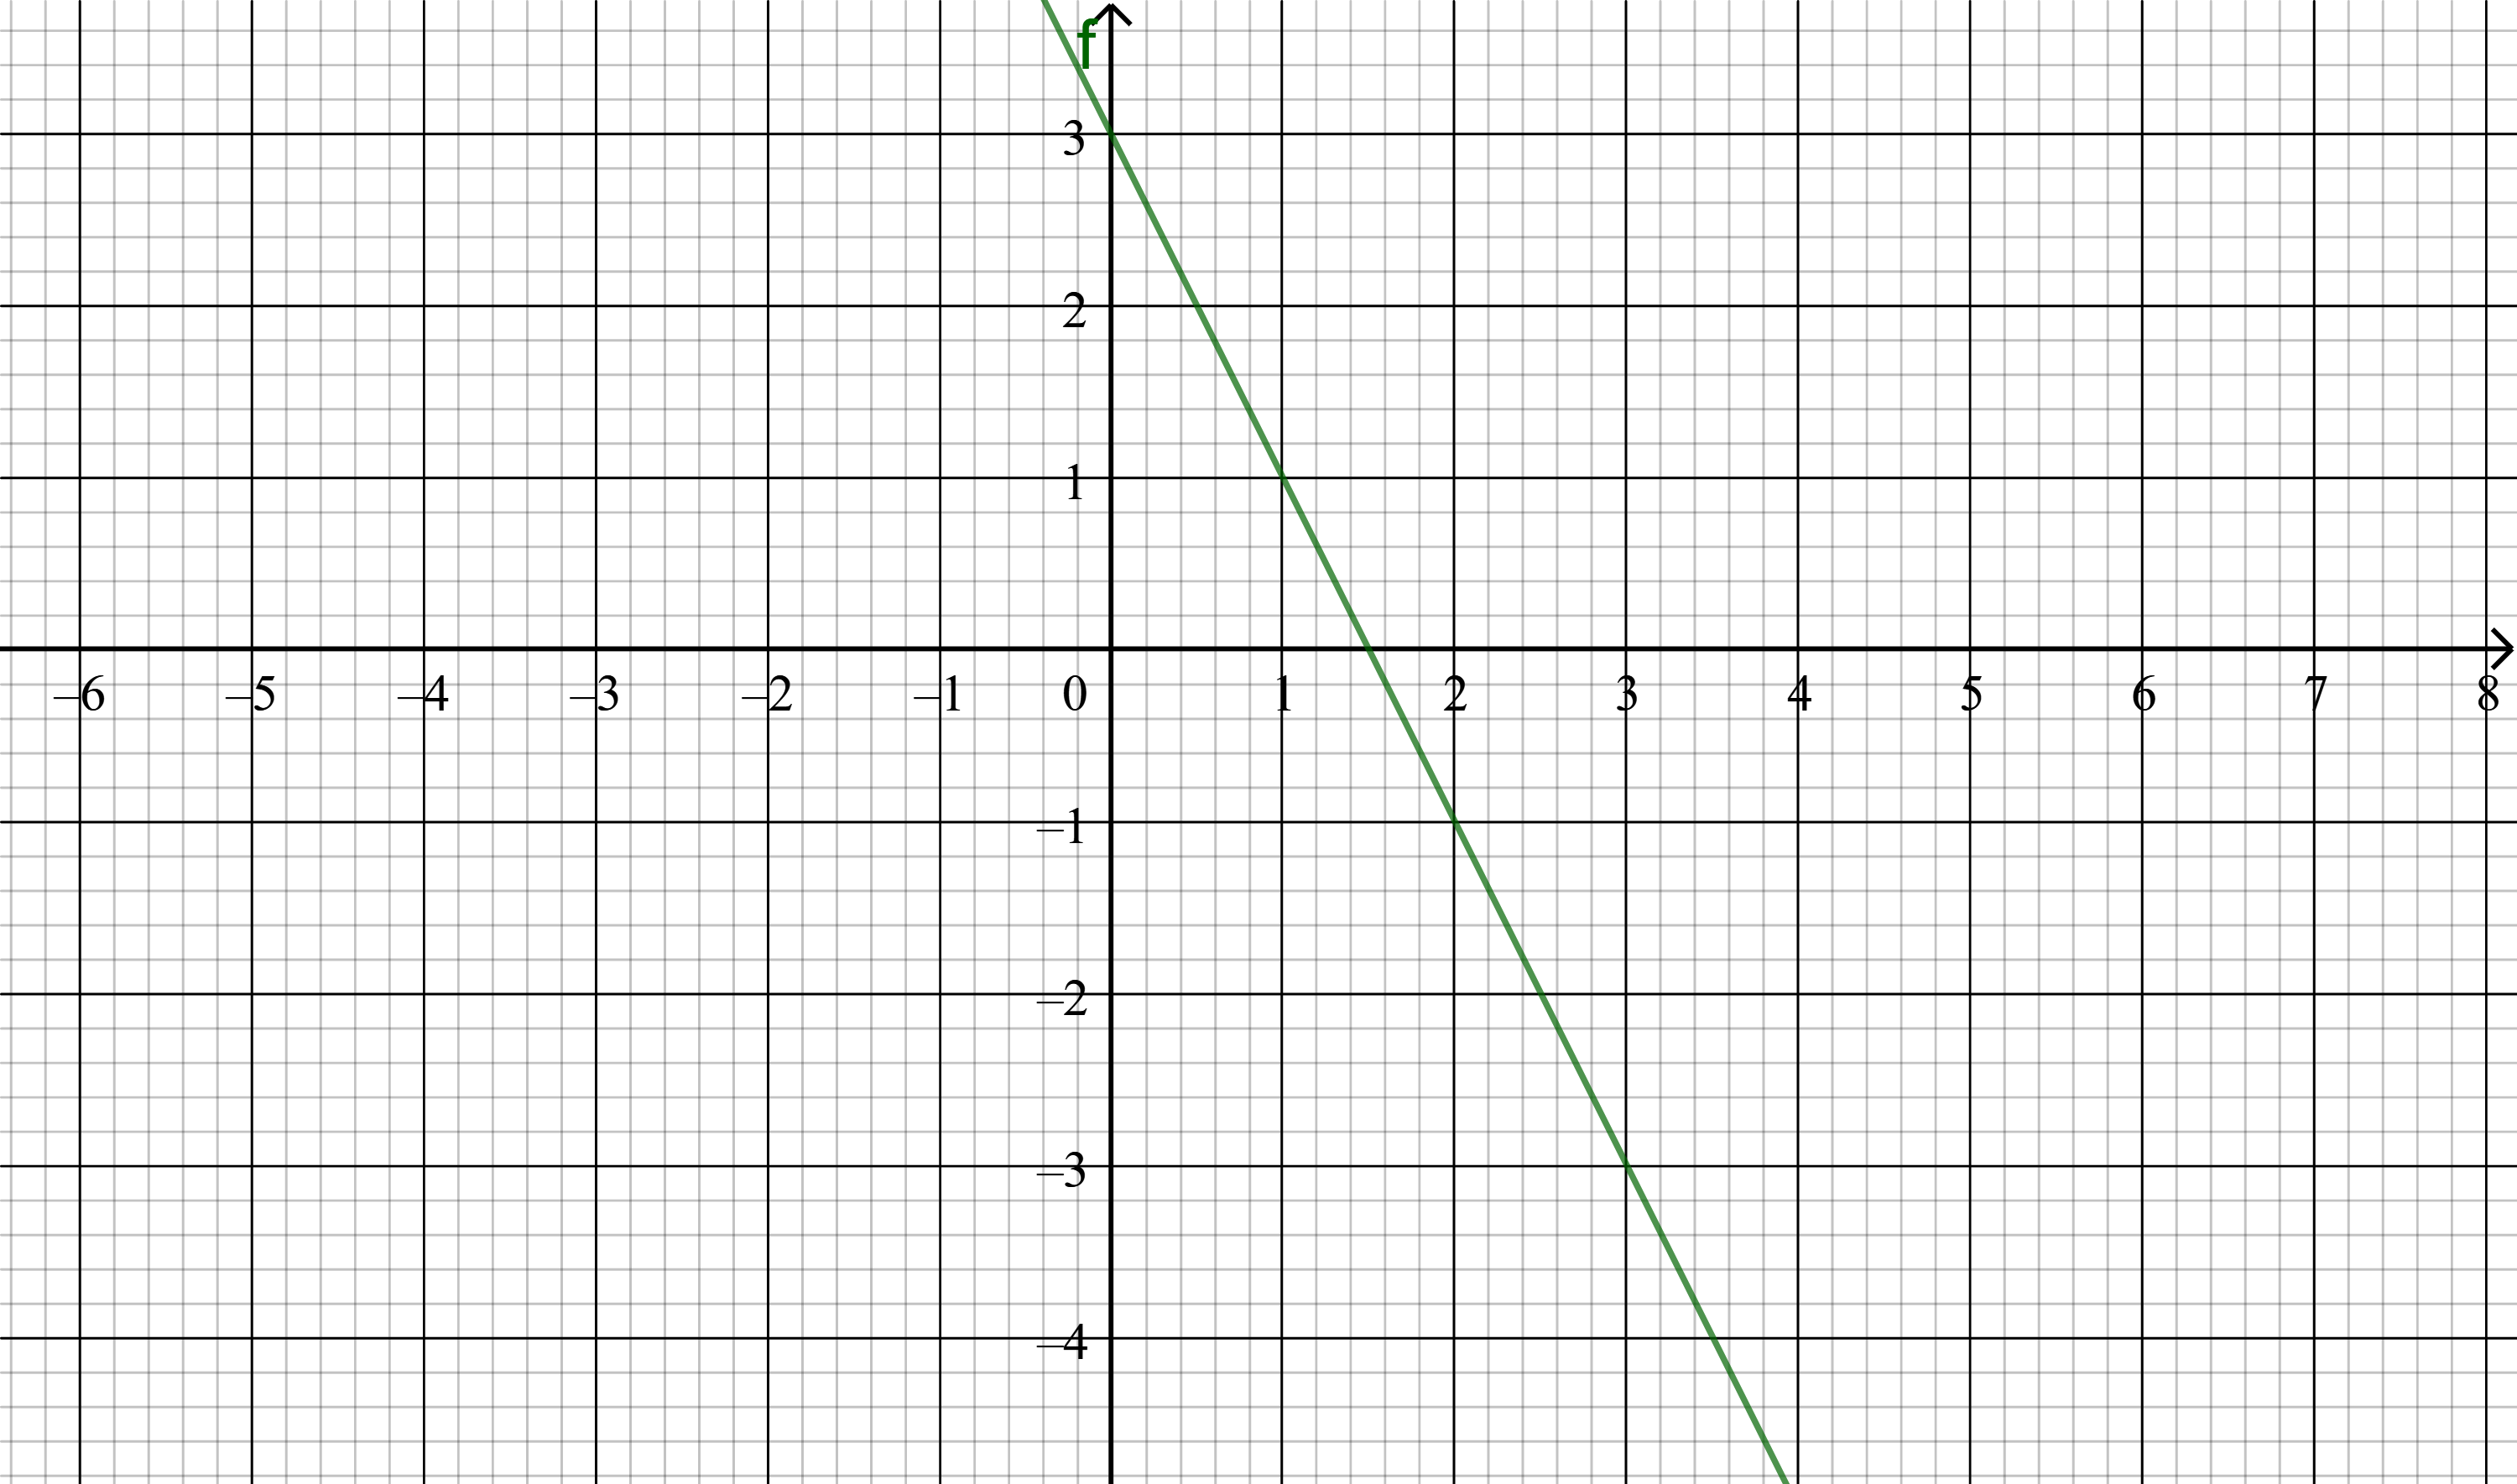
\includegraphics[width=0.5\textwidth]{pics/LinFunktion5}\\
 Bestimme die Funktionsgleichung von f. }
    \solution{ $f(x)=-2x+3$ }
    \end{Add}
    

        \begin{Add}{NeO}{basal1}{Begrifflichkeiten}{mittel}
        \question{ Formuliere sprachlich: \\
\begin{tabular}{rrr}  $x \leq 2$ & $x \geq 2$ & $x \neq 2$ \end{tabular} }
        \solution{ }
        \end{Add}
        \begin{Add}{NeO}{basal1}{Begrifflichkeiten}{mittel}
        \question{ Formuliere sprachlich: \\
\begin{tabular}{rrr}  $x \leq 2$ & $x \geq 2$ & $x \neq 2$ \end{tabular} }
        \solution{ \begin{tabular}{rrr} x ist höchstens 2 & x ist mindestens 2 & x ist ungleich 2 \end{tabular} }
        \end{Add}
        

\begin{Add}{NeO}{basal1}{Termumformungen}{mittel}
\question{ Sind die beiden Terme $a+((b \cdot c)-3)$ und -3+a+bc äquivalent? }
\solution{ }
\end{Add}
\begin{Add}{NeO}{basal1}{Termumformungen}{mittel}
\question{ Sind die beiden Terme $a+((b \cdot c)-3)$ und -3+a+bc äquivalent? }
\solution{ Ja }
\end{Add}

\begin{Add}{NeO}{basal1}{Grundoperationen}{leicht}
\question{ Runde 1.235 auf drei Werteziffern }
\solution{ }
\end{Add}
\begin{Add}{NeO}{basal1}{Grundoperationen}{leicht}
\question{ Runde 1.235 auf drei Werteziffern }
\solution{ 1.24 }
\end{Add}

\begin{Add}{NeO}{basal1}{Grundoperationen}{mittel}
\question{ Runde 12 auf eine Werteziffer }
\solution{ }
\end{Add}
\begin{Add}{NeO}{basal1}{Grundoperationen}{mittel}
\question{ Runde 12 auf eine Werteziffer }
\solution{ 10 }
\end{Add}

\end{document}
